%%%%%%%%%%%%%%%%%%%%%%%%%%%%%%%%%%%%%%%%%%%%%%%%%%%%%%%%%%%%%%%%%%% 
%                                                                 %
%                            ROOT FILE                            %
%                                                                 %
%%%%%%%%%%%%%%%%%%%%%%%%%%%%%%%%%%%%%%%%%%%%%%%%%%%%%%%%%%%%%%%%%%% 
%
%  Run LaTeX or pdfLaTeX on this file to produce your thesis.
%  To produce the abstract title page followed by the abstract,
%  see the file abstitle-phd.tex or abstitle-mas.tex.
%
%%%%%%%%%%%%%%%%%%%%%%%%%%%%%%%%%%%%%%%%%%%%%%%%%%%%%%%%%%%%%%%%%%%

\documentclass[chap,openright]{thesis}  %twoside,   12pt, 
% Use the first command below if you want captions over 1 line indented. A side
% effect of this is to remove the use of bold for captions (thesis default).
% To restore bold, also include the second line below.
%\usepackage[hang]{caption}      % to indent subsequent lines of captions
%\renewcommand{\captionfont}{\bfseries} % bold caption (needed with caption 
                                       % package to restore boldface.)
% \setstretch{1.5} 
% \renewcommand\chaptersize{\large}
% \renewcommand\sectionsize{\large}
% \renewcommand\subsectionsize{\normalsize}
% \renewcommand\subsubsectionsize{\normalsize}
% \renewcommand{\bibalign}{}

% \usepackage{subcaption}
%\captionsetup{compatibility=false}
% \usepackage{float}
% \usepackage{caption}
\usepackage[labelsep=period,justification=centering]{caption}
\renewcommand{\captionfont}{\bfseries}
\bibliographystyle{IEEEtran_rpi}
\usepackage{amsmath}
\usepackage{amsfonts}
\usepackage{amssymb}
\usepackage{amsthm}
\usepackage{mathtools}
\usepackage{commath}
\usepackage{rotating}
\usepackage[linesnumbered,ruled]{algorithm2e}
\SetKwInOut{Parameter}{parameter}
\usepackage[textsize=small,textwidth=1.75in]{todonotes}
% \usepackage{setspace}
\usepackage{xspace} % needed for \eg, \ie, \etc
% hyperref must be last
%When submitting your thesis, comment out hyperref
% -- courtesy of Dan Ibanez
\usepackage[hidelinks]{hyperref}

\renewcommand*{\UrlNoBreaks}{\do\(\do\[\do\{\do\<\do\:}%

%\usepackage{hyperref}
%\hypersetup{
%  colorlinks=true,
%  linkcolor=blue,
%  citecolor=blue,
%  urlcolor=blue
%}
\usepackage{multirow}
\newtheorem{definition}{Definition}[section]
\newtheorem{theorem}{Theorem}
\newtheorem{remark}{Remark}

\usepackage{cleveref}
\usepackage{booktabs}
\usepackage{siunitx}
\usepackage{caption}
\usepackage{longtable}
\captionsetup[longtable]{labelfont=bf,textfont=bf}
\usepackage{array}
\usepackage{lscape}


\usepackage{graphicx}
\usepackage{float}
%\usepackage{subcaption}    % clashes with \subfig package below
\usepackage[caption=false]{subfig}
\usepackage{url}

\newcommand{\etal}[0]{{\em et~al.\@}\xspace}
\newcommand{\eg}[0]{{e.g.\@}\xspace}
\newcommand{\ie}[0]{{i.e.\@}\xspace}
\newcommand{\viz}[0]{{viz.\@}\xspace}
\newcommand{\resp}[0]{{resp.\@}\xspace}
\DeclareMathOperator{\mydiag}{diag}
\newcommand{\comment}[1]{}
\newcommand{\mat}[1]{\ensuremath{\mathsf{#1}}}
\newcommand{\nsig}[0]{\ensuremath{n_{\mat{\Sigma}}}}


\usepackage{lipsum}

\newcommand\blfootnote[1]{%
  \begingroup
  \renewcommand\thefootnote{}\footnote{#1}%
  \addtocounter{footnote}{-1}%
  \endgroup
}


% \PassOptionsToPackage{usenames,dvipsnames}{xcolor}

% \usepackage{colortbl}
% \newcommand{\padd}[1]{{\leavevmode\color{blue}{#1}}}

% \usepackage{color, colortbl}
%\definecolor{blue}{rgb}{0,0.75,1}
%\definecolor{yellow}{rgb}{1,1,0}

% \includeonly{rpichap1}  % use \includeonly to process only
                         % the file(s) listed inside the braces        
% \begin{singlespace}
% \end{singlespace}

     
\begin{document}
%%%%%%%%%%%%%%%%%%%%%%%%%%%%%%%%%%%%%%%%%%%%%%%%%%%%%%%%%%%%%%%%%%% 
%                                                                 %
%                            TITLE PAGE                           %
%                            PhD Thesis                           %
%                                                                 %
%%%%%%%%%%%%%%%%%%%%%%%%%%%%%%%%%%%%%%%%%%%%%%%%%%%%%%%%%%%%%%%%%%% 
%  This file produces the title page, copyright page (if requested)
%  and the Table of Contents, List of Figures and List of Tables.
% 
%  To produce the abstract title page followed by the abstract,
%  see the template file, "abstitle-phd.tex"
%%%%%%%%%%%%%%%%%%%%%%%%%%%%%%%%%%%%%%%%%%%%%%%%%%%%%%%%%%%%%%%%%%%
    
% Supply information for use on title page:
%   
\thesistitle{\bf A Matrix-free Algorithm \\for reduced-space PDE-constrained Optimization}        
\author{Pengfei Meng}        
\degree{Doctor of Philosophy}        
\department{Aeronautical Engineering} % provide your area of study here; e.g.,
%  "Mechanical Engineering", "Nuclear Engineering", "Physics", etc.   
     
\signaturelines{4}     %max number of signature lines is 7        
\thadviser{Jason E. Hicken}
 %\cothadviser{Second Adviser} % If you have 2 thesis advisers
\memberone{Assad A. Oberai}        
\membertwo{Lucy T. Zhang}        
\memberthree{John E. Mitchell}
%\memberfour{Marcus Aurelius} % must change signaturelines to 5 if using this 5 members
%\memberfive{Marcus Junius Brutus} % must change signaturelines to 6 if using this 6 members
%\membersix{Nikola Tesla} % must change signaturelines to 7 if using this 7 members

\submitdate{April 2018}         %  \\(For Graduation January 2018)
\copyrightyear{2018}   % if omitted, current year is used.        

% Print titlepage and other prefatory material:
%    
\titlepage    
%\vfil
%\begin{flushleft}
%PhD life is nonlinear, most of the time it stays flat and boring, until it's not. 
%\end{flushleft}
%{\raggedleft Pengfei Meng \quad \par} 
%\vfil
\copyrightpage         % optional           
\tableofcontents        
\listoftables          % required if there are tables
\listoffigures         % required if there are figures


   
%%%%%%%%%%%%%%%%%%%%%%%%%%%%%%%%%%%%%%%%%%%%%%%%%%%%%%%%%%%%%%%%%%% 
%                                                                 %
%                         ACKNOWLEDGEMENT                         %
%                                                                 %
%%%%%%%%%%%%%%%%%%%%%%%%%%%%%%%%%%%%%%%%%%%%%%%%%%%%%%%%%%%%%%%%%%% 
 
\specialhead{ACKNOWLEDGMENT}
 
This dissertation is the essence of the not-so-short four and half years' work in the Optimal Design Lab of Professor Jason E. Hicken at Rensselaer Polytechnic Institute.  The PhD experience has taught me numerous valuable lessons in doing research,  given me sharper insights in numerical optimization field, and confidence in doing whatever is waiting ahead.  

I would like to thank my advisor, Professor Jason E. Hicken, without whom this thesis would not have been possible. I am grateful for the numerous discussions he patiently had with me whenever I run into problems. His broad knowledge and insights in numerical simulation and design field continues to motivate me.  Beyond being professional, he is an extremely nice person to work with, and it is my pleasure to have him as my advisor. 

I thank my doctoral committee members, Prof. Assad A. Oberai, Prof. Lucy T. Zhang, Prof. John E. Mitchell for the time they spend on my candidacy and thesis defense. Their valuable inputs greatly help improve the quality of my thesis work. 

Many thanks to my fellow lab mates in CII lab for providing a lively and humorous environment, Alp Dener, Anthony Ashley,  Jared Crean, Jianfeng Yan, Kinshuk Panda. In particular, thank Alp Dener, whose work in Kona laid the foundation for my thesis research, and who had very generously given me numerous valuable suggestions. 

I gratefully acknowledge Dr. Gaetan Kenway, Dr. Charles (Sandy) Mader in MDO design lab at University of Michigan for their help with the CFD solver ADflow. 

I am indebted to my mom for her constant support and love, despite the long distance and long time separation caused by my studying in the U.S.. My only sister, for the special bond we had through the rough days, and for your love and trust in me all the time. 

Yongjian Yang, thank you for being my life companion, and the meanings and purposes you instill to my life. I am grateful for having my baby daughter Emma. Everyday is a surprise with you. The lively energy you emits is my greatest source of happiness and inspiration.  

This thesis is jointly funded by NASA Learn project, Prof. Hicken's startup grant, and TA funding from the MANE department. Specially, thank OGE at RPI for supporting me with Childbirth Accommodation in fall 2017 after my baby was born, which enables me to spend more time with my baby and smoothly finish my PhD. 
   
%%%%%%%%%%%%%%%%%%%%%%%%%%%%%%%%%%%%%%%%%%%%%%%%%%%%%%%%%%%%%%%%%%% 
%                                                                 %
%                            ABSTRACT                             %
%                                                                 %
%%%%%%%%%%%%%%%%%%%%%%%%%%%%%%%%%%%%%%%%%%%%%%%%%%%%%%%%%%%%%%%%%%% 
 
\specialhead{ABSTRACT}
 In this thesis, a Reduced-Space Newton-Krylov method with Homotopy globalization technique is presented to solve PDE-constrained optimization problems.  
 
In the context of PDE-constrained optimization problems, 
%besides the design variables, the state variables also come into play. 
the objective and some of the constraint functions would depend on both the design and state variables. The  
total derivatives of the state-based objective and constraints necessitate an adjoint solve for each, which can be as expensive as the PDE solves. In the presence of many state-based constraints, it may not be practical to compute the constraint Jacobian explicitly. Besides, PDE-constrained problems can be very large, and 
%the dimension of PDE-constrained problems are usually very large, 
 storing the Jacobian matrices puts a heavy load on the computer memory.  A matrix-free Newton-Krylov optimization algorithm avoids these problems but presents additional challenges related to globalization, preconditioning, and inequality constraint handling abilities. 

To address these challenges, this thesis uses a globally convergent homotopy continuation approach to solve the first-order optimality conditions using reduced-space Newton-Krylov methods. It uses a predictor-corrector algorithm to trace the solution curve of the homotopy map that gathers the KKT condition and a homotopy regularization term. During the tracing process, the predictor and corrector linear systems are solved loosely by Krylov iterative methods. The matrix-vector products of the KKT matrix are approximated using second-order adjoints. This way, the computational cost of calculating the constraint Jacobians and memory cost of storing them are saved.  To cope with the poorly conditioned KKT system, matrix-free preconditioners based on Lanczos SVD approximation are proposed to accelerate the convergence of the Krylov iterative solvers.  

The proposed algorithm and preconditions are tested on a variety of problems. To verify its globalization ability, an inequality constrained sphere problem is first tested to check whether the new method can bypass local maximum points. Then a constructed high-dimensional quadratic indefinite problem with randomly generated non-convex pattern and random starting points is exercised; the statistical performance of 1000 cases are presented. The scaling performance of the algorithm and the effectiveness of the preconditioner is studied on a series of constructed quadratic problems with increasing dimensions, while the convergence results are compared with those of a popular matrix-based active-set optimization algorithm. The algorithm and preconditioners are also applied on a subset of CUTEr test problems to examine its accuracy and robustness. Finally, two PDE-constrained optimization problems are tested: the first one is a complex stress-constrained mass-minimization problem, which serves the case as many state-based constraints; the second one is an aerodynamic shape of the NASA Common Research Model wing based on Euler equations. In both cases, the results using the algorithm and preconditioners from this work are compared with those using state-of-the-art matrix-based optimization algorithm SNOPT. 

%%%%%%%%%%%%%%%%%%%%%%% 
  
%%%%%%%%%%%%%%%%%%%%%%%%%%%%%%%%%%%%%%%%%%%%%%%%%%%%%%%%%%%%%%%%%%% 
%                                                                 %
%                            CHAPTER ONE                          %
%                                                                 %
%%%%%%%%%%%%%%%%%%%%%%%%%%%%%%%%%%%%%%%%%%%%%%%%%%%%%%%%%%%%%%%%%%% 
 
\chapter{INTRODUCTION}
 
\section{Motivation}
At the turn of 2017/2018,  global warming has been unequivocally proven by scientific evidence~\cite{nasa_warm}. 
The surface temperature of Earth has risen by 2.0 degrees Fahrenheit since the late 19th century.  The ice sheets, glaciers and Arctic sea ice are retreating almost everywhere on Earth, at an accelerating speed. Extreme weather like tornados, heatwaves, wildfires and droughts are increasing in frequency and intensity. There is no doubt that human activities, especially manmade emissions carbon dioxide (CO2) and other exhausts like nitrogen oxides, carbon monoxide, and sulphur oxides are the major causes. 

Air transport is responsible for about $2\%$ of the manmade carbon dioxide (CO2) emissions~\cite{aviation_warm}. But because of the altitude at which the CO2 is released, together with the fact that other emissions like NOx and water vapor have a larger impact on the climate at higher altitudes, researchers suggest that the share of the aviation CO2 emissions should be multiplied by 1.9 times to incorporate the impact of altitude and other exhausts.   

With the number of airplane passengers increasing at an average of $5\%$ each year, perhaps more in developing markets, the impact of aviation on the environment will only increase. It is estimated that approximately 27,000 new passenger aircrafts will be demanded between now and 2030.  The total contribution of aviation to human emissions in CO2 and other effects will rise to $5\%$ and in a worst-case to $15\%$. 

Advisory Council for Aeronautics Research in Europe (ACARE) is enforcing strict emission targets, to reduce CO2 emissions per passenger kilometer by $75\%$, NOx by $90\%$ and perceived noise by $65\%$ by 2050 relative to the year 2000~\cite{SKINNER2018933, euro_commi}. Reducing the impact on the environment is becoming the driving factor for future aircraft design~\cite{green_2006}. To do that, the aviation industry needs to continue working on reducing gas emissions by using lightweight and smart materials, and optimizing current aircraft configurations. 

%technology, like exploring innovative aircraft shapes, improving current aircraft efficiency by minimizing drag for aerodynamic shape optimization, or minimizing mass for structural optimization, and upgrading operations to reduce noise and delays. 

\section{The Role of Numerical Optimization}
The ultimate goal of engineering is to make better decision-making models through optimization. Numerical optimization plays a key role in almost every aspect of engineering design.  

The aircraft design is a complicated system that involves aerodynamics, structures, propulsion, stability, mission and whole performance. The past two decades has seen growing interest in using optimization to explore unconventional aircraft configurations like the blended-wing body (BWB), the Box Wing, and the UCAV (Unmanned Combat Air Vehicle). During the conceptual 
aircraft design stage, numerical optimization can reveal valuable insights about the design trade-offs and help engineers make detailed and informed decisions.  
     
The first aerodynamic optimization was done in \cite{hicks:1974} by using finite-difference approximations to calculate the gradients. The cost of computing the gradients using finite-difference methods increases drastically as the design dimension increases. The adjoint methods have greatly propelled the advancement of research in aerodynamic shape optimization field. Adjoint methods address the dimensionality issue of finite-differences with a cost independent of the number of design variables. \cite{pironneau:1974} developed the adjoint method for Stokes equations and the incompressible Euler equations, and used the adjoints to optimize airfoil profiles. \cite{reuther:1996} used an adjoint algorithm based on Euler to optimize a complete aircraft configurations.  \cite{jameson:1988} derived the adjoint equations for inviscid compressible Navier-Stokes equations, making it possible to do transonic aerodynamic optimizations.  The discrete adjoint method is more preferred in aerospace optimization as the sensitivities are exact to the discretized objective function~\cite{frank:1992}. \cite{Mader06adjoint:an} derived a discrete adjoint method for Euler equations using automatic differentiation. \cite{Lyu2013b} extended the previous adjoint implementation to 
Reynolds-averaged Navier-Stokes (RANS) equations and effectively applied it to high-fidelity optimization. \cite{hicken:aiaa2010} developed similar methods for non-planar wings high-fidelity aerodynamic optimization. 


%The ever-growing capacity of computers are empowering numerical analysts to do simulations on ever-larger physics systems governed by Partial-Differential-Equations(PDEs). Accordingly, PDE-constrained optimization problems pose greater challenges as the optimization systems are larger and more complicated, especially when many state-based constraints are present. Current matrix-based optimization algorithms are defied for such problems due to memory requirements and computing cost. 


\section{PDE-constrained Optimization Framework}
This thesis is interested in solving engineering design optimization problems that are governed by Partial-Differential-Equations (PDEs). Such PDE-constrained optimization problems arise in many engineering applications including aerodynamic shape optimization \cite{lambe:2014,lyu2014aerodynamic, Zhang567303}, structural optimization \cite{DBLP:DeckelnickHJ17, lambe:2014, kennedy14}, and thermodynamic optimization \cite{chen1999finite,bejan2000thermodynamic,bejan2012thermodynamic}.  %


\begin{figure}[H]
\centering
\subfloat[Aero-Structure Optimization~\cite{as_opt}]{
  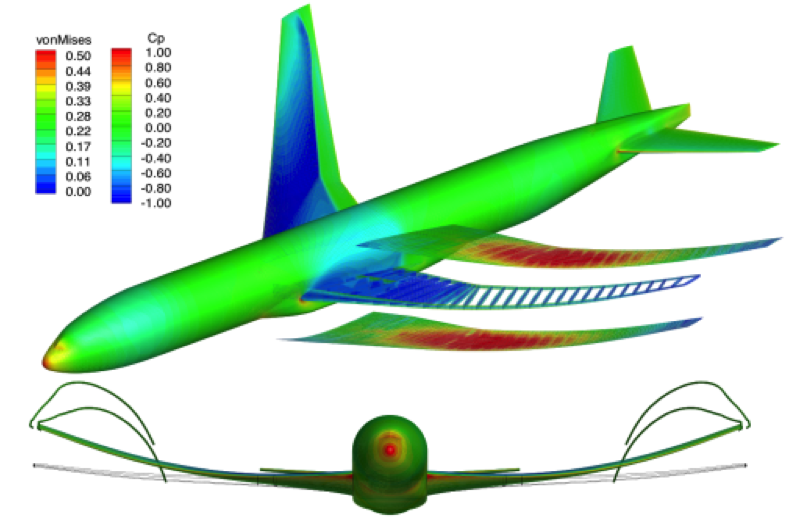
\includegraphics[clip,width=0.5\columnwidth]{./figs/chap1_intro/1_as.png}\label{fig:A}  %
}
\subfloat[Topology Optimization~\cite{topo_opt}]{ %
  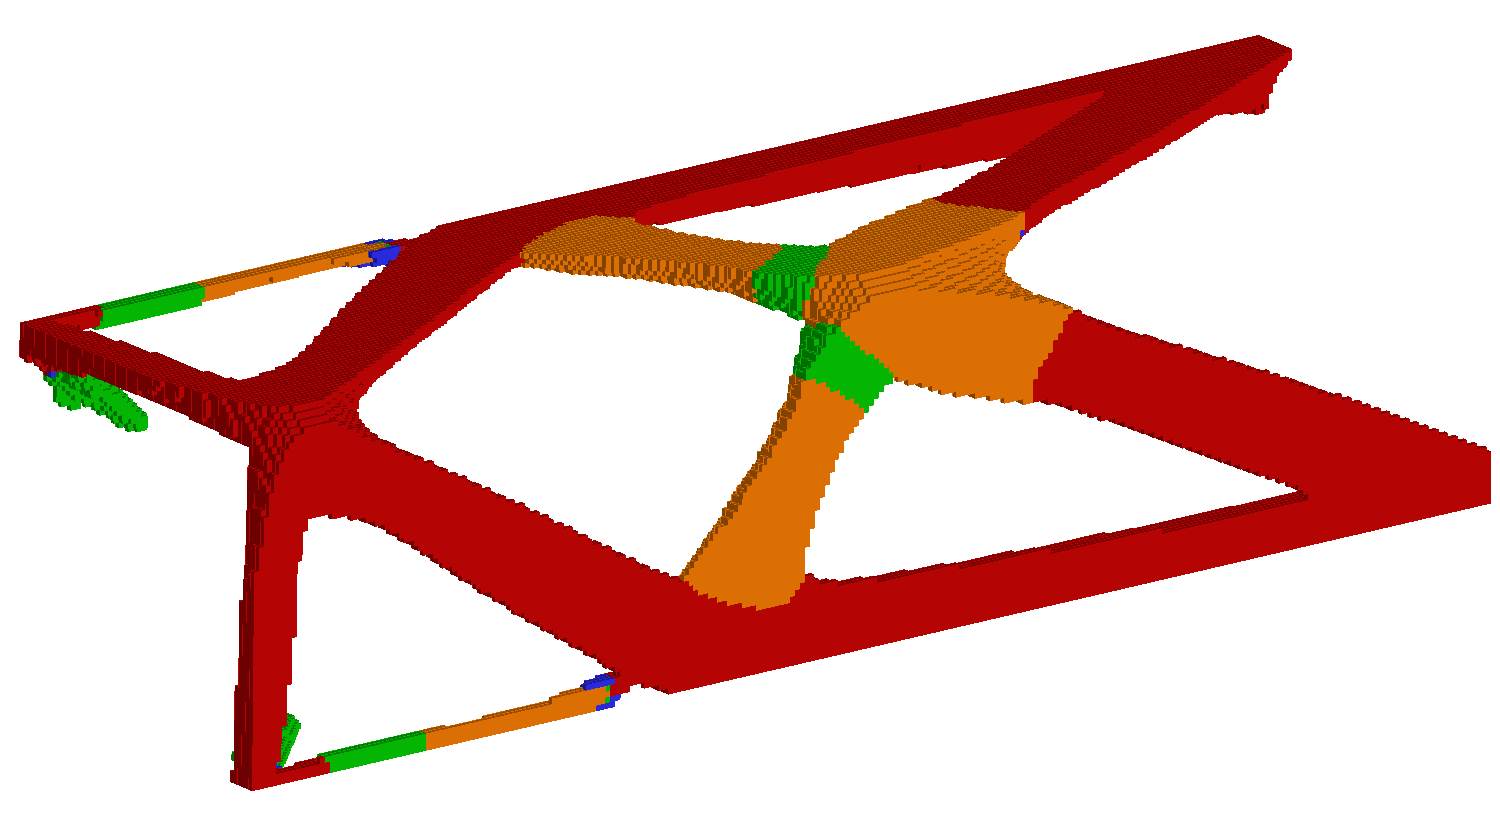
\includegraphics[clip,width=0.5\columnwidth]{./figs/chap1_intro/1_topo.png}\label{fig:B}
}
\caption{Large-Scale PDE-constrained Optimization}
\label{fig:1_mot}
\end{figure}

In such applications, an optimization library is coupled with a PDE solver. The simulation problem solves the PDEs for state variables, e.g. the pressure distribution along the surface mesh node points on the wing in Figure~\ref{fig:A}, and the displacement distribution among the solid mesh node points in Figure~\ref{fig:B}, at certain design variables. The performance of the physics system is evaluated in the form of objective function bounded by certain constraints, while the objective and the constraints depend on both the state variables and the design variables. The optimizer will choose a design point, inquire the PDE solver for state variables, and compute the functional values and the gradients of the objective and constraints at that point. The optimizer will process all the information and yield a better design point using mathematical algorithms. The process is repeated until certain criteria is met for optimality.  

The optimization framework is simple, and has been used successfully in many application fields. The difficulty in PDE-constrained optimization is that the PDE solution (or state equation), which itself is a complicated topic to which intensive effort has been devoted, is a sub-problem of the optimization problem. During the optimization process, the optimizer will query the PDE solver many times for the state variables and gradients at different design points; in addition to that, the optimizer needs to compute and store the gradients of the constraints and objective in order to determine the next design point. However, in large-scale engineering, the PDE solve and gradient evaluation can be very expensive even with the advancement in modern computer power. Moreover, storage of the necessary matrices can impose a heavy burden on computational resources.    

General-purpose optimization algorithms are unsuitable for large-scale PDE-constrained optimization problems because their matrix-based approaches require the computation and storage of the total constraint Jacobians, which in turn would result in poor scalability performance with ever-increasing size of problems. In addition, the commonly used limited-memory quasi-Newton methods in general-purpose algorithms usually bring linear asymptotic convergence rates, which are not ideal for large-scale optimization problems. 

This thesis intends to address these challenges by proposing a scalable optimization algorithm especially intended for large-scale PDE-constrained design problems. 

\section{Optimization Algorithms}
Many optimization packages are available for applications of different types. Considering the expensive cost of PDE solutions in PDE-constrained optimization problems, it is crucial to choose an efficient optimization algorithm that uses fewer function evaluations. In addition, the optimization algorithm must be able to handle nonlinear objectives and constraints. Gradient-free optimization algorithms like the genetic algorithm are not suitable here because they demand large number of function calls, despite the fact that they can locate global minimums. Gradient-based algorithms are used extensively in PDE constrained optimizations as they can handle hundreds of design variables by using the adjoint method to compute the gradients, with fewer function evaluations.  \cite{2015lyu_crm} and \cite{kenway:2014} use SNOPT (Sparse Nonlinear OPTimizer) \cite{gill:2002} through the Python interface pyOpt~\cite{Perez:2011:A} for the investigations of the aerodynamic and aerostructural optimization on the Common Research Model based on RANS, using analytically-derived adjoint gradients. Because there are only three aerodynamic objective and constraints, drag, lift, and pitch moment coefficients, they use the adjoint methods to assemble the total gradients to SNOPT. Other general purpose optimization algorithms, IPOPT~\cite{Lyu2014f}, Knitro~\cite{Rumpfkeil2009OptimizationbasedMA}, and a sequential quadratic programming method~\cite{Ning09multidisciplinaryconsiderations, can also work for aerodynamic design problems, }. But they all compute the total gradients by using the adjoint methods and feed that to the optimization algorithm. 

For PDE-constrained optimization problems, when there are many state-based constraints, assembling the total constraint Jacobian is very expensive as it demands an adjoint solve for each state-based constraint. Additionally, general optimization algorithms store the constraint Jacobians at each design point, which puts a heavy memory load on the computer. Therefore, most general optimization algorithms possess poor scaling qualities.  

For these reasons, optimization researchers in different PDE fields have been developing in-house algorithms for their own use. For detailed formulations, see chapter~\ref{sec:pde_mot}. Newton-based full-space methods possess good scaling, but are complicated to implement as they require intrusion to the PDE solver. Currently, no general purpose optimization libraries exist for full-space methods.  In addition, other numerical difficulties exist for full-space methods as pointed out in chapter~\ref{sec:pde_mot}. In comparison, reduced-space methods possess modularity that can make good use of prevalent PDE solvers. \cite{rumpfkeil:2010b} uses a reduced-space Newton algorithm in Knitro to perform steady and unsteady aerodynamic shape optimization, with less computational cost compared with a quasi-Newton method; but the reduced Hessian is computed explicitly. In this work, we present a general reduced-space Newton-Krylov optimization algorithm, which is part of the matrix-free optimization package Kona~\cite{dener:scitech2016}, for PDE-constrained optimization problems. It possesses good algorithmic scaling property as it approximates Hessian vector products through second adjoint solves. In addition, a Lanczos based preconditioner 
is presented to accelerate the convergence of the iterative linear solvers.  

%Conventionally, solving general constrained optimization problems without PDE constraints involves forming the Lagrangian, and finding the minimization point of the Lagrangian, which is equivalent to solving the first-order optimality conditions or the KKT conditions. Prevalent sequential quadratic programming methods or newton-type methods for solving a system of equations would further break it down to solving a series of systems of linearized equations, also called the Karush-Kuhn-Tucker (KKT) system. The KKT matrix contains the Hessian of the Lagrangian, which is often approximated using quasi-Newton method, and the total constraint Jacobians, which is straightforward to compute using automatic differentiation or complex step methods. Conventional matrix-based optimization algorithms would use direct factorization methods to solve the KKT system.    


\section{Preconditioners for Optimization}
Using Krylov methods to solve the linear systems saves the effort of computing and storing the constraint Jacobian and Lagrangian Hessian, but the convergence rate of Krylov solvers depends on the distribution of eigenvalues of the system matrix. If the eigenvalues are clustered in a small radius, the convergence rate is better. Poor convergence happens when the ratio of the largest to the smallest absolute eigenvalue is large, ($10^5$ to $10^9$). 

In the context of the PDE-constrained optimization problem, there are two sources of ill-condition. The first one resides in PDE solvers. When the discretization is refined, some of the eigenvalues of the PDE system matrix could go towards zero, or in other words the PDE problem is ill-posed. The second source of ill-condition often arises from optimization algorithms themselves. For example in the interior-point method family, the slack variables are used to measure the activeness of the inequality constraints. When some of the inequality constraints get close to the boundary, the corresponding slack variables would approach zero, and some entries on the diagonal of the KKT matrix will go unbounded. The second type of ill-condition is the target in this thesis, as the first type is usually covered as part of the PDE solver.     

In presence of ill-conditioning, a nonsingular matrix, the preconditioner, could do similarity transformation to the linear system, resulting in a better conditioned system with the same solutions.   

Several popular preconditioners exist for general optimization problems without PDE constraints, like incomplete factorizations~\cite{saad:2003}, which involve direct operations to the entries of the matrix,
or the null space approach, which involves computing and working with the null space of constraint Jacobians to find the step updates. Those preconditioners would not work well for interior-point methods type optimization problems, as the diagonal entries could approach zero or infinity for inequality constraints. Specially, for matrix-free PDE constrained optimization problems, the Hessian or constraint Jacobian do not exist in explicit form, so it is not possible to use direct methods.  

Inspired by domain-decomposed Schur preconditioners used in PDE solvers~\cite{keyes_domain} ,  where approximate subdomain solutions of the mesh field are used as preconditioners for the iterative solver of the PDE, \cite{DBLP:journals/siamsc/BirosG05} uses approximate state and adjoint solutions in the Schur of the KKT system as the preconditioner for the Krylov solver in each Newton step for the optimization problem. \cite{pc_kkt_control} presented a similar KKT matrix preconditioner for  optimization in distributed control problems using an interior-point method; it also used the block structure of the KKT matrix to decompose it, then used existing preconditioners for the PDE solvers to approximately solve the preconditioning system. However, the preconditioner is not ideal as the preconditioned system has both positive and negative eigenvalues. In addition, \cite{doi:10.1137/15M104075X} constructed a preconditioner for the full-space Lagrange-Newton method for multi-field problems. The preconditioner removes the field variables that are causing nonlinearity of the system, resulting in a well-balanced Newton system. The preconditioner proposed in this thesis is similar to  that proposed in \cite{pc_kkt_control}. 

%The kernel of reduced-space Newton-Krylov methods for PDE-constrained optimization solves a series of linear systems, which are saddle point systems, but much smaller than the saddle-point system raised in full-space methods.  Because the solution to the optimization problem \eqref{eq:opt00x} is a saddle point for the Lagrangian \eqref{eq:lag} in that the optimal design point minimizes the Lagrangian, while the optimal multipliers maximizes the Lagrangian ~\cite{benzi2005numerical}.  

\section{Thesis Objectives and Outline}

%The objective of this thesis is to develop an efficient inexact-Newton algorithm that is
%suitable for reduced-space PDE-constrained optimization problems of the
%form~\eqref{eq:gen1}.  This goal faces two significant challenges, which
%we seek to address in this work.
This thesis aims to overcome the challenges listed below, and in doing so represents 
two separate objectives. 

\begin{description}
\item[Nonconvexity:] The system $F(q) =0$ does not distinguish between different
  types of stationary points, so a basic Newton's method may converge to local
  maximizers or saddle points.  Conventional optimization algorithms often
  project onto the null-space of the (active) constraint Jacobian to detect
  directions of negative curvature and avoid undesirable stationary points, but
  the null-space is not explicitly available for matrix-free inexact-Newton
  methods.
\item[Preconditioning:] The number of iterations necessary to satisfy the
  inexact Newton condition \eqref{eq:inexact_Newton} using, for example, a
  Krylov method is closely related to the condition number of the system.
  Unfortunately, it is well known that the primal-dual, or KKT, matrix $\nabla_q
  F$ is indefinite and highly ill-conditioned.  A preconditioner is needed that
  is inexpensive to form, factor, and store.  A general-purpose, inexpensive
  preconditioner is especially difficult to find in the reduced-space context,
  since approximations to $\nabla_q F$ are not readily available as they are in
  the full-space.
\end{description}

The approach to addressing globalization is to introduce a homotopy map that
implicitly defines a solution curve that connects the solution to an easy
problem to the solution of the desired problem.  We then use a
predictor-corrector algorithm to follow the curve from the easy to the desired
solution.  A related globalization is used in \cite{Perez2009homotopy} in the
context of a trust-region managed sequential approximate optimization.  To
address the conditioning of the KKT matrix, we propose a low-rank approximation
of the Schur complement that is constructed by applying a few iterations of the
Lanczos method with approximate adjoints.

The following contents are organized as follows: 
\begin{itemize}
\item Chapter 2 lays out the mathematical foundations for the whole work. The first-order optimality conditions 
for the reduced-space method that we are aiming to solve, the inexact-Newton methods that we use to solve it, 
together with Krylov iterative method are all briefly explained. 

\item Chapter 3 reviews homotopy-based globalization and the homotopy map adopted in this work. Then it describes the predictor-corrector path-following algorithm that traces the homotopy zero curve using Newton-Krylov method. To verify the proposed globalized algorithm, a Sphere problem with a linear objective and quadratic inequality constraints is tested. Then a constructed indefinite problem is used to examine the algorithm's ability to bypass local maximum points. 

\item Chapter 4 is focused on describing the proposed matrix-free preconditioner, firstly for solving inequality constrained problems, then for solving problems with both equality and inequality constraints. A constructed quadratic problem with linear inequality constraints is used to investigate the effectiveness of the inequality preconditioner and the scalability performance of the algorithm. 

\item Chapter 5 begins with briefly introducing the optimization environment Kona, a state-of-the-art optimization algorithm SNOPT against which the performance of the new method is compared, and the parameter settings for the new method.  Then it briefly introduces the CUTEr problem format, its classification and the Kona-CUTEr interface. Lastly the proposed optimization algorithm and preconditioners are tested on a subset of the CUTEr problems. 
  
\item Chapter 6 applies the algorithm and the preconditioners on two engineering design problems: firstly on a mass minimization stress-constrained structural problem, where the results and the convergence history of the algorithm are compared with that of SNOPT; secondly on an aerodynamic shape optimization problem. 

\item Chapter 7 provides conclusions and some suggestions for future works. 
\end{itemize}


% a popular large-scale matrix-based active -set augmented-Lagrangian optimization method SNOPT.  

%\begin{equation}\label{eq:saddle}
%\mathcal{A} = \begin{bmatrix}
%A & B \\
%C & D
%\end{bmatrix}
%\end{equation}
%One type of Schur complement can be obtained by performing the following LDU decomposition 
%\begin{equation}\label{eq:saddle:ldu}
%\mathcal{A} = \begin{bmatrix}
%A & B \\
%C & D
%\end{bmatrix} = 
%\begin{bmatrix}
%I_p & BD^{-1} \\
%0 & I_q
%\end{bmatrix}
%\begin{bmatrix}
%A-BD^{-1}C  & 0 \\
%0  & D 
%\end{bmatrix}
%\begin{bmatrix}
%I_p  & 0 \\
%D^{-1}C  & I_q 
%\end{bmatrix}
%\end{equation}

% which is indefinite, poor spectral properties (ill-conditioned) 
% Direct solvers, however, are still the preferred method in optimization and other areas. Furthermore, direct methods are often used in the solution of subproblems, for example as part of a preconditioner solve.
%The preconditioners developed here are tailored for PDE-constrained optimization problem. 
% matrix-vector products with A can be performed efficiently
% approximate its action on a vector with (nearly) linear complexity,
% the convergence of the iterates to the optimal solution of problem
% gain efficient, save on storage
%words from the paper ~\cite{benzi2005numerical} Benzi block preconditioners, 
% As the iterates approaches the solution,  the entries in A tend to zero, or infinity, KKT matrix ill-conditioned
% the norm of the inverse Schur complement goes to infinity

% Schur complement reduction 
% null space methods, the null space of the constraint Jacobian, the column of Z span the null space of constraint Jacobian
% popular in optimization, projection of the problem onto the constraint set; 

 
%%% Local Variables: 
%%% mode: latex
%%% TeX-master: t
%%% End: 

%The formula \eqref{eq:kkt0} takes the same form as the classical interior point method in Chapter 19 in Nocedal's book \cite{Nocedal2006NO}, which will be reviewed below. 

%\section{Review on Interior Point Method  }
%The difficulty in extending the Newton Krylov methods to handle inequality constraints, to solve \eqref{eq:opt00x} lies in the nonlinear complementarity condition: for each inequality constraint, either the slack or Lagrangian multiplier is strictly zero if we assume strict complementarity is satisfied at the solution. The slack has to be non-negative to guarantee feasibility of the inequality constraints, and the multipliers has to be non-positive in respect to the property of a local minimization point following the formula convention. For inequality constraints that are active at the solution, slack variable is zero and the multiplier is negative, while for inactive inequality constraints, slack variable is positive and the multiplier is negative. Therefore, the complementarity condition, in combined with the sign requirement on slack and multipliers, contains information on optimal active set of the inequality constraints at the solution.   
%
%Currently there are two most powerful algorithms for general nonlinear constrained problems: active-set SQP methods and interior point methods \cite{Nocedal2006NO}. Determining the inequality constraint sets that are active at the solution is the main challenge facing active-set methods. Especially when the number of inequality constraints is large, the method may need many iterations to locate the active-set of inequality constraints. While for interior point methods, there are two varieties based on globalization strategies: Newton-Lagrangian line-search and trust-region SQP on the barrier problems. The former is more for illustration purpose, and the latter is actually implemented in practical optimization software libraries IPOPT \cite{W�chter2006}, and KNITRO \cite{Byrd:1999:IPA:588897.589167}. 
%
%The trust-region SQP method builds a quadratic model on the barrier formulation, employs direct linear algebra, uses explicit constraint Jacobians to first compute the multipliers that deliver minimum linearized constraint violations, then compute the design and slack update steps that minimize the quadratic model. In both subproblems, a trust region bound is imposed on the design and slack components, with the slack variable scaled properly to prevent it away from the nonnegative bound. A proper merit function mimic the quadratic objective function is used to estimate the quality of the steps and control the trust-region radius for next iteration. 
%
%To handle nonlinearities and nonconvexities, regularization terms can be added to the Hessian block and the equality constraint Jacobian on the diagonal of the KKT matrix. The proper amount of regularization is computed at each iteration by trial and error such that the inertia of the regularized KKT matrix is $(n+m, l+m, 0)$, under which condition the total Hessian block of design and slack will be positive definite on the null space of the combined constraint matrix, therefore the resulted Newton step will be a guaranteed descent direction for a large class of merit functions. 
%
%Using the proper barrier parameter $\mu$ updating strategy is crucial to the performance of interior point methods: A slowly decreasing $\mu$ will result in large number of outer iterations, making the algorithm less efficient. While a quickly decreasing $\mu$ may make some slack or inequality multipliers approach zero prematurely, hurting the convergence. Some simple implementations of interior point methods use a constant fraction updating scheme, while some chooses the fraction value based on the recent iterations' progress towards the solution. Making the fraction value close to zero near the solution can yield a superlinear convergence rate. More robust strategies update $\mu$ based on the progress of the current complementarity products. Predictor strategy first calculates a predictor direction by setting $\mu=0$, then calculates the tentative complementarity product along this direction using the step size from fraction to boundary rule. The updating fraction value is based on the ratio of this tentative and current complementarity product. 
%
%
%The former Newton-Lagrangian line-search method solves a perturbed KKT system at each homotopy parameter, also called the barrier parameter $\mu$:
%
%\begin{equation}\label{eq:kkt1}
%\begin{aligned}
%\nabla f(x) + \lambda_h^T \nabla h(x) + \lambda_g^T \nabla g(x) &= 0 \\
%-\mathcal{S} \Lambda_g - \mu e &= 0\\
%h(x) &= 0 \\
%g(x) - s &= 0 \\
%s \geq 0, \quad &\lambda_g \leq 0 \\
%\end{aligned}
%\end{equation}
%The barrier parameter $\mu$, is a sequence of strictly positive numbers and converges to zero. The perturbed KKT system \ref{eq:kkt1} is solved for each $\mu$, and the solution trajectory converges to the KKT point of the original problem in the limit.  
%
%Newton's method is used to solve \ref{eq:kkt1} for each $\mu$, where each Newton step is as follows:
%\begin{equation}
%\begin{bmatrix} \mathcal{W} & 0 & \mathcal{A}_{h}^T & \mathcal{A}_{g}^T \\
%    0 & -\Lambda_g & 0 & -\mathcal{S} \\
%    \mathcal{A}_{h} & 0 & 0 & 0 \\
%    \mathcal{A}_{g} & -\mathcal{I} & 0 & 0 
%    \end{bmatrix}
%    \begin{bmatrix} p_x \\ p_s \\ p_h \\ p_g \end{bmatrix}
%    = -\begin{bmatrix} \nabla_x \mathcal{L} \\ -\mathcal{S} \Lambda_g - \mu e  \\ h(x) \\ g(x) - s \end{bmatrix}
%\end{equation}
%After the Newton step direction is computed, fraction to the boundary rule is applied to determine the maximum allowable step size to keep the slack and inequality multipliers away from the 0 bound. Then a backtracking line search is performed to find the step length that delivers sufficient decrease in the merit function or accepted by the filter. The barrier parameter is then updated for the next iteration. 
%
%There are potential drawbacks when using interior point methods for PDE-constrained optimization. For instance, to ensure progress towards global minimum, either trust-region or line-search globalization techniques have to be implemented. The former judges the quality of a computed step by calculating the merit function value and adjust the trust-region radius accordingly, while the latter computes the step-length along a step direction that satisfies the Wolfe condition. In either case, extra computation is needed. Dealing with nonconvex Hessian of the Lagrangian in the null space of the constraint Jacobian is also a non-trivial task; possible solutions include adding a proper regularization term to enforce a positive definite Hessian, see \cite{hicken:flecs2014} and Algorithm B.1 \cite{Nocedal2006NO}. Moreover, the saddle-point matrix raised in optimization is indefinite and ill-conditioned, making it difficult for iterative Krylov methods to converge. 


  
%%%%%%%%%%%%%%%%%%%%%%%%%%%%%%%%%%%%%%%%%%%%%%%%%%%%%%%%%%%%%%%%%%% 
%                                                                 %
%                            CHAPTER TWO                         %
%                                                                 %
%%%%%%%%%%%%%%%%%%%%%%%%%%%%%%%%%%%%%%%%%%%%%%%%%%%%%%%%%%%%%%%%%%% 
 
\chapter{HOMOTOPY-BASED GLOBALIZATION}\label{chap:homotopy}

\section{Homotopy-based Globalization}\label{sec:homotopy}
 \footnote{Portions of this chapter are extracted from the manuscript: P. Meng, A. Dener and J. E. Hicken, 
 Matrix-free Algorithm for Reduced-Space PDE-governed Optimization with Inequality Constraints.}
Homotopy methods are robust, numerically stable, and globally convergent methods
for solving nonlinear algebraic equations; see, for example,
\cite{allgower_georg_1993} and \cite{Watson_1989}.  The interest of this thesis in these
methods began as a means of globalizing difficult computational aerodynamics
problems~\cite{hicken:cfd2009, hicken:cfd2011b, Brown_2016}, but globally
convergent probability-one homotopy methods have also been successfully applied
to solve engineering optimization problems~\cite{WATSON1989289}.  Watson~\cite{Watson_2001} reviewed
and developed the general convergence theory of probability-one homotopies for nonlinear optimization
problems, including unconstrained, bound-constrained, linear and nonlinear
inequality constrained convex cases.  He also discussed the extension of the
theory to nonconvex problems, although the convergence theory for equality
constraints remains an open problem.  More recently, Huang
\etal~\cite{huang_2012pc} transformed a general nonlinear optimization with
equality and inequality into an inequality-only problem, and used a
predictor-corrector method to track the homotopy interior-point map using the
conjugate gradient method. While their method achieves global linear convergence
under the normal cone condition, it is limited to convex objectives and
constraint functions.

\subsection{Example}

Conceptually, the idea of homotopy methods is easy to understand. To find the
solution of a difficult nonlinear equation, $F(q)=0$, a homotopy map is
constructed that relates the target problem to an easy-to-solve problem via a
parameter.  For example, a convex homotopy map $H : \mathbb{R}^N \times
\mathbb{R}^{N} \times [0,1) \rightarrow \mathbb{R}^N$ is given by
\begin{equation}\label{eq:homotopy}
H(q, q_0, \mu) = (1-\mu) F(q) + \mu G(q,q_0),\quad 0 \leq \mu \leq 1,
\end{equation}
where $\mu$ is the homotopy parameter, and $G : \mathbb{R}^N\times\mathbb{R}^{N}
\rightarrow \mathbb{R}^N$ is chosen such that $G(q,q_0)=0$ is easy to solve and
has the solution $q=q_0$.  %Formally, a homotopy is a continuous map from the 
% interval $[0,1]$ into a function space.

We will use a simple, unconstrained optimization example to illustrate the
homotopy idea. Consider the problem
\begin{equation*}
\min_x  \quad  f(x) = x^4 - x^2.
\end{equation*}
The first-order optimality condition for this problem is given by (identifying
$q$ with $x$ here)
\begin{equation*}
F(x) = \nabla_x f(x) = 2x(2x^2 - 1) = 0.
\end{equation*}
It is easy to see that there are three stationary points; a local maximizer at
$x=0$ and two local/global minimizers at $x=\pm 1/\sqrt{2}$.  Newton's method
may converge to any of these stationary points depending on the initial guess
$x_0$, so we need some way to avoid the local maximizer at $x=0$.

Now, consider the simple problem $\min_x \; \frac{1}{2}(x - x_0)^2$, whose
first-order optimality is given by
\begin{equation*}
G(x,x_0) = x - x_0 = 0.
\end{equation*}
This has the obvious solution $x=x_0$.  We can take advantage of this simple
optimization problem by constructing a convex homotopy that combines $F(x)$ and
$G(x,x_0)$ as follows:
\begin{equation*}
  H(x, x_0, \mu) = (1-\mu) F(x) + \mu G(x, x_0) = (1 - \mu) 2x(2x^2 -1) + \mu (x
  - x_0).
\end{equation*}
Next, we trace out the set of solutions corresponding to $H(x,x_0,\mu)=0$ from
$\mu=1$ to $\mu=0$.  Starting at $\mu=1$ we have the solution $x=x_0$.  If we
change the value of $\mu$ slightly to $\mu = 1 - \Delta \mu$, then, for $\Delta
\mu$ sufficiently small and by continuity, $x_0$ should remain in the basin of
attraction for Newton's method applied to $H(x, x_0, 1-\Delta \mu)=0$.  The
solution at $\mu= 1 - \Delta \mu$ can then be used as an initial guess for the
next value of $\mu$, and so on, until we reach $\mu = 0$.  Example solution
paths for this process are illustrated in Figure~\ref{fig:zc} starting from
distinct $x_0$.  Notice that all paths converge to the local minimizers, even
those that begin near the maximizer $x=0$.

\begin{figure}[t]
  \centering
  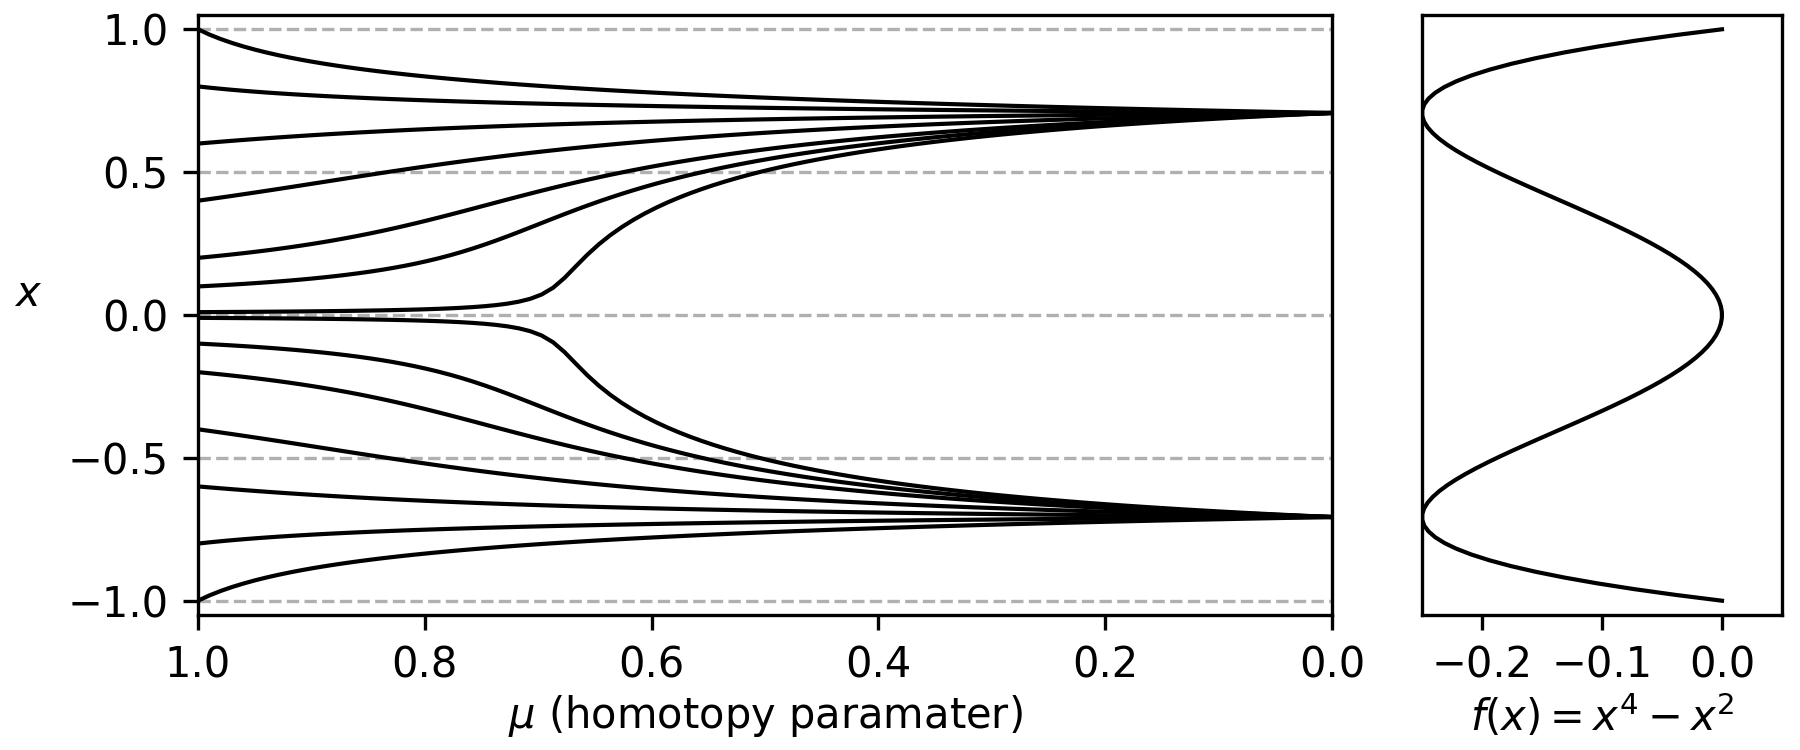
\includegraphics[width=\textwidth]{./figs/chap2/paths.png}
  \caption{Solution curves of $H(x,x_0,\mu) = 0$ (left side of figure) for
    different values of $x_0$.  The paths begin at $\mu=1$ and converge to the
    local minimizers at $\mu=0$.  The function to be minimized is plotted on the
    right-side of the figure.\label{fig:zc}}
\end{figure}

\subsection{Review of convergence theory for homotopy methods}

The path-following process described above, while intuitive, is not guaranteed
to succeed.  In particular, it is not clear that $\nabla_q H$ remains
non-singular along the path.  A poor choice of $G(q)$ may produce a level set
$H(q,q_0,\mu) = 0$ with an intersection, where $\nabla_q H$ is singluar and the path
bifurcates.  The Jacobian will also become rank deficient at so-called turning
points, where following the path from $\mu=1$ to $\mu=0$ requires $\mu$ to
increase at some point.  Finally, the path may diverge before reaching
$\mu=0$.

Many of the potential issues with the path-following approach can be avoided if
we place some conditions on the map $H$.  These conditions are described in the
theorem below, which has been adapted from~\cite{watson_2002} to the present
context.

\begin{theorem}\label{thm:homotopy}
  Assume the following conditions hold:
  \begin{itemize}
  \item $G : \mathbb{R}^{N} \times \mathbb{R}^{N} \rightarrow \mathbb{R}^{N}$ is
    a $C^2$ map, and $q=q_0$ is the unique solution to $G(q,q_0) = 0$;    
  \item $F :\mathbb{R}^{N} \rightarrow \mathbb{R}^{N}$, the first-order
    optimality residual given by \eqref{eq:opt00x}, is a $C^2$ map;
  \item For the homotopy map $H$ defined by \eqref{eq:homotopy}, the Jacobian 
  \begin{equation*}
    \nabla H \equiv \begin{bmatrix} \nabla_q H & \nabla_{q_0} H & \nabla_\mu
    H \end{bmatrix}
  \end{equation*}   
     is full-rank on the zero set $X \equiv \{(q,q_0,\mu) |
    H(q,q_0,\mu) = 0 \}$.
  \end{itemize}
  Then, for almost all $q_0 \in \mathbb{R}^{N}$, there exists a zero curve of
  $H$ starting from $q=q_0$ at $\mu=1$ along which the Jacobian $\nabla H$ has
  full rank.  Furthermore, if the set $X$ is bounded, then the path includes a
  point $(q,q_0,\mu) = (q^*,q_0,0)$, \ie, where $H(q^{*},q_0,0) = F(q^{*}) = 0$.
  Finally, if the Jacobian $\nabla_q F$ is invertible at $q^{*}$, the path has
  finite arc length.
\end{theorem}

Theorem~\ref{thm:homotopy} is a powerful result.  It implies that, for almost
all choices of $q_0$, there exists a path from $q=q_0$ at $\mu=1$ to a point
$q=q^*$ at $\mu=0$ that satisfies $F(q^*) = 0$, and along this path the Jacobian
is full-rank.  The phrase \emph{``almost all choices of $q_0$''} means that the
set of points for which there is no path has measure zero.

The drawback of Theorem~\ref{thm:homotopy} is that its assumptions, with the
exception of the first, are difficult to guarantee or verify in
practice\footnote{The first condition requires $G$ to be sufficiently smooth and
  have $q_0$ as its only solution; as we show in Section~\ref{sec:map}, it is
  straightforward to construct such a map.}.  The second condition, which cannot
be relaxed~\cite{watson_2002}, implies that the objective and constraints are
$C^3$.  While this level of smoothness exists for many engineering problems, it
is certainly not true in general.  The third assumption means that $H$ is
\emph{transversal to zero} for each choice of $q_0$, which can be verified for
simple problems, but may be difficult to determine for complex engineering
design problems.  Finally, as Watson points out in~\cite{watson_2002}, the
assumptions on the boundedness of the path and the invertibility of $\nabla_q F$
at $q^{*}$ are the most difficult to verify, since, taken together with the
other conditions, they imply the exsistence of a solution to $F(q) = 0$.

Despite the potential difficulty of guaranteeing the assumptions of
Theorem~\ref{thm:homotopy}, the theorem hints at the robustness of the homotopy
approach, and this is corroborated by our experience.

\subsection{Homotopy map for constrained optimization}\label{sec:map}

For this work we use the convex homotopy defined by \eqref{eq:homotopy},
therefore we need only define $G(q,q_0)$.  Similar to the unconstrained case, we
could use a map of the form
\begin{equation*}
  G(q,q_0) = q - q_0,
\end{equation*}
where $q_0 = \begin{bmatrix} x_0^T & s_0^T & \lambda_{h0}^T &  \lambda_{g0}^T \end{bmatrix}^T$.  However, this map produces a
positive-definite (diagonal) Jacobian $\nabla_q G$, which would be inconsistent
with the inertia of the Jacobian $\nabla_q F$ at a local solution to
\eqref{eq:opt00x}~\cite{Nocedal2006NO}.  Instead, we adopt the map
\begin{equation*}
  G(q,q_0) \equiv \begin{bmatrix}
    (x - x_0)^T &
    (s - s_0)^T &
    -\lambda_h^T & 
    -\lambda_g^T
  \end{bmatrix}^T, 
\end{equation*}
for which $q_0 = \begin{bmatrix} x_0^T & s_0^T & 0^T & 0^T \end{bmatrix}$.
We note that $G(q,q_0)$ satisfies the requirements of
Theorem~\ref{thm:homotopy}. 

For future reference, we restate the homotopy map that we use for solving the
first-order necessary conditions in this work:
\begin{equation}\label{eq:homo0}
    H(q, q_0, \mu) = (1-\mu)
    \begin{bmatrix}
      \nabla_x f(x) +   \lambda_h^T \nabla_x h(x)  +  \lambda_g^T \nabla_x g(x) \\
      -\mathsf{S}\mathsf{\Lambda_g} e \\
      h(x) \\
      g(x) - s 
    \end{bmatrix}
    + \mu
    \begin{bmatrix}
      x - x_0 \\
      s - s_0 \\
      -\lambda_h \\
      -\lambda_g
    \end{bmatrix}.
\end{equation}

\begin{remark}
  The homotopy map \eqref{eq:homo0} can be used to identify stationary points of
  $F(q)$, but it cannot, on its own, ensure that $s_i \geq 0$ and $\lambda_{i}
  \leq 0$.  We use safeguards to ensure the correct signs for the slacks and
  inequality multipliers; see Section~\ref{sec:fraction}.
\end{remark}

The homotopy map \eqref{eq:homo0} is favorable in the context of optimization
for several reasons.  First, the term $\mu(x-x_0)$ helps to address nonconvexity
by adding a positive diagonal matrix to the Lagrangian Hessian during the early
stages of convergence.  Furthermore, the term $\mu(s - s_0) \ \text{with} \ s_0 > 0$ generates a path
that remains feasible with respect to the slack boundaries $s>0$.  Finally, the
terms $-\mu\lambda_{h} \ \text{and} \ -\mu\lambda_{g}$ improve the conditioning of the
KKT matrix; even when the constraint Jacobian is rank deficient the homotopy map
will remain invertible for $\mu > 0$.

\section{Predictor-Corrector Path-following Algorithm}\label{sec:pc}
The theory presented in Section~\ref{sec:homotopy} tells us when a path exists
between $q_0$ and a solution to $F(q)$, but it does not tell us how to traverse
such a path in an efficient manner.  In this section we describe the modified
predictor-corrector algorithm~\cite{allgower_georg_1993} used to trace the
zero-curve of the homotopy map.

\subsection{Overview}

Figure \ref{fig:exact_pc}  illustrates the predictor and corrector phases at iteration
$k$ when exact linear and nonlinear solutions are possible.  
The iteration begins by computing a tangent to the path,
$q_{k+1}'$, and using this tangent to predict the next point on the path.
Subsequently, the homotopy parameter $\mu$ is fixed and a correction is found
that gives a root of the homotopy.  This cycle is repeated until $\mu <
\epsilon_\mu$, where $\epsilon_\mu > 0$ is a specificed tolerance.  Once $\mu$ is
sufficiently close to zero an approximate solution of the primal-dual system is
recovered.

\begin{remark}
  We use a default value of $\epsilon_\mu = 10^{-9}$ in our algorithm, which we
  have found works well for most problems; however, for difficult problems, \eg,
  with rank-deficient constraint Jacobians, it may be necessary to use larger
  thresholds.  For example, we use $\epsilon_\mu = 10^{-6}$ in the structural
  optimization problem presented in Chapter~\ref{sec:fstopo2}.
\end{remark}

In practice, the linear and nonlinear subproblems cannot be solved exactly.  Thus, the true situation is more like that in Figure \ref{fig:inexact_pc}, which depicts the path-following algorithm when inexact solutions are obtained.  These inexact solutions are discussed in the following high-level description of the predictor and corrector phases.  


\begin{figure}[tbp]
  \centering
  \subfloat[exact solves \label{fig:exact_pc}]{
    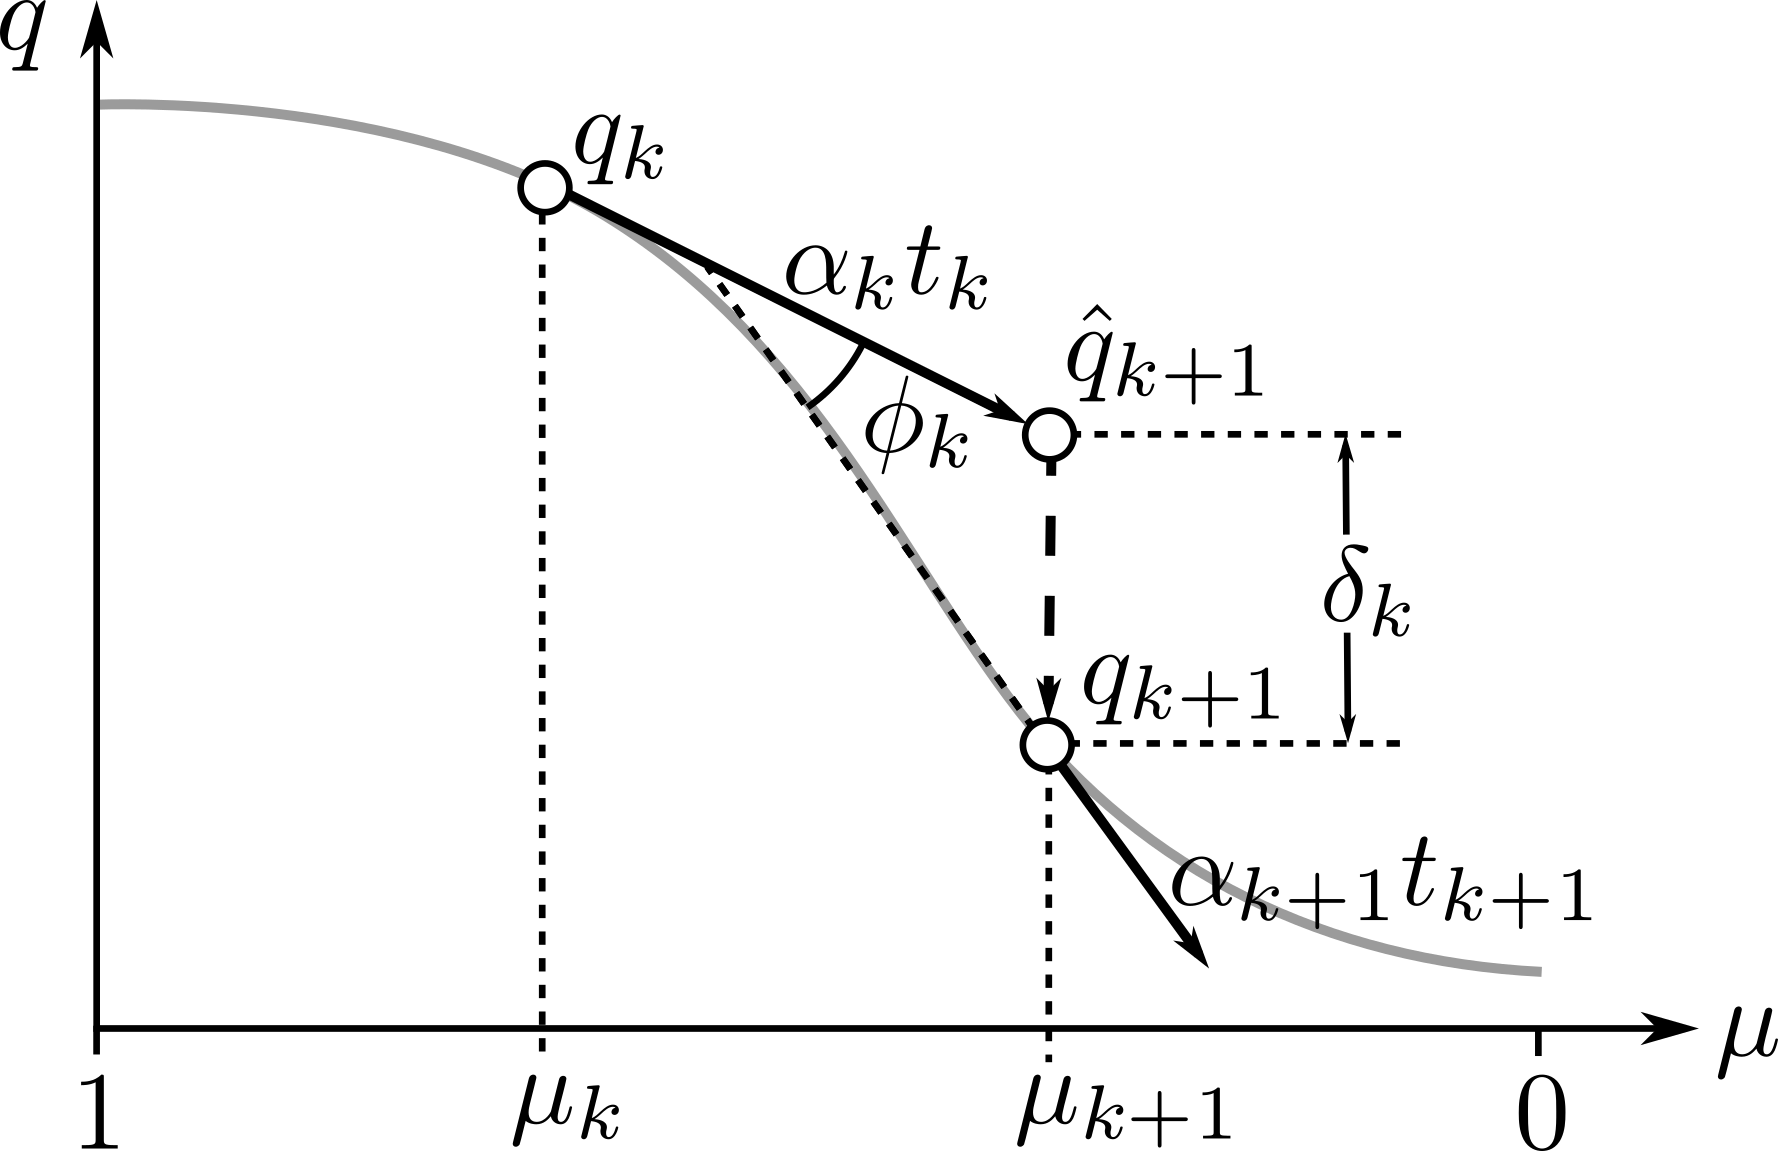
\includegraphics[width=0.6\linewidth]{figs/chap2/exact_pc.png} }
  \hspace{3em} 
  \subfloat[inexact solves\label{fig:inexact_pc}]{
  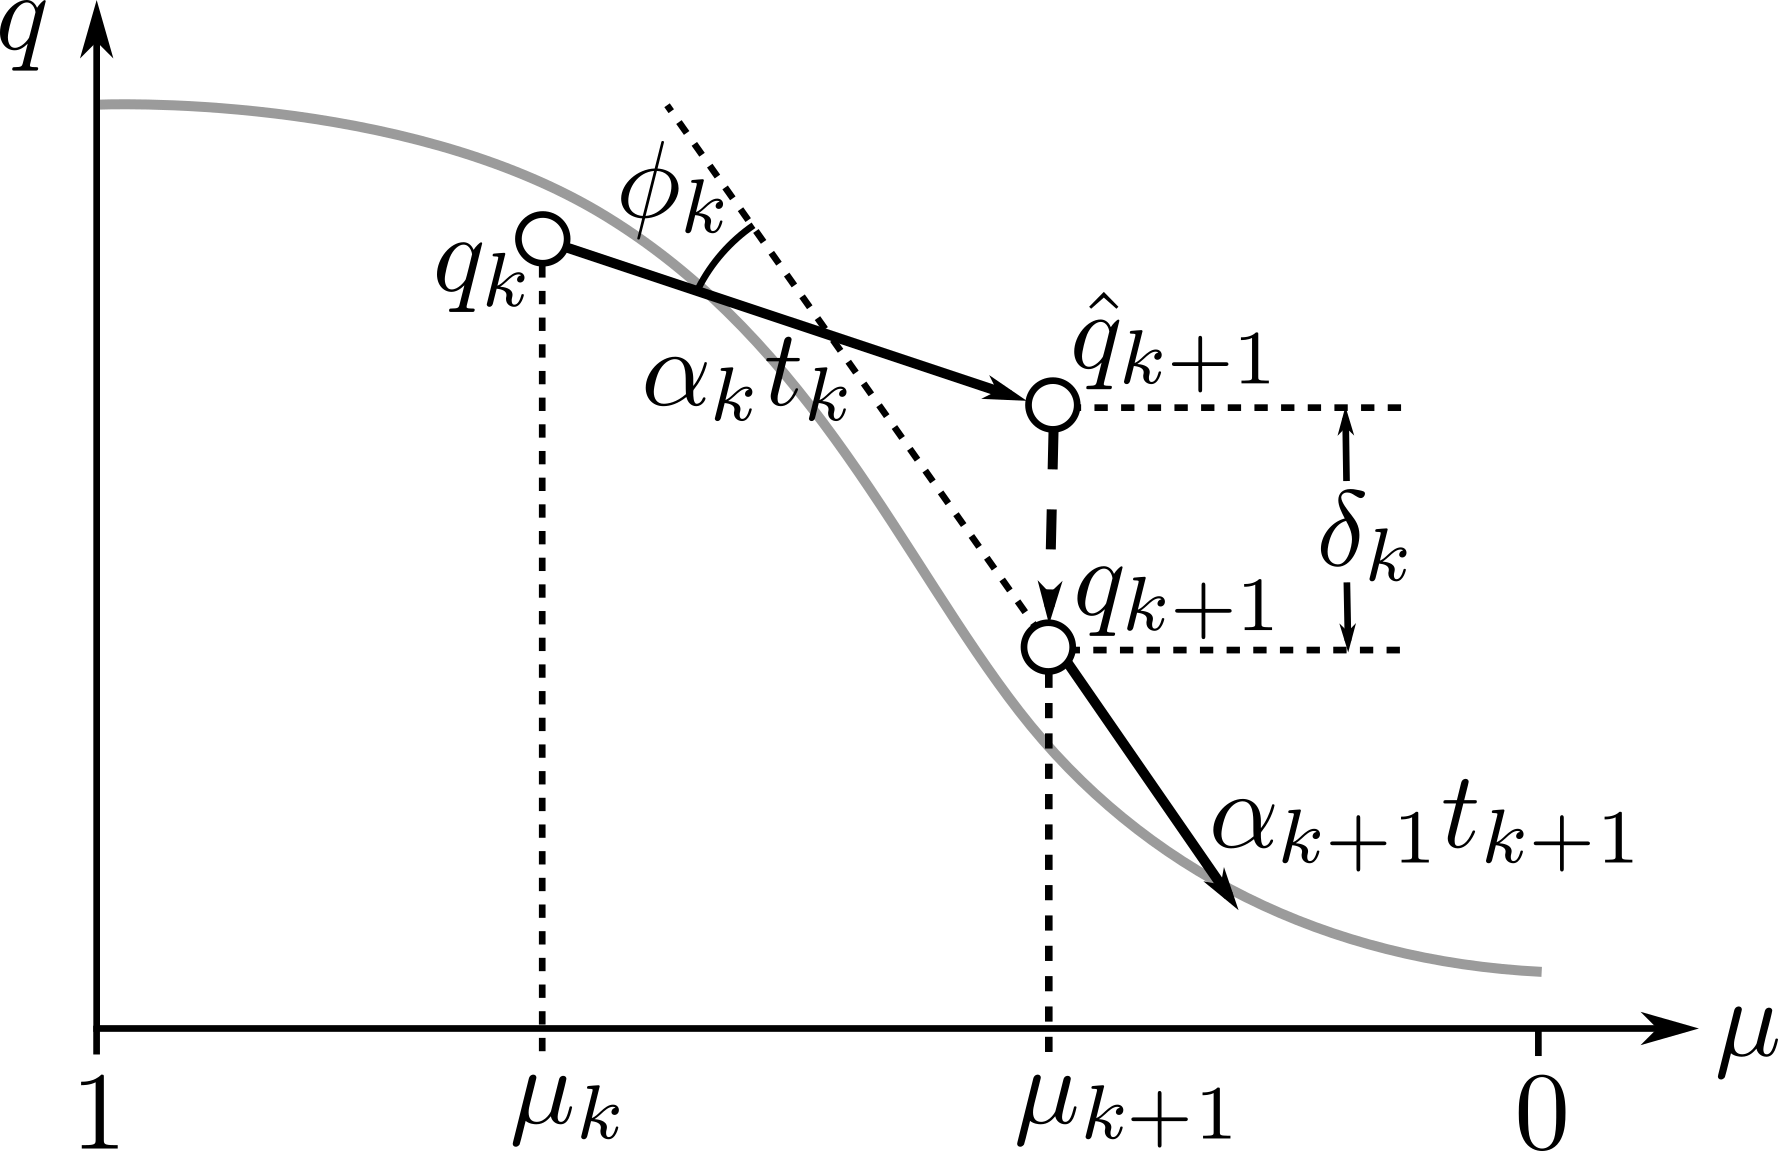
\includegraphics[width=0.6\linewidth]{figs/chap2/inexact_pc.png}
  }
 \caption{ Figure~\ref{fig:exact_pc} illustrates the predictor-corrector algorithm in the case that exact solves are used, while Figure~\ref{fig:inexact_pc} depicts the situation when inexact solves are used. \label{fig:pc}}   
\end{figure}


\begin{description}\label{sec:desp}

  \item[Predictor:] During the predictor phase we first need to compute an
    approximate tangent direction $q' = dq/d\mu$, which is defined by taking the
    total derivative of $H(q,q_0,\mu) = 0$ with respect to $\mu$, \ie by applying the
    implicit function theorem:
    \begin{equation}
      \left(\nabla_q H\right)_{k} q_{k}' = -\nabla_\mu H_{k} = F(q_k)  - G(q_k,q_0)
      \label{eq:predictorx}
    \end{equation}
    where $\nabla_q H$ and $\nabla_\mu H$ are evaluated at $q_k$, the previous
    homotopy iterate.  In practice, we solve \eqref{eq:predictorx} inexactly
    using a preconditioned Krylov iterative method.  That is, we find a $q_{k}'$
    that satisfies
    \begin{equation*}
      \lVert \left(\nabla_q H\right)_{k} q_{k}' - F(q_k) + G(q_k,q_0) \rVert
      \leq \tau \lVert F(q_k)  - G(q_k,q_0) \rVert,
    \end{equation*}
    where $\tau \in [0,1)$ is the desired relative tolerance.  Further details
      on the inexact solution of \eqref{eq:predictorx} are provided in
      Chapter~\ref{chap:linsys}.
    
    After (inexactly) solving \eqref{eq:predictorx} for $q_{k}'$, the predictor
    step is given by
    \begin{equation}\label{eq:pred}
      \begin{bmatrix}
        \hat{q}_{k+1} \\ \mu_{k+1} 
      \end{bmatrix} 
      = \begin{bmatrix}
        q_k \\ \mu_k 
      \end{bmatrix}      
      + \alpha_{k} t_{k},
    \end{equation}
    where $\alpha_{k}$ is the step length taken along the tangent direction at
    iteration $k$ (see Section~\ref{sec:step}), and $t_k$ is the normalized
    tangent given by
    \begin{equation}\label{eq:tk}
      t_{k} \equiv \frac{1}{\sqrt{\|q_{k}'\|^2 + 1}} \begin{bmatrix} -q_k'
        \\ -1 \end{bmatrix}.
    \end{equation}
    Note that the negative signs in the definition of $t_k$ account for
    decreasing $\mu$ as the path moves from $\mu=1$ to $\mu <
\epsilon_\mu$.

  \item[Corrector:] In the corrector phase, we fix the homotopy parameter
    at $\mu=\mu_{k+1}$ based on the predictor, and use a Newton-Krylov method to
    inexactly solve $H(q_{k+1},q_0,\mu_{k+1}) = 0$.  This has the effect of
    ``correcting'' $\hat{q}_{k+1}$ to be closer to the path.  More precisely,
    we seek $q_{k+1}$ that reduces the relative residual below some tolerance:
    \begin{equation}\label{eq:cornt}
      \lVert H(q_{k+1},q_0,\mu_{k+1}) \rVert \leq
      \epsilon_H \lVert H(\hat{q}_{k+1},q_0,\mu_{k+1}) \rVert.
    \end{equation}
    A loose relative tolerance of $\epsilon_H \in [0.1,0.5]$ is used for
    homotopy parameter values $\mu > 0$ to avoid oversolving the corrector step.
    Once the algorithm reaches $\mu \leq \epsilon_\mu$, the tolerance is tightened to the
    user-specified value for the first-order necessary conditions.
    
    At each Newton subiteration within the corrector, we must solve a linear
    system of the form
    \begin{equation}\label{eq:cor}
      \left(\nabla_q H \right)_{k+1} \Delta q_{k+1} = -H,
    \end{equation}
    for $\Delta q_{k+1}$, where $(\nabla_q H)_{k+1}$ and $H_{k+1}$ are evaluated
    at $\mu_{k+1}$ and the current estimate for $q_{k+1}$.  The Jacobian,
    $\nabla_q H$, that appears in \eqref{eq:cor} also appears in
    \eqref{eq:predictorx} during the predictor phase; again, further details
    regarding the solution of the linear systems that involve $\nabla_q H$ are
    provided in Chapter~\ref{chap:linsys}.

\end{description}

\begin{remark}
  The above predictor-corrector approach is a classical  embedding \\
  method~\cite{allgower_georg_1993}, since the solution path is assumed to be
  parameterized by $\mu$; that is, the path has the form $(q(\mu),\mu)$.  This
  type of method cannot handle folds, or turning points, where the path reverses
  direction with respect to $\mu$ and the Jacobian $\nabla_q H$ becomes
  singular.  Problems for which such turning points arise can be handled using
  more advanced predictor-corrector algorithms; see, for
  example,~\cite{walker:1999}.
\end{remark}

\subsection{Implementation details}

\subsubsection{Adaptive step-size control}\label{sec:step}

The step length $\alpha$ along the tangent direction is calculated using the
asymptotic expansion method \cite{allgower3}, which we briefly review here.

At the first iteration of the predictor-corrector algorithm when $\mu=1$, a
conservative step length is used, \eg, $\alpha_0 = 0.05$.  Subsquent step
lengths are then determined adaptively using a scaling factor and a couple
safeguards on the maximum step size:
\begin{equation*}
  \alpha_{k} = \min\left( \sqrt{\|q_{k}'\|^2 + 1}\Delta \mu_{\max}, \alpha_{\max}, \alpha_{k-1}/\zeta_{k} \right),
\end{equation*}
where $\Delta \mu_{\max}$ is the maximum allowable change in $\mu$,
$\alpha_{\max}$ is allowable step size permitted by the fraction-to-the-boundary
rule (see Section~\ref{sec:fraction}), and the scaling factor for $\alpha_{k-1}$ is given by
\begin{equation*}
  \zeta_{k} \equiv \max\left( \sqrt{\delta_k/\delta_{\text{targ}}}, \phi_k / \phi_{\text{targ}} \right).
\end{equation*}

The scaling factor $\zeta_k$ is controlled by two quantities that measure how
nonlinear the path is, namely the previous corrector update size, $\delta_k$, and the angle
between successive tangents, $\phi_k$.  Referring to Figure~\ref{fig:pc}, the corrector
update size is the magnitude of the difference between the predictor step and
the corrector step:
\begin{equation}\label{eq:delta_k}
  \delta_k \equiv \| q_{k} - \hat{q}_{k} \|.
\end{equation}
A large value of $\delta_k$ indicates that the linear predictor does not
approximate the path well, so a smaller step size is warranted.  The angle
between the tangents is
\begin{equation}\label{eq:phi_k}
  \phi_k \equiv \arccos\left(t_{k+1}^T t_{k} \right).
\end{equation}
The angle $\phi_k$ is a measure of the curvature in the path, so a relatively
large value of $\phi_k$ also suggests that $\alpha_k$ should be reduced.  For
locally linear paths both $\delta_k$ and $\phi_k$ are zero, and the scaling
factor will lead to an unbounded $\alpha_k$; hence the need for the maximum
allowable step $\alpha_{\max}$.

\begin{remark}
  While the adaptive step-size control is automated, performance depends on the
  parameters $\alpha_0$, $\Delta \mu_{\max}$, $\delta_{\text{targ}}$ and
  $\phi_{\text{targ}}$.  The optimal choice for these parameters is problem
  dependent.
\end{remark}

\subsubsection{Safeguards on the slacks and inequality multipliers}\label{sec:fraction}
One of the differences between solving \eqref{eq:opt00x} and solving a generic
nonlinear system of equations is that the slacks and inequality multipliers must
remain nonnegative and nonpositive, respectively.  To cope with this additional
set of requirements, the following safeguards are implemented in the
predictor-corrector scheme.
\begin{itemize}
  \item During the predictor phase, the maximum allowable step size is bounded
    using a fraction-to-the-boundary-like rule~\cite{Nocedal2006NO} defined
    below.
  \begin{equation}\label{eq:f2b}
      \alpha_{\max} = \max\left\{
      \alpha \in (0,1] \;|\; s + \alpha s' \geq \tau_s .\right\}.
    \end{equation}
where $\tau_s = 10^{-6}$. The fraction-to-the-boundary rule we use is slightly 
different than~\cite{Nocedal2006NO} in that we use a fixed absolute value $\tau_s$ as the boundary 
instead of a fixed fraction boundary. 


%If a particular slack variable gets close to zero, that is, if 
%   \begin{equation*}
%   0 <  s \leq \tau_s, 
%   \end{equation*}
% then its value is frozen and it is excluded from the above
% calculation of $\alpha_{\max}$.

In addition, the following clipping rule to the slack variable: 
\begin{equation}\label{eq:sclip}
    s \leftarrow \max(s, \tau_s)
\end{equation}
is applied at two locations: at the very beginning to the initial 
slack $s_0$, and at the last point of the corrector phase. 

    The maximum step size is enforced for all variables, including the design
    variables $x$.  We have found that synchronizing the step size across the
    design, slack and multipliers improves the performance of the algorithm.
    
  \item After both the predictor and the corrector step,
  the inequality multipliers are clipped to
    ensure they remain non-positive:
    \begin{equation}\label{eq:lclip}
     \lambda_g \leftarrow \min(\lambda_g, 0)
    \end{equation}
      %\hat{\lambda}_{k+1} = \min(\lambda_{k} + \alpha_k (t_k)_{\lambda}, 0),

    where the $\min$ function in the above expression is to be
    interpreted elementwise.  
    %$(t_k)_{\lambda}$ denotes the multiplier component of the normalized tangent
\end{itemize}

While the slacks and inequality multipliers both have similar bound constraints, their treatment is
slightly different in the above safeguards.  Our motivation for bounding the
slacks away from zero, in both the predictor corrector phases, is to avoid
severe ill-conditioning in the system matrix and its preconditioner; see
Section~\ref{sec:matfreepc} for further details.  The inequality multipliers, in contrast,
do not lead to conditioning problems if they vanish, so we can clip the
multipliers to zero.

\subsection{Algorithm Summary}

With most of its elements described, we summarize the predictor-corrector method
in Algorithm~\ref{alg:pc}.  The solution of the tangent step,
line~\ref{line:tang}, and the solution of the Newton step, line
\ref{line:newton}, are the only components of the algorithm that require further
explanation.  Note that the initial tangent step line~\ref{line:tang0} is a linear system that 
is trivial to solve. % The solution of these linear systems is detailed in the next chapter.
\\
\LinesNumberedHidden
\begin{algorithm}[H]\setstretch{1.35}
\SetKwInOut{Input}{Input}
\SetKwInOut{Output}{Output}
\SetKwInOut{Parameter}{Parameters}
\SetKw{Break}{break}
\SetKw{Return}{return}
\SetEndCharOfAlgoLine{}
%\SetKwRepeat{Do}{do}{while} %

\Parameter{$K_{\max}$, $J_{\max}$, $\epsilon_F$, $\tau$, $\epsilon_H$, $\alpha_0$, $\delta_{\text{targ}}$, $\phi_{\text{targ}}$, $\Delta \mu_{\max}$}
\Input{$x_0$, $s_0$}
\Output{$q^{*} = \begin{bmatrix} x^{*T} & s^{*T} & \lambda_h^{*T} & \lambda_g^{*T}   \end{bmatrix}^T$, the solution of \eqref{eq:opt00x}}
\BlankLine
Clip $s_0$ if necessary: $s_0 \leftarrow \max(s_0,\tau_s)$  \\
Set $q_0 = \begin{bmatrix} x_0^T & s_0^T& 0^T & 0^T \end{bmatrix}$, $q  \leftarrow q_0 $  \\
compute state $u$,  adjoint $\psi$ for $q_0$ \\
\ShowLn
inexactly solve $\left(\nabla_q H\right)_{k} q_{k}' = - \nabla_\mu H_{k} $ \label{line:tang0}   
 for $q_{k}'$ to required tolerance $\tau$ \label{line:initPred} \\
compute the normalized tangent direction $t_{k}$ using \eqref{eq:tk} \\

\For{$k = 0,1,2,\ldots,K_{\max}$}{
 compute $\alpha_{k} (\alpha_0 \text{~if~} k\equiv0) = \min\left( \sqrt{\|q_{k}'\|^2 + 1}\Delta \mu_{\max}, \alpha_{\max}, \alpha_{k-1}/\zeta_{k} \right)$\\
  use \eqref{eq:pred} to update $\hat{q}_{k+1}$ and $\mu_{k+1}$\\
  clip $\lambda_{g, k+1}$ if necessary:  $\lambda_{g, k+1} = \min(\lambda_{g, k+1}, 0)$  \\
  update state $u$, adjoint $\psi$ at $\hat{q}_{k+1}$ \\
  set $q_{k+1} \leftarrow \hat{q}_{k+1}$\\
  
  \For{$j = 0,1,2,\ldots,J_{\max}$}{ 
%     \ShowLn
%      \lIf{$\| F(q_{k}) \| \leq \epsilon_{F} \|F(q_{0})\|$}
%     {\Break \Break}   %,  $s_{i} \geq 0$
     \lIf{$\lVert H(q_{k+1},q_0,\mu_{k+1}) \rVert \leq \epsilon_{H} \lVert
      H(\hat{q}_{k+1},q_0,\mu_{k+1}) \rVert$}{%
      \Break
    }
    \ShowLn
    inexactly solve $\left(\nabla_q H \right)_{k+1} \Delta q_{k+1} =
    -H_{k+1}$ for $\Delta q_{k+1}$ \label{line:newton} \\
    $q_{k+1} \leftarrow q_{k+1} + \Delta q_{k+1}$ \\
    update state $u$, adjoint $\psi$ at $q_{k+1}$ \\ 
  }
  \ShowLn
    \lIf{$\mu_{k} < \epsilon_{\mu}$}{\Return $q_{k}$} 
   % $\| F(q_{k}) \| \leq \epsilon_{F} \|F(q_{0})\|$,  $s_{i} \geq 0$ ,
   % and $\lambda_{i} \leq 0$
  \ShowLn
   inexactly solve $\left(\nabla_q H\right)_{k} q_{k}' = - \nabla_\mu H_{k}$
  for $q_{k}'$ to required tolerance $\tau$   \label{line:tang} \\
  compute the normalized tangent direction $t_{k}$ using \eqref{eq:tk} \\
  update $\delta_k$ and $\phi_{k}$ according to \eqref{eq:delta_k} and
  \eqref{eq:phi_k} \\
  compute the step scaling factor: $\zeta_{k} = \max\left( \sqrt{\delta_k/\delta_{\text{targ}}}, \phi_k / \phi_{\text{targ}} \right)$\\
%  compute $\alpha_{k} = \min\left( \sqrt{\|q_{k}'\|^2 + 1}\Delta \mu_{\max}, \alpha_{\max}, \alpha_{k-1}/\zeta_{k} \right)$\\
  clip if necessary: $s_{k+1} \leftarrow \max(s_{k+1},\tau_s)$ and
  $\lambda_{k+1} \leftarrow \min(\lambda_{k+1},0)$ \\
  % $k \leftarrow k+1$   $\lambda_{k+1}$ and $s_{k+1}$
  }
\caption{Inexact-Newton predictor-corrector algorithm for PDE-Constrained
  optimization.\label{alg:pc}}
\end{algorithm}

\newpage
%%%%%%%%%%%%%%%%%%%%%%%%%%%%%%
\section{Globalization Numerical Experiments}
In theory, Newton-based methods can successfully solve the first-order necessary optimality conditions, but cannot guarantee that the solution also satisfies the second-order sufficient optimality conditions. However, the added homotopy term in the homotopy map~\eqref{eq:homo0} functions like regularization to the optimization problem, thus enable the proposed algorithm a certain amount of non-convex handling capacity. To verify this quality, two numerical examples are tested: the first one is a 3D Sphere constrained problem with a linear objective, and the second one is an indefinite quadratic problem with bound constraints. The goal is to check whether the proposed algorithm can bypass local maximum points.  


\subsection{Sphere Problem Description}
The first test problem to verify RSNK's globalization performance has a linear objective and a feasible domain that is the inside of a sphere:
\begin{equation*}
\begin{aligned}
\underset{x, y, z} {\text{min}}  & \quad \quad x + y + z \\
   {\text{subject to}}  & \quad \quad x^2 + y^2 + z^2 \leq 3 \\
\end{aligned}
\end{equation*}

The solution to this problem is at $(-1,-1,-1)^T$. There is a local maximum point at $(1,1,1)^T$, where the 
first-order optimality condition (KKT condition) is also satisfied but not the second-order optimality condition. 
The presence of this local maximizer provides a test for the homotopy-based globalization algorithm.

\subsection{Sphere Problem Results}
To prove that the algorithm can bypass the local maximum, 100 random starting points around the local maximum $(1,1,1)^T$ where generating by adding Gaussian perturbations, $\Delta x_i \sim \mathcal{N}(0,0.1^2)$, to each coordinate. Figure~\ref{fig:sphere_100_start} shows 100 random initial points as blue circles and the exact solution as a red star; Figure~\ref{fig:sphere_100_end} shows the final iterates as blue circles and the exact solution as a red star. As can be seen, even when the 100 starting points are near the local maximizer, they all converge to the minimum point.  

 \begin{figure}[H]
  \centering
  \subfloat[100 Starting Points Around Local Maximum \label{fig:sphere_100_start}]{
  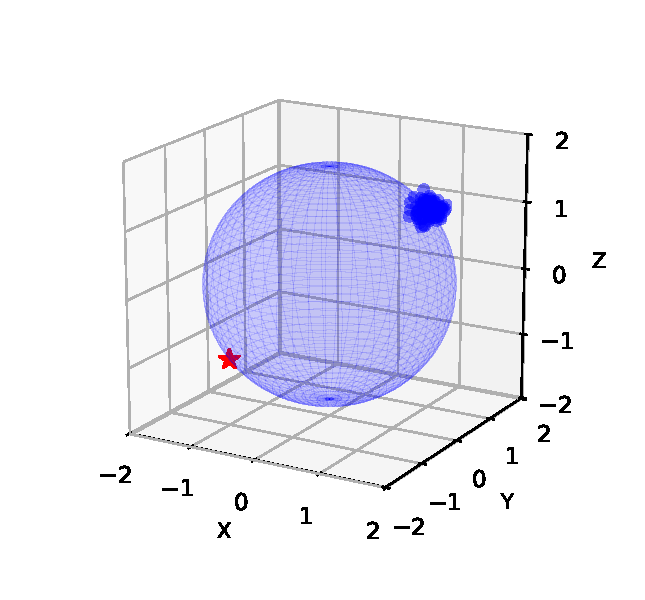
\includegraphics[clip, trim=20 10 20 30, width=0.7\columnwidth]{./figs/chap2/100_startingPoints.pdf} }  % 
  \hspace{1em}
   \subfloat[100 Ending Points \label{fig:sphere_100_end}]{
  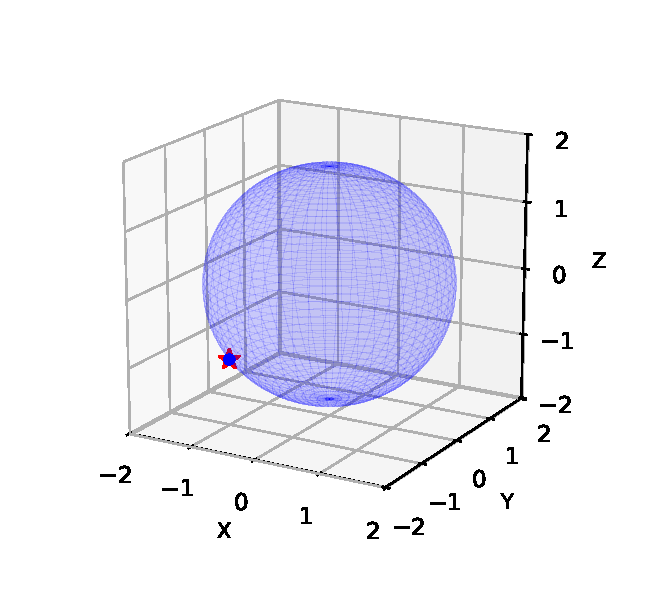
\includegraphics[clip, trim=20 10 20 30, width=0.7\columnwidth]{./figs/chap2/100_endingPoints.pdf} } 
   \caption{100 Starting and Ending Points \label{fig:sphere_100}}  
\end{figure}

 \begin{figure}[H]
  \centering
  \subfloat[1000 Starting Points \label{fig:sphere_1000_start}]{
  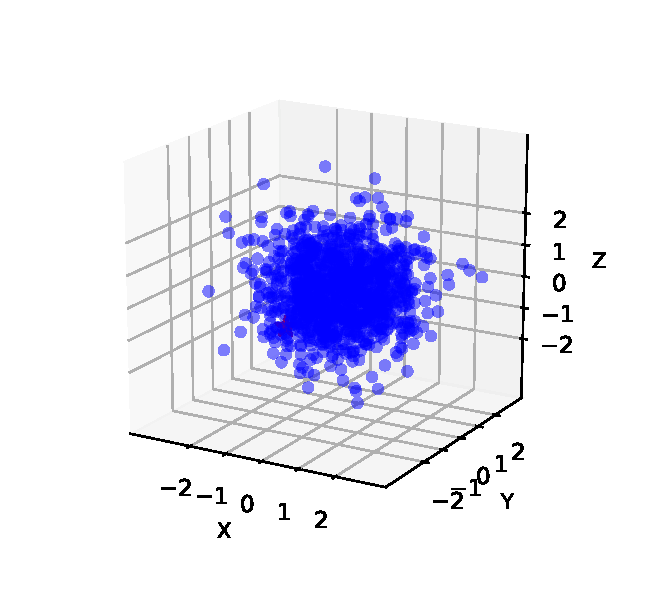
\includegraphics[clip, trim=20 10 20 40, width=0.7\columnwidth]{./figs/chap2/1000_startingPoints.pdf} } 
  \hspace{1em}
   \subfloat[1000 Ending Points  \label{fig:sphere_1000_end}]{
  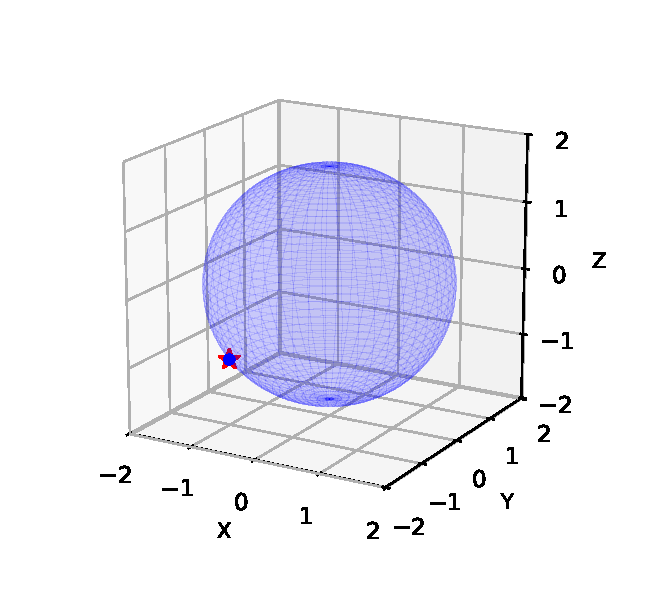
\includegraphics[clip, trim=20 10 20 30, width=0.7\columnwidth]{./figs/chap2/1000_endingPoints.pdf} } 
   \caption{1000 Starting and Ending Points \label{fig:sphere_1000}}  
\end{figure}

To further test the robustness of the globalization, we seeded the algorithm with 1000 initial guesses whose $x_0$ were drawn from a standard normal distribution. Figure~\ref{fig:sphere_1000_start} shows a scatter plot of these 1000 points.  All $x_0$ values converge to the local minimizer, as shown in Figure~\ref{fig:sphere_1000_end}.  

%%%%%%%%%%%%%%%%%%%%%%%%%%%%%%
\subsection{Non-convex Problem Description}
For our second numerical experiment, we consider the following simple 100-dimensional non-convex optimization problem:
\begin{equation*}
\begin{aligned}
&\underset{x \in R^{100}} {\text{min}}  
& &\phantom{-} \frac{1}{2}x^T \mat{Q} x \\
  & {\text{subject to}}
& &-1 \leq x_i \leq 1 \qquad \forall i = 1,2,\ldots,100, \\
\end{aligned}
\end{equation*}
where Q is a diagonal matrix whose entries are $-1$ or $1$ with uniform probability.
This problem is challenging for Newton-based optimization algorithms, which 
tends to locate stationery points  but cannot differentiate between 
minimizers or maximizers. As the objective function can be separated into 
individual dimensions, it is easy to see that 
valid minimizers for this problem have the following dependence on Q:
%\begin{equation}\label{eq:pattern}
%  x^{*} = \begin{bmatrix} 0 & \pm 1 & 0 & \cdots & 0 & \pm 1 \end{bmatrix}^{T}.
%\end{equation}
%where
\begin{equation}\label{eq:pattern2}
  \begin{gathered}
  x_i=0  \text{~if~}  \mat{Q}_{ii} = 1,  \\
  x_i = \pm 1  \text{~if~}  \mat{Q}_{ii} = -1.
  \end{gathered}
\end{equation}

We would like to investigate
the ability of the algorithm to avoid stationary points that are not local minimizers, 
\eg $x_i = 0$ 
when $\mat{Q}_{ii} = -1$ and $x_i = \pm 1$ when $\mat{Q}_{ii} = 1$.
Note that when $\mat{Q}_{ii} = 1$, the upper and lower bound $x_i = \pm 1$ are 
individual maximums where the gradient of the Lagrangian is zero in that dimension. 

\subsection{Non-convex Problem Results}
We ran the optimization algorithm on the non-conex problem with 1000 randomly generated Q matrices.
For each case, 
the arrangement of $1$ and $-1$ in $\mat{Q}$ is uniformly randomly generated; 
 the initial point $x_0$ is also generated randomly with uniform probability in the domain
  $\Omega = \{ x \in \mathbb{R}^{100} \; | \; -2 \leq x_i \leq 2 \}$.  We call a solution successful if 
  its pattern is exact as given by \eqref{eq:pattern2}.  Table~\ref{tab:success} lists the success rate for different 
  combinations of $\epsilon_{\text{krylov}}$ and $\epsilon_H$. 
Note that $\epsilon_{\text{krylov}}$ is the tolerance of the Krylov solver introduced in Chapter~\ref{2:krylov}; 
$\tau$ and $\epsilon_H$ are the tolerances for the predictor and the corrector step as explained in Description~\ref{sec:desp}. 
 
\begin{table}[H]
  \begin{center}
    \caption{Success Rate with Different Parameters \label{tab:success}}
  \begin{tabular}{ c   c   c   c  c  c  c  c }
  %\hline
 & \multicolumn{7}{  c   }{ $\epsilon_{\text{krylov}}$  } \\  \hline
 &   & $10^{-1}$  & $10^{-2} $     & $10^{-3} $    &  $10^{-4}$     & $ 10^{-5}$    & $10^{-6} $   \\  
\multirow{2}{*}{$\tau$ and $\epsilon_H$ } &  $10^{-1}$ & 51\%  &90.0\% &94.2\% &94.6\% &93.9\% & 93.8\%  \\
	               					      &  $ 10^{-2}$ & 47.2\%  &93.1\% &94.4\% &93.9\% &94.2\% &  94.5\%\\
   % \hline
  \end{tabular}
  \end{center}
\end{table}

As can be seen from Table~\ref{tab:success}, the robustness of the algorithm for handling non-convexity 
is obviously impacted by the tolerances, particularly $\epsilon_{\text{krylov}}$. The results show that 
$\epsilon_{\text{krylov}}$ has to be below $ 10^{-2}$
for effective non-convexity handling, and the predictor and corrector linear solve tolerance $\epsilon_H$ 
plays a smaller role than $\epsilon_{\text{krylov}}$.   
  
% \begin{figure}[tbp]
%  \centering
%  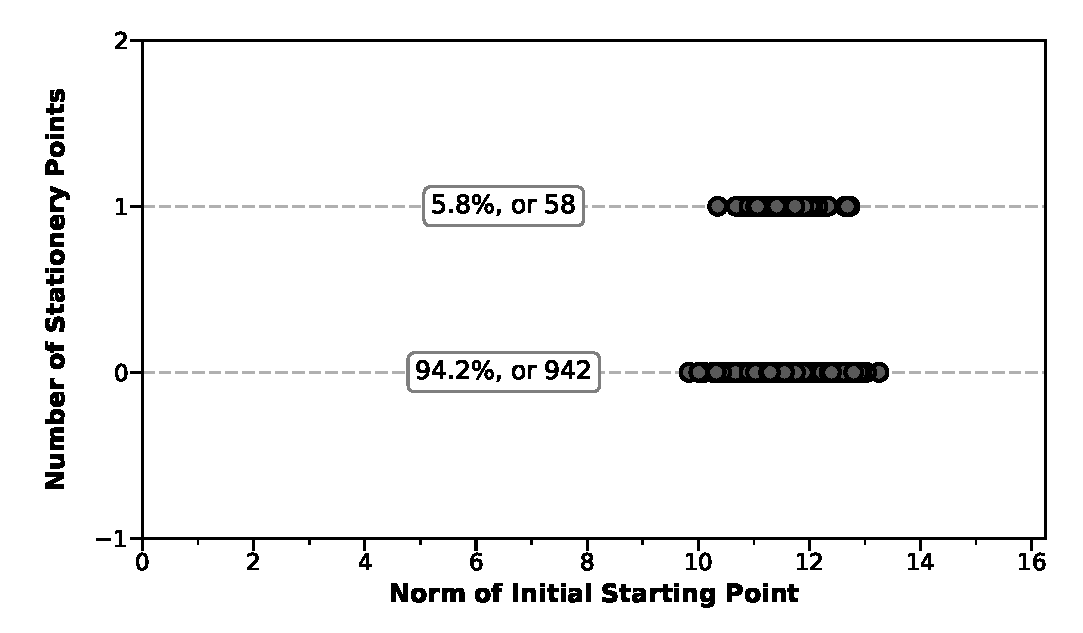
\includegraphics[clip,width=0.7\columnwidth]{./figs/chap4_test/nonconvex_1000_random.eps}%
%  \caption{Success Minimizers. \label{fig:nonconvex}}
%\end{figure}   
  
%\textbf{  I would delete 3.6 and this paragraph.  Alternatively, you could have a table that shows the percentage for each failed dimension. (I have never liked Fig. 3.6, probably because the norm of the initial starting point is not very useful predictor). }
  
  
The results show that the optimization method can start from infeasible points, and can handle certain 
amount of nonconvexity.  Admittedly, this nonconvex test problem is rather simple, with no complexities like bad-scaling, ill-conditioning included. However, the focus is solely to see whether the added regularization from the homotopy term can help 
Newton's method bypass local maximizers and saddle points.  Further work is needed to determine when the problem demands 
tighter tolerances and how to detect and handle nonnegative curvature.  


Typical optimization convergence plots are provided in Figure~\ref{fig:nc_converg}. Figure~\ref{fig:ncmu} 
shows the absolute optimality, complementarity and feasibility at each homotopy iteration of different $\mu$. 
Note that for simplicity, only the predictor points are displayed when $\mu \geq \epsilon_{\mu}$, 
while the corrector points are displayed for $\mu < \epsilon_{\mu}$.
Figure~\ref{fig:nccpu} shows convergence criteria with respect to  CPU time. 
These convergence plots indicate that, at least asymptotically, superlinear convergence is maintained by the algorithm.

\begin{figure}[tbp]
  \centering
  \subfloat[Convergence vs. $\mu$ \label{fig:ncmu}]{
   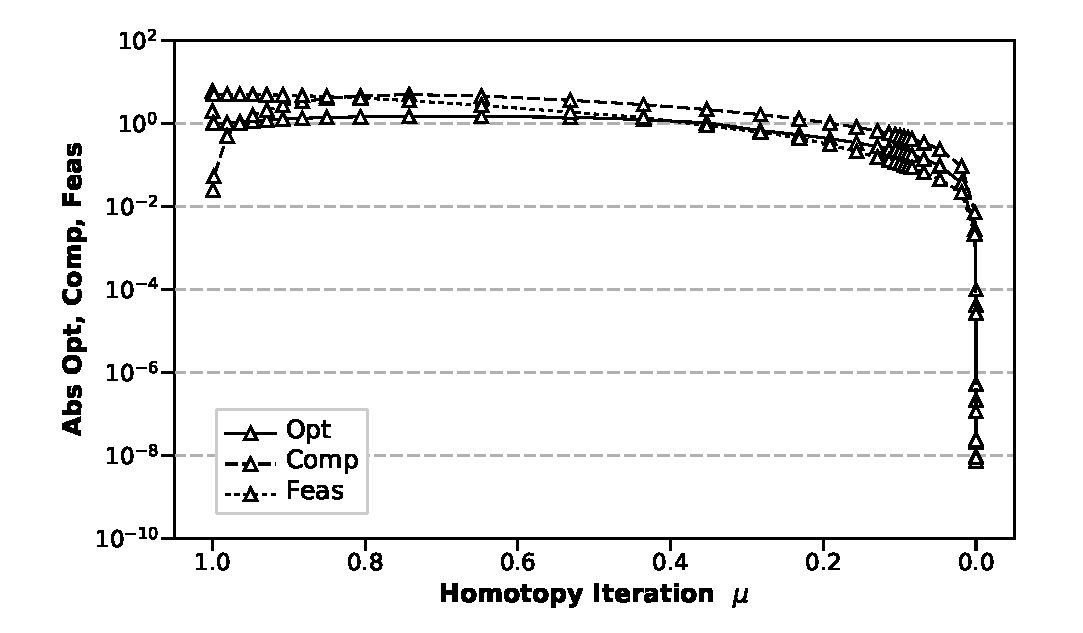
\includegraphics[clip,width=0.7\linewidth]{./figs/chap4_test/nonconvex_mu.eps} }
   \hspace{1em}
   \subfloat[Convergence vs. CPU time \label{fig:nccpu}]{
   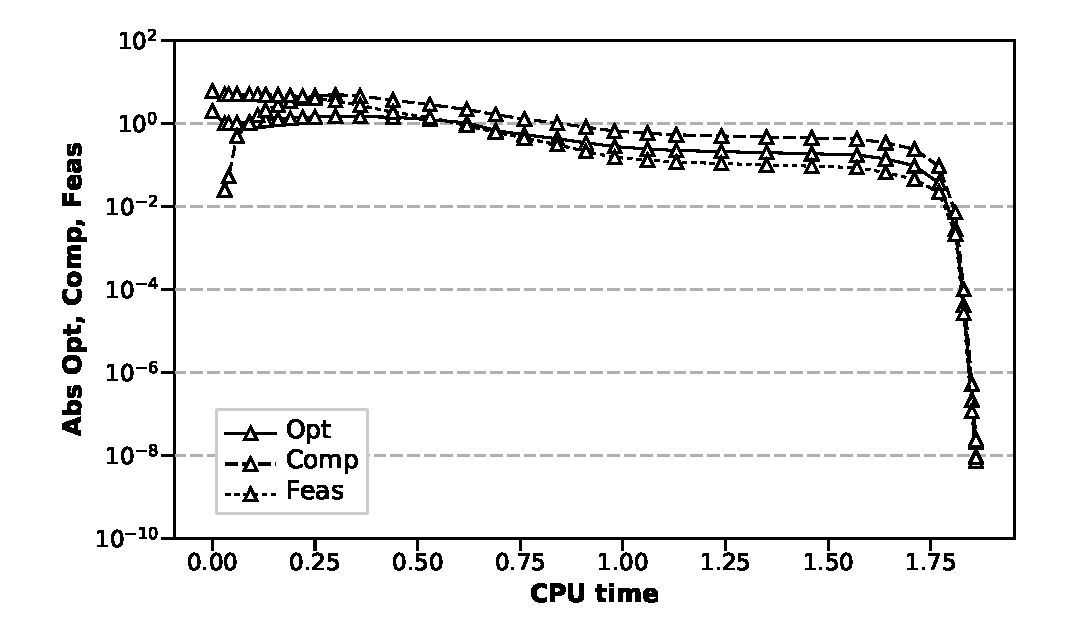
\includegraphics[clip,width=0.7\linewidth]{./figs/chap4_test/nonconvex_cpu.eps} }
   \caption{Typical Convergence Plots in $1000$ Random Cases \label{fig:nc_converg}}
\end{figure}

%\begin{remark}
% The parameters $\alpha_0$, $\delta_{\text{targ}}$, $\phi_{\text{targ}}$, and
%  $\Delta \mu_{\max}$ all play a role in the ability of Algorithm~\ref{alg:pc}
%  to handle nonconvex objectives.  If these parameters are set too agressively,
%  then the algorithm may move off the homotopy level-set and converge to a local
%  maximizer or saddle, even for the simple problem considered here.
%  \padd{I think this Remark should be removed now. As we've provided the influence of 
%  Krylov tolerance and inner tolerance on the success rate. }
%\end{remark}


 
%%%%%%%%%%%%%%%%%%%%%%%%%%%%%%%%%%%%%%%%%%%%%%%%%%%%%%%%%%%%%%%%%%% 
%                                                                 %
%                            CHAPTER TWO                         %
%                                                                 %
%%%%%%%%%%%%%%%%%%%%%%%%%%%%%%%%%%%%%%%%%%%%%%%%%%%%%%%%%%%%%%%%%%% 
 
\chapter{HOMOTOPY-BASED GLOBALIZATION}

\section{Homotopy-based Globalization}\label{sec:homotopy}
Homotopy methods are robust, numerically stable, and globally convergent methods
for solving nonlinear algebraic equations; see, for example,
\cite{allgower_georg_1993} and \cite{Watson_1989}.  Our interest in these
methods began as a means of globalizing difficult computational aerodynamics
problems~\cite{hicken:cfd2009, hicken:cfd2011b, Brown_2016}, but globally
convergent probability-one homotopy methods have also been successfully applied
to solve engineering optimization problems.  Watson~\cite{Watson_2001} reviewed
and developed the general convergence theory for nonlinear optimization
problems, including unconstrained, bound-constrained, linear and nonlinear
inequality constrained convex cases.  He also discussed the extension of the
theory to nonconvex problems, although the convergence theory for equality
constraints remains an open problem.  More recently, Huang
\etal~\cite{huang_2012pc} transformed a general nonlinear optimization with
equality and inequality into an inequality-only problem, and used a
predictor-corrector method to track the homotopy interior-point map using the
conjugate gradient method. While their method achieves global linear convergence
under the normal cone condition, it is limited to convex objective and
constraint functions.

\subsection{Example}

Conceptually, the idea of homotopy methods is easy to understand. To find the
solution of a difficult nonlinear equation, $F(q)=0$, a homotopy map is
constructed that connects the target problem to an easy-to-solve problem via a
parameter.  For example, a convex homotopy map $H : \mathbb{R}^N \times
\mathbb{R}^{N} \times [0,1) \rightarrow \mathbb{R}^N$ is given by
\begin{equation}\label{eq:homotopy}
H(q, q_0, \mu) = (1-\mu) F(q) + \mu G(q,q_0),\quad 0 \leq \mu \leq 1,
\end{equation}
where $\mu$ is the homotopy parameter, and $G : \mathbb{R}^N\times\mathbb{R}^{N}
\rightarrow \mathbb{R}^N$ is chosen such that $G(q,q_0)=0$ is easy to solve and
has the solution $q=q_0$.  Formally, a homotopy is a continuous map from the
interval $[0,1]$ into a function space.

We will use a simple, unconstrained optimization example to illustrate the
homotopy idea. Consider the problem
\begin{equation*}
\min_x  \quad  f(x) = x^4 - x^2.
\end{equation*}
The first-order optimality condition for this problem is given by (identifying
$q$ with $x$ here)
\begin{equation*}
F(x) = \nabla_x f(x) = 2x(2x^2 - 1) = 0.
\end{equation*}
It is easy to see that there are three stationary points; a local maximizer at
$x=0$ and two local/global minimizers at $x=\pm 1/\sqrt{2}$.  Newton's method
may converge to any of these stationary points depending on the initial guess
$x_0$, so we need some way to avoid the local maximizer at $x=0$.

Now, consider the simple problem $\min_x \; \frac{1}{2}(x - x_0)^2$, whose
first-order optimality is given by
\begin{equation*}
G(x,x_0) = x - x_0 = 0.
\end{equation*}
This has the obvious solution $x=x_0$.  We can take advantage of this simple
optimization problem by constructing a convex homotopy that combines $F(x)$ and
$G(x,x_0)$ as follows:
\begin{equation*}
  H(x, x_0, \mu) = (1-\mu) F(x) + \mu G(x, x_0) = (1 - \mu) 2x(2x^2 -1) + \mu (x
  - x_0).
\end{equation*}
Next, we trace out the set of solutions corresponding to $H(x,x_0,\mu)=0$ from
$\mu=1$ to $\mu=0$.  Starting at $\mu=1$ we have the solution $x=x_0$.  If we
change the value of $\mu$ slightly to $\mu = 1 - \Delta \mu$, then, for $\Delta
\mu$ sufficiently small and by continuity, $x_0$ should remain in the basin of
attraction for Newton's method applied to $H(x, x_0, 1-\Delta \mu)=0$.  The
solution at $\mu= 1 - \Delta \mu$ can then be used as an initial guess for the
next value of $\mu$, and so on, until we reach $\mu = 0$.  Example solution
paths for this process are illustrated in Figure~\ref{fig:zc} starting from
distinct $x_0$.  Notice that all paths converge to the local minimizers, even
those that begin near the maximizer $x=0$.

\begin{figure}[t]
  \centering
  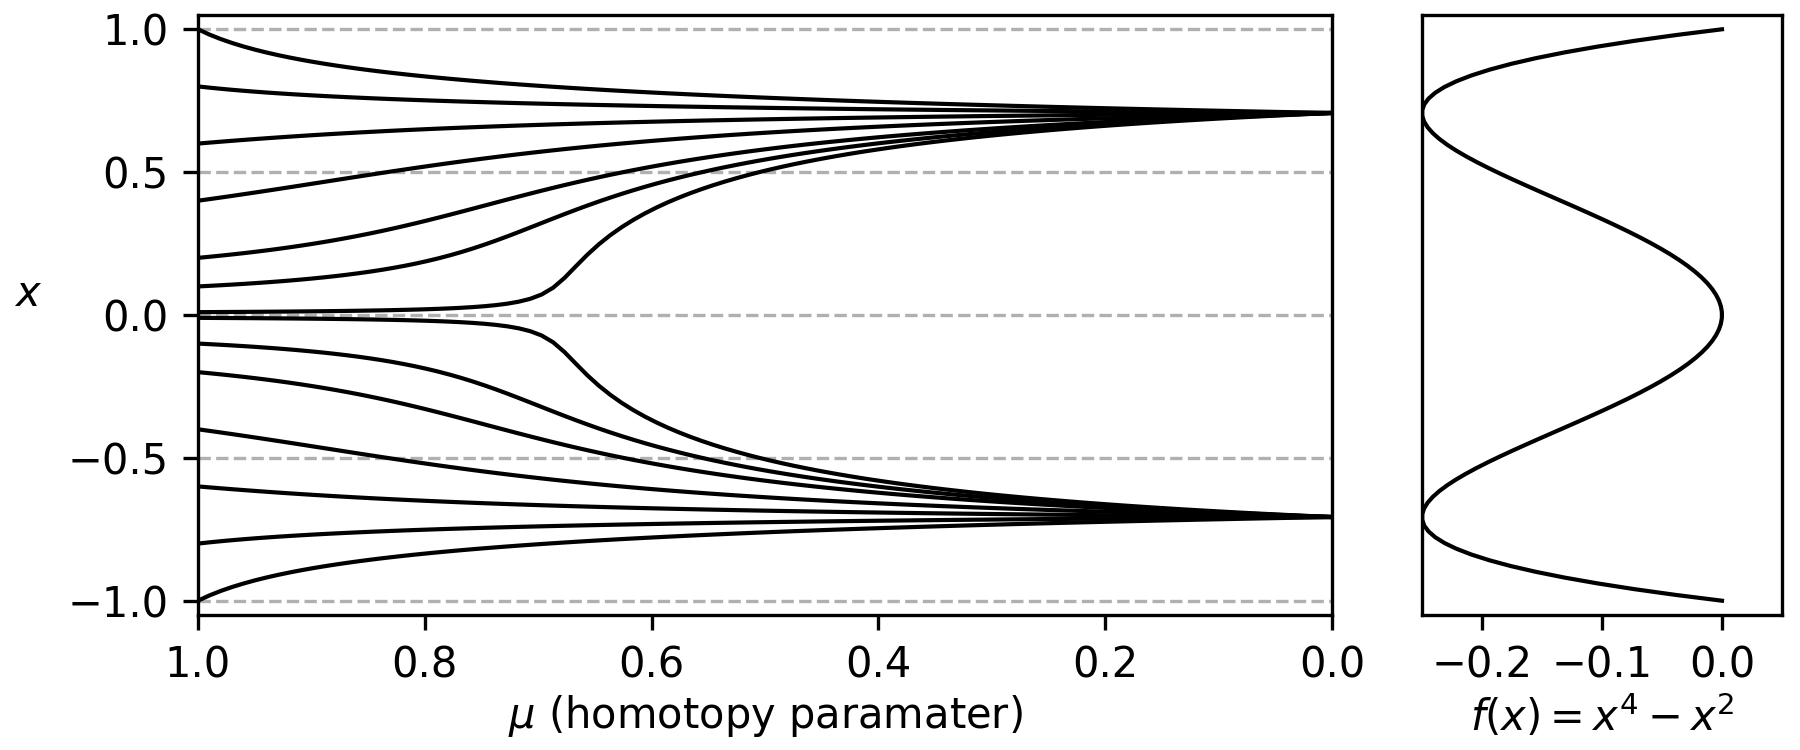
\includegraphics[width=\textwidth]{./figs/chap2/paths.png}
  \caption{Solution curves of $H(x,x_0,\mu) = 0$ (left side of figure) for
    different values of $x_0$.  The paths begin at $\mu=1$ and converge to the
    local minimizers at $\mu=0$.  The function to be minimized is plotted on the
    right-side of the figure.\label{fig:zc}}
\end{figure}

\subsection{Review of convergence theory for homotopy methods}

The path-following process described above, while intuitive, is not guaranteed
to succeed.  In particular, it is not clear that $\nabla_q H$ remains
non-singular along the path.  A poor choice of $G(q)$ may produce a level set
$H(q,q_0,\mu) = 0$ with an intersection, where $\nabla_q H$ is singluar and the path
bifurcates.  The Jacobian will also become rank deficient at so-called turning
points, where following the path from $\mu=1$ to $\mu=0$ requires $\mu$ to
increase at some point.  Finally, the path may diverge before reaching
$\mu=0$.

Many of the potential issues with the path-following approach can be avoided if
we place some conditions on the map $H$.  These conditions are described in the
theorem below, which has been adapted from~\cite{watson_2002} to the present
context.

\begin{theorem}\label{thm:homotopy}
  Assume the following conditions hold:
  \begin{itemize}
  \item $G : \mathbb{R}^{N} \times \mathbb{R}^{N} \rightarrow \mathbb{R}^{N}$ is
    a $C^2$ map, and $q=q_0$ is the unique solution to $G(q,q_0) = 0$;    
  \item $F :\mathbb{R}^{N} \rightarrow \mathbb{R}^{N}$, the first-order
    optimality residual given by \eqref{eq:opt00x}, is a $C^2$ map;
  \item For the homotopy map $H$ defined by \eqref{eq:homotopy}, the Jacobian
    $\nabla H \equiv \begin{bmatrix} \nabla_q H & \nabla_{q_0} H & \nabla_\mu
    H \end{bmatrix}$ is full-rank on the zero set $X \equiv \{(q,q_0,\mu) |
    H(q,q_0,\mu) = 0 \}$.
  \end{itemize}
  Then, for almost all $q_0 \in \mathbb{R}^{N}$, there exists a zero curve of
  $H$ starting from $q=q_0$ at $\mu=1$ along which the Jacobian $\nabla H$ has
  full rank.  Furthermore, if the set $X$ is bounded, then the path includes a
  point $(q,q_0,\mu) = (q^*,q_0,0)$, \ie, where $H(q^{*},q_0,0) = F(q^{*}) = 0$.
  Finally, if the Jacobian $\nabla_q F$ is invertible at $q^{*}$, the path has
  finite arc length.
\end{theorem}

Theorem~\ref{thm:homotopy} is a powerful result.  It implies that, for almost
all choices of $q_0$, there exists a path from $q=q_0$ at $\mu=1$ to a point
$q=q^*$ at $\mu=0$ that satisfies $F(q^*) = 0$, and along this path the Jacobian
is full-rank.  The phrase \emph{``almost all choices of $q_0$''} means that the
set of points for which there is no path has measure zero.

The drawback of Theorem~\ref{thm:homotopy} is that its assumptions, with the
exception of the first, are difficult to guarantee or verify in
practice\footnote{The first condition requires $G$ to be sufficiently smooth and
  have $q_0$ as its only solution; as we show in Section~\ref{sec:map}, it is
  straightforward to construct such a map.}.  The second condition, which cannot
be relaxed~\cite{watson_2002}, implies that the objective and constraints are
$C^3$.  While this level of smoothness exists for many engineering problems, it
is certainly not true in general.  The third assumption means that $H$ is
\emph{transversal to zero} for each choice of $q_0$, which can be verified for
simple problems, but may be difficult to determine for complex engineering
design problems.  Finally, as Watson points out in~\cite{watson_2002}, the
assumptions on the boundedness of the path and the invertibility of $\nabla_q F$
at $q^{*}$ are the most difficult to verify, since, taken together with the
other conditions, they imply the exsistence of a solution to $F(q) = 0$.

Despite the potential difficulty of guaranteeing the assumptions of
Theorem~\ref{thm:homotopy}, the theorem hints at the robustness of the homotopy
approach, and this is corroborated by our experience.

\subsection{Homotopy map for constrained optimization}\label{sec:map}

For this work we use the convex homotopy defined by \eqref{eq:homotopy},
therefore we need only define $G(q,q_0)$.  Similar to the unconstrained case, we
could use a map of the form
\begin{equation*}
  G(q,q_0) = q - q_0,
\end{equation*}
where $q_0 = \begin{bmatrix} x_0^T & s_0^T & \lambda_{h0}^T &  \lambda_{g0}^T \end{bmatrix}^T$.  However, this map produces a
positive-definite (diagonal) Jacobian $\nabla_q G$, which would be inconsistent
with the inertia of the Jacobian $\nabla_q F$ at a local solution to
\eqref{eq:opt00x}~\cite{Nocedal2006NO}.  Instead, we adopt the map
\begin{equation*}
  G(q,q_0) \equiv \begin{bmatrix}
    (x - x_0)^T &
    (s - s_0)^T &
    -\lambda_h^T & 
    -\lambda_g^T
  \end{bmatrix}^T, 
\end{equation*}
for which $q_0 = \begin{bmatrix} x_0^T & s_0^T & 0^T & 0^T \end{bmatrix}$.
We note that $G(q,q_0)$ satisfies the requirements of
Theorem~\ref{thm:homotopy}. 

For future reference, we restate the homotopy map that we use for solving the
first-order necessary conditions in this work:
\begin{equation}\label{eq:homo0}
    H(q, q_0, \mu) = (1-\mu)
    \begin{bmatrix}
      \nabla_x f(x) +   \lambda_h^T \nabla_x h(x)  +  \lambda_g^T \nabla_x g(x) \\
      -\mat{S}\mat{\Lambda_g} e \\
      h(x) \\
      g(x) - s 
    \end{bmatrix}
    + \mu
    \begin{bmatrix}
      x - x_0 \\
      s - s_0 \\
      -\lambda_h \\
      -\lambda_g
    \end{bmatrix}.
\end{equation}

\begin{remark}
  The homotopy map \eqref{eq:homo0} can be used to identify stationary points of
  $F(q)$, but it cannot, on its own, ensure that $s_i \geq 0$ and $\lambda_{i}
  \leq 0$.  We use safeguards to ensure the correct signs for the slacks and
  inequality multipliers; see Section~\ref{sec:fraction}.
\end{remark}

The homotopy map \eqref{eq:homo0} is a favorable in the context of optimization
for several reasons.  First, the term $\mu(x-x_0)$ helps to address nonconvexity
by adding a positive diagonal matrix to the Lagrangian Hessian during the early
stages of convergence.  Furthermore, the term $\mu(s - s_0) with s_0 > 0$ generates a path
that remains feasible with respect to the slack boundaries $s>0$.  Finally, the
term $-\mu\lambda_{h} \text{and}  -\mu\lambda_{g}$ improves the conditioning of the
KKT matrix; even when the constraint Jacobian is rank deficient the homotopy map
will remain invertible.

\section{Predictor-Corrector Path-following Algorithm}\label{sec:pc}
The theory presented in Section~\ref{sec:homotopy} tells us when a path exists
between $q_0$ and a solution to $F(q)$, but it does not tell us how to traverse
such a path in an efficient manner.  In this section we describe the modified
predictor-corrector algorithm~\cite{allgower_georg_1993} used to trace the
zero-curve of the homotopy map.

\subsection{Overview}

Figure \ref{fig:pc} illustrates the predictor and corrector phases at iteration
$k$.  The iteration begins by computing an inexact tangent to the path,
$q_{k+1}'$, and using this tangent to predict the next point on the path.
Subsequently, the homotopy parameter $\mu$ is fixed and a correction is found
that gives an inexact root of the homotopy.  This cycle is repeated until $\mu <
\epsilon_\mu$, where $\epsilon_\mu > 0$ is a specificed tolerance.  Once $\mu$ is
sufficiently close to zero an approximate solution of the primal-dual system is
recovered.

\begin{remark}
  We use a default value of $\epsilon_\mu = 10^{-9}$ in our algorithm, which we
  have found works well for most problems; however, for difficult problems, \eg,
  with rank-deficient constraint Jacobians, it may be necessary to use larger
  thresholds.  For example, we use $\epsilon_\mu = 10^{-6}$ in the structural
  optimization problem presented later.
\end{remark}

\begin{figure}[tbp]
  \centering
  \subfloat[exact solves \label{fig:exact_pc}]{
    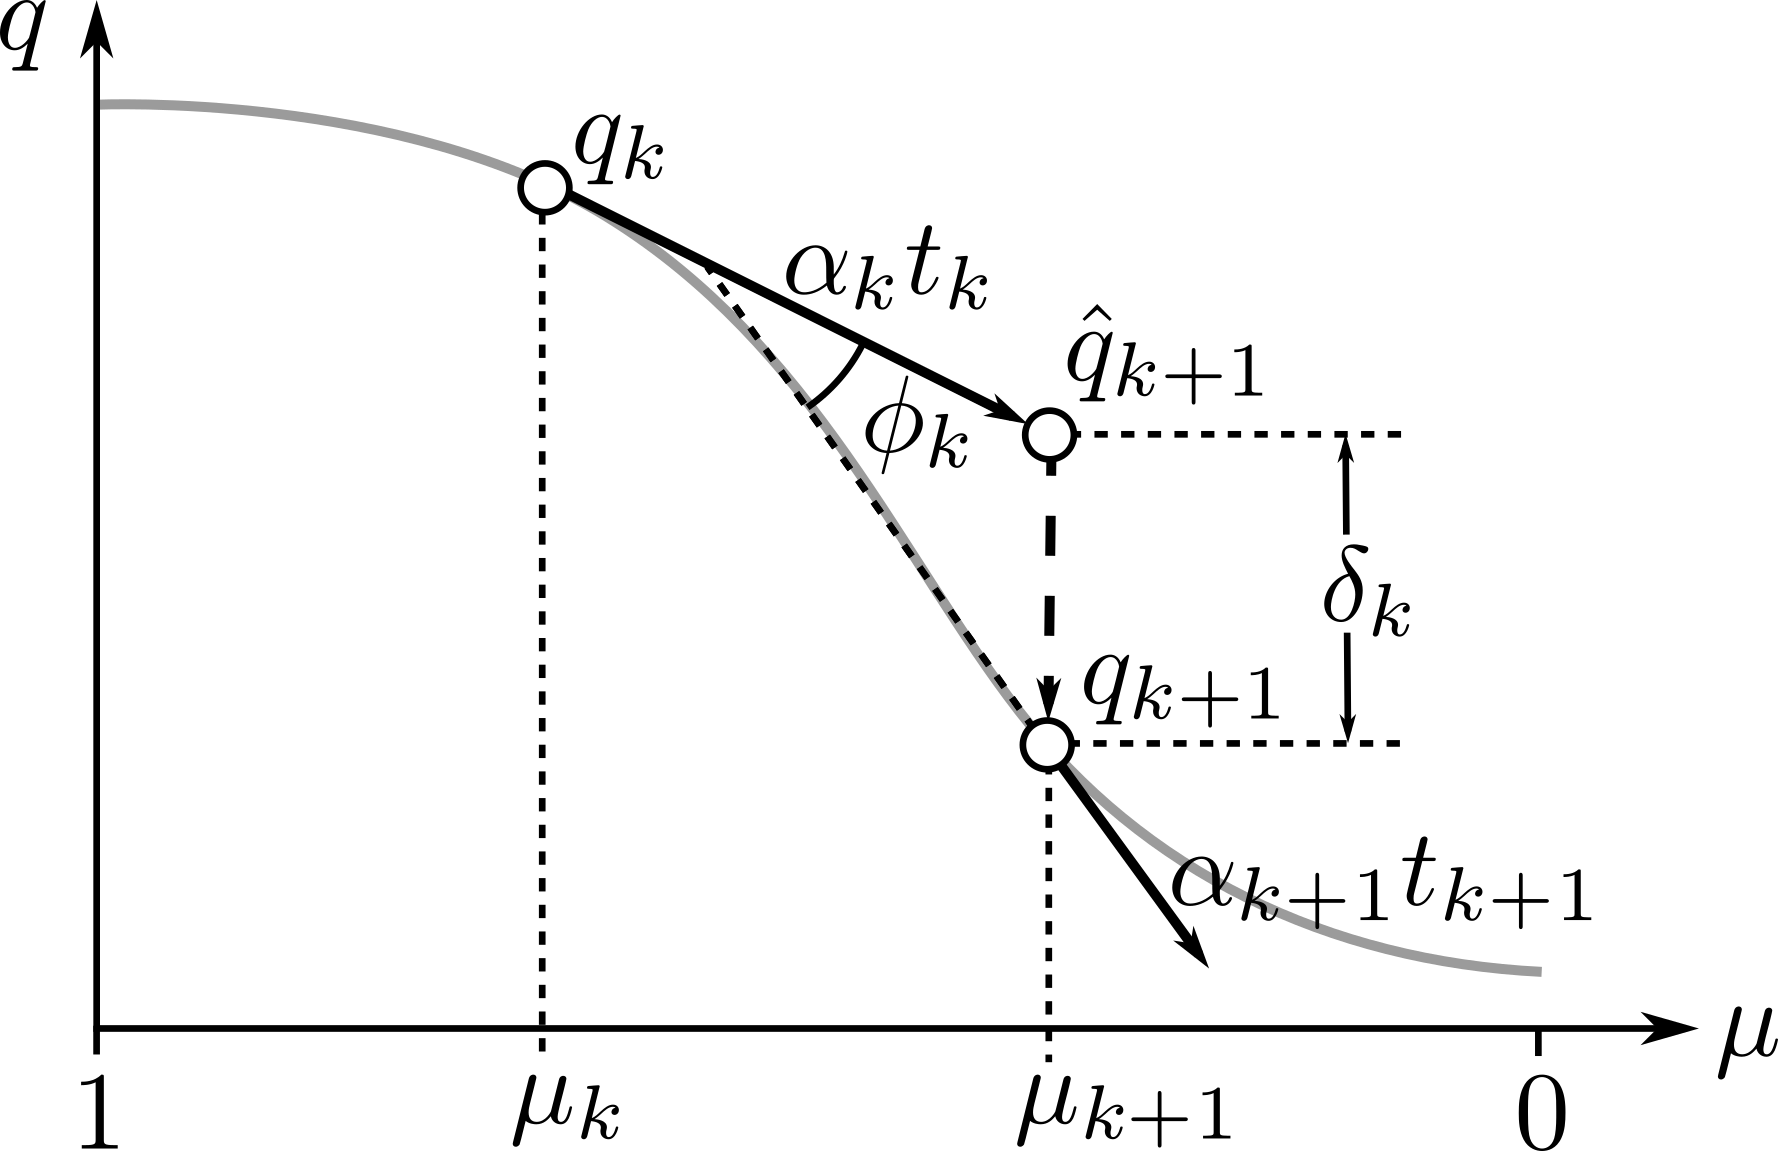
\includegraphics[width=0.4\linewidth]{figs/chap2/exact_pc.png} }
  \hspace{3em}
  \subfloat[inexact solves\label{fig:inexact_pc}]{
  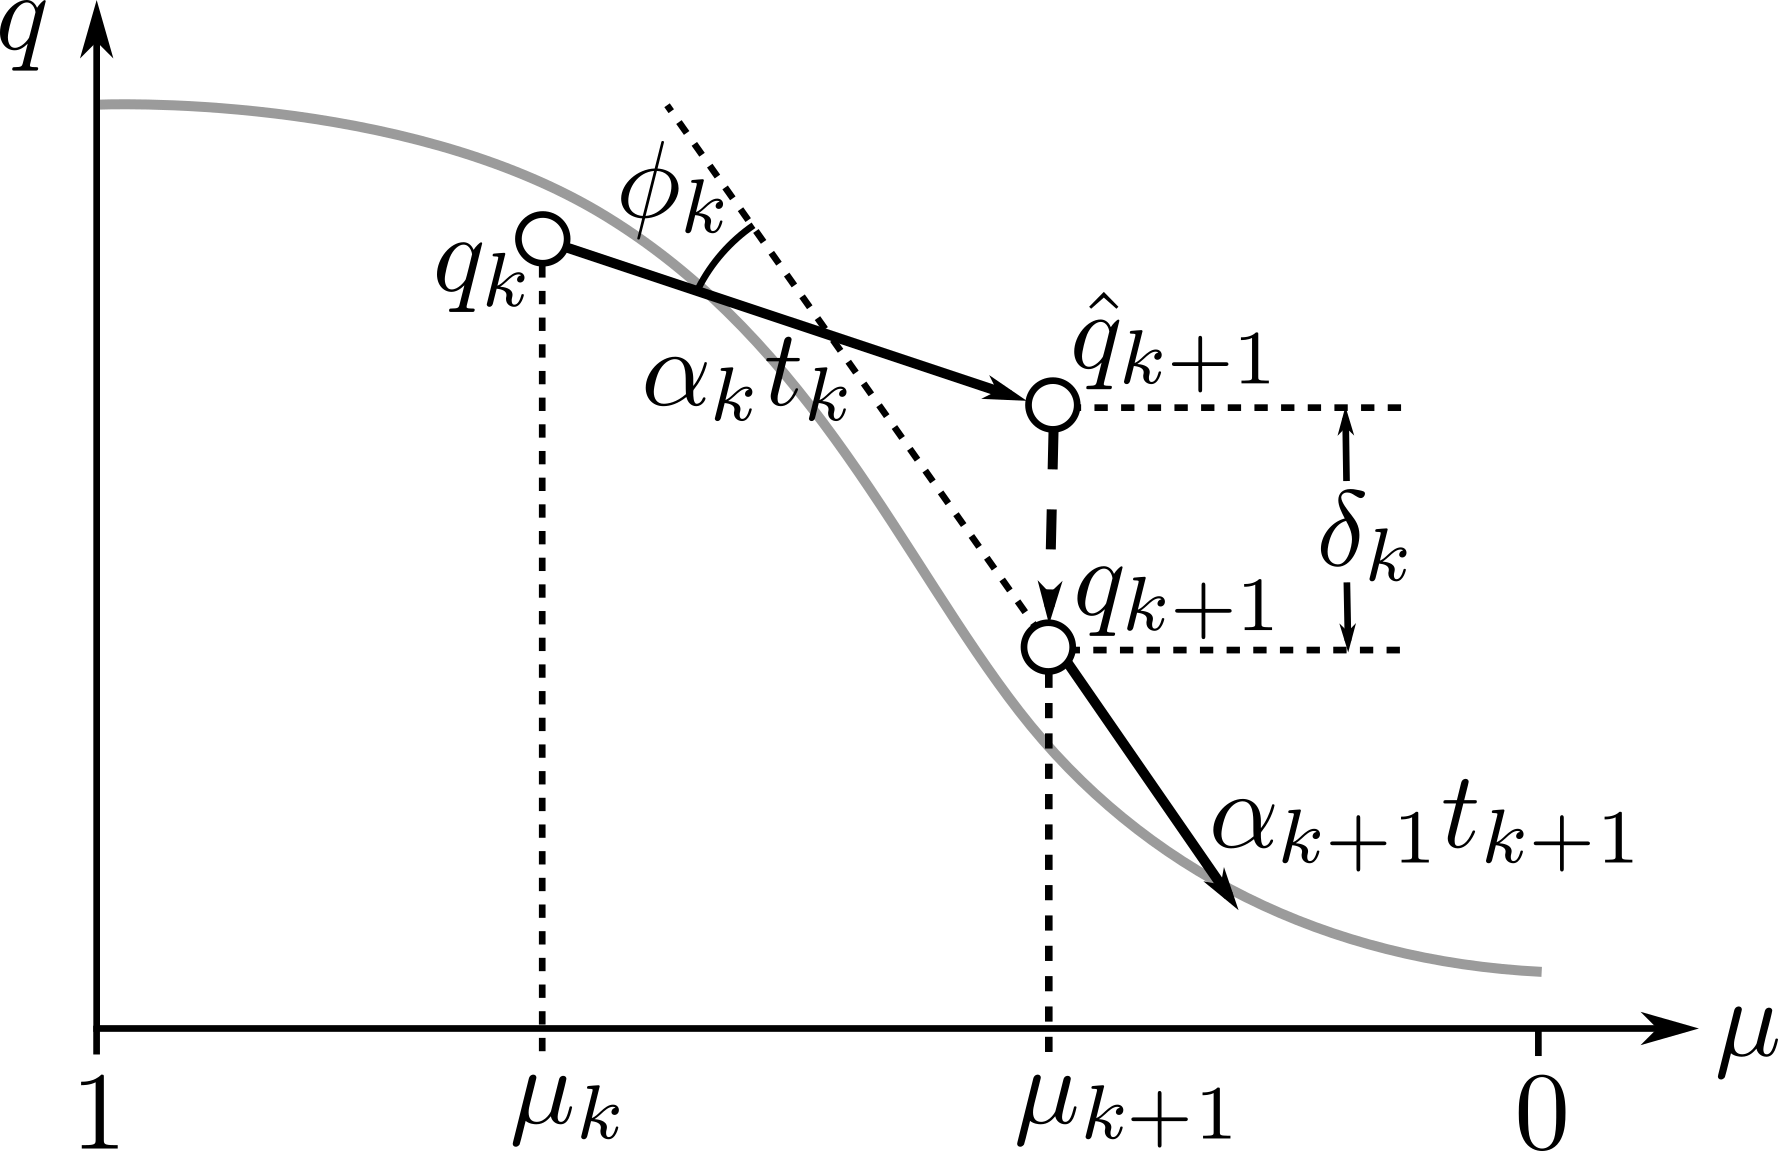
\includegraphics[width=0.4\linewidth]{figs/chap2/inexact_pc.png}
  }
 \caption{ Figure~\ref{fig:exact_pc} illustrates the predictor-corrector algorithm in the case that exact solves are used, while Figure~\ref{fig:inexact_pc} depicts the situation when inexact solves are used. \label{fig:pc}}   
\end{figure}


\begin{description}

  \item[Predictor:] During the predictor phase we first need to compute an
    approximate tangent direction $q' = dq/d\mu$, which is defined by taking the
    total derivative of $H(q,q_0,\mu) = 0$ with respect to $\mu$, \ie the
    implicit function theorem:
    \begin{equation}
      \left(\nabla_q H\right)_{k} q_{k}' = -\nabla_\mu H_{k} = F(q_k)  - G(q_k,q_0)
      \label{eq:predictorx}
    \end{equation}
    where $\nabla_q H$ and $\nabla_\mu H$ are evaluated at $q_k$, the previous
    homotopy iterate.  In practice, we solve \eqref{eq:predictorx} inexactly
    using a preconditioned Krylov iterative method.  That is, we find a $q_{k}'$
    that satisfies
    \begin{equation*}
      \lVert \left(\nabla_q H\right)_{k} q_{k}' - F(q) + G(q,q_0) \rVert
      \leq \tau \lVert F(q_k)  - G(q_k,q_0) \rVert,
    \end{equation*}
    where $\tau \in [0,1)$ is the desired relative tolerance.  Further details
      on the inexact solution of \eqref{eq:predictorx} are provided in
      Chapter~\ref{chap:linsys}.
    
    After (inexactly) solving \eqref{eq:predictorx} for $q_{k}'$, the predictor
    step is given by
    \begin{equation*}\label{eq:pred}
      \begin{bmatrix}
        \hat{q}_{k+1} \\ \mu_{k+1} 
      \end{bmatrix} 
      = \begin{bmatrix}
        q_k \\ \mu_k 
      \end{bmatrix}      
      + \alpha_{k} t_{k},
    \end{equation*}
    where $\alpha_{k}$ is the step length taken along the tangent direction at
    iteration $k$ (see Section~\ref{sec:step}), and $t_k$ is the normalized
    tangent given by
    \begin{equation*}
      t_{k} \equiv \frac{1}{\sqrt{\|q_{k}'\|^2 + 1}} \begin{bmatrix} -q_k'
        \\ -1 \end{bmatrix}.
    \end{equation*}
    Note that the negative signs in the definition of $t_k$ account for
    decreasing $\mu$ as the path moves from $\mu=1$ to $\mu <
\epsilon_\mu$.

  \item[Corrector:] In the corrector phase, we fix the homotopy parameter
    at $\mu=\mu_{k+1}$ based on the predictor, and use a Newton-Krylov method to
    inexactly solve $H(q_{k+1},q_0,\mu_{k+1}) = 0$.  This has the effect of
    ``correcting'' $\hat{q}_{k+1}$ to be closer to the path.  More precisely,
    we seek $q_{k+1}$ that reduces the relative residual below some tolerance:
    \begin{equation}\label{eq:cornt}
      \lVert H(q_{k+1},q_0,\mu_{k+1}) \rVert \leq
      \epsilon_k \lVert H(\hat{q}_{k+1},q_0,\mu_{k+1}) \rVert.
    \end{equation}
    A loose relative tolerance of $\epsilon_k \in [0.1,0.5]$ is used for
    homotopy parameter values $\mu > 0$ to avoid oversolving the corrector step.
    Once the algorithm reaches $\mu = 0$, the tolerance is tightened to the
    user-specified value for the first-order necessary conditions.
    
    At each Newton subiteration within the corrector, we must solve a linear
    system of the form
    \begin{equation}\label{eq:cor}
      \left(\nabla_q H \right)_{k+1} \Delta q_{k+1} = -H,
    \end{equation}
    for $\Delta q_{k+1}$, where $(\nabla_q H)_{k+1}$ and $H_{k+1}$ are evaluated
    at $\mu_{k+1}$ and the current estimate for $q_{k+1}$.  The Jacobian,
    $\nabla_q H$, that appears in \eqref{eq:cor} also appears in
    \eqref{eq:predictorx} during the predictor phase; again, further details
    regarding the solution of the linear systems that involve $\nabla_q H$ are
    provided in Chapter~\ref{chap:linsys}.

\end{description}

\begin{remark}
  The above predictor-corrector approach is a classical embedding
  method~\cite{allgower_georg_1993}, since the solution path is assumed to be
  parameterized by $\mu$; that is, the path has the form $(q(\mu),\mu)$.  This
  type of method cannot handle folds, or turning points, where the path reverses
  direction with respect to $\mu$ and the Jacobian $\nabla_q H$ becomes
  singular.  Problems for which such turning points arise can be handled using
  more advanced predictor-corrector algorithms; see, for
  example,~\cite{walker:1999}.
\end{remark}

\subsection{Implementation details}

\subsubsection{Adaptive step-size control}\label{sec:step}

The step length $\alpha$ along the tangent direction is calculated using the
asymptotic expansion method \cite{allgower3}, which we briefly review here.

At the first iteration of the predictor-corrector algorithm when $\mu=1$, a
conservative step length is used, \eg, $\alpha_0 = 0.05$.  Subsquent step
lengths are then determined adaptively using a scaling factor and a couple
safeguards on the maximum step size:
\begin{equation*}
  \alpha_{k} = \min\left( \sqrt{\|q_{k}'\|^2 + 1}\Delta \mu_{\max}, \alpha_{\max}, \alpha_{k-1}/\zeta_{k} \right),
\end{equation*}
where $\Delta \mu_{\max}$ is the maximum allowable change in $\mu$,
$\alpha_{\max}$ is allowable step size permitted by the fraction-to-the-boundary
rule (see Section~\ref{sec:fraction}), and the scaling factor is given by
\begin{equation*}
  \zeta_{k} \equiv \max\left( \sqrt{\delta_k/\delta_{\text{targ}}}, \phi_k / \phi_{\text{targ}} \right).
\end{equation*}

The scaling factor $\zeta_k$ is controlled by two quantities that measure how
nonlinear the path is, namely the previous corrector update size, and the angle
between successive tangents.  Referring to Figure~\ref{fig:pc}, the corrector
update size is the magnitude of the difference between the predictor step and
the corrector step:
\begin{equation}\label{eq:delta_k}
  \delta_k \equiv \| q_{k} - \hat{q}_{k} \|.
\end{equation}
A large value of $\delta_k$ indicates that the linear predictor does not
approximate the path well, so a smaller step size is warranted.  The angle
between the tangents is
\begin{equation}\label{eq:phi_k}
  \phi_k \equiv \arccos\left(t_{k+1}^T t_{k} \right).
\end{equation}
The angle $\phi_k$ is a measure of the curvature in the path, so a relatively
large value of $\phi_k$ also suggests that $\alpha_k$ should be reduced.  For
locally linear paths both $\delta_k$ and $\phi_k$ are zero, and the scaling
factor will lead to an unbounded $\alpha_k$; hence the need for the maximum
allowable step $\alpha_{\max}$.

\begin{remark}
  While the adaptive step-size control is automated, performance depends on the
  parameters $\alpha_0$, $\Delta \mu_{\max}$, $\delta_{\text{targ}}$ and
  $\phi_{\text{targ}}$.  The optimal choice for these parameters is problem
  dependent.
\end{remark}

\subsubsection{Safeguards on the slacks and inequality multipliers}\label{sec:fraction}
One of the differences between solving \eqref{eq:opt00x} and solving a generic
nonlinear system of equations is that the slacks and inequality multipliers must
remain nonnegative and nonpositive, respectively.  To cope with this additional
set of requirements, the following safeguards are implemented in the
predictor-corrector scheme.
\begin{itemize}
  \item During the predictor phase, the maximum allowable step size is bounded
    using a fraction-to-the-boundary-like rule~\cite{Nocedal2006NO} defined
    below.
    
  \begin{equation}\label{eq:f2b}
      \alpha_{\max} = \max\left\{
      \alpha \in (0,1] \;|\; s + \alpha s' \geq \tau_s .\right\}.
    \end{equation}
where $\tau_s = 10^{-6}$. If a particular slack variable gets close to zero, 
   \begin{equation*}
   0 <  s \leq \tau_s
   \end{equation*}
  then its value is frozen and it is excluded from the above
    calculation of $\alpha_{\max}$.

In our algorithm, we make sure the slack variables $s \geq \tau_s$ at the very beginning 
to the initial slack $s_0$ as well as at the last point of the corrector step 
by applying the following clipping rule : 
   \begin{equation}\label{eq:sclip}
      \hat{s} = \max(s, \tau_s)
   \end{equation}


    The maximum step size is enforced for all variables, including the design
    variables $x$.  We have found that synchronizing the step size across the
    design, slack and multipliers improves the performance of the algorithm.
    
  \item After the predictor step, and the corrector step,
  the inequality multipliers are clipped to
    ensure they remain non-positive:
    \begin{equation}\label{eq:lclip}
      \hat{\lambda}_{k+1} = \min(\lambda_{k} + \alpha_k (t_k)_{\lambda}, 0),
    \end{equation}
    where $(t_k)_{\lambda}$ denotes the multiplier component of the normalized
    tangent, and the $\min$ function in the above expression is to be
    interpreted elementwise.
    
\end{itemize}

While the slacks and multipliers both have bound constraints, their treatment is
slightly different in the above safeguards.  Our motivation for bounding the
slacks away from zero, in both the predictor corrector phases, is to avoid
severe ill-conditioning in the system matrix and its preconditioner; see
Section~\ref{sec:matfreepc} for further details.  The multipliers, in contrast,
do not lead to conditioning problems if they vanish, so we can clip the
multipliers to zero.

\subsection{Algorithm Summary}

With most of its elements described, we summarize the predictor-corrector method
in Algorithm~\ref{alg:pc}.  The solution of the tangent step,
line~\ref{line:tang}, and the solution of the Newton step, line
\ref{line:newton}, are the only components of the algorithm that require further
explanation.  % The solution of these linear systems is detailed in the next chapter.
\\
\LinesNumberedHidden
\begin{algorithm}[H]\setstretch{1.35}
\SetKwInOut{Input}{Input}
\SetKwInOut{Output}{Output}
\SetKwInOut{Parameter}{Parameters}
\SetKw{Break}{break}
\SetKw{Return}{return}
\SetEndCharOfAlgoLine{}
%\SetKwRepeat{Do}{do}{while} %

\Parameter{$K_{\max}$, $J_{\max}$, $\epsilon_F$, $\tau$, $\epsilon_H$, $\alpha_0$, $\delta_{\text{targ}}$, $\phi_{\text{targ}}$, $\Delta \mu_{\max}$}
\Input{$x_0$, $s_0$}
\Output{$q^{*} = \begin{bmatrix} x^{*T} & s^{*T} & \lambda_h^{*T} & \lambda_g^{*T}   \end{bmatrix}^T$, the solution of \eqref{eq:opt00x}}
\BlankLine
Clip $s_0$ if necessary: $s_0 \leftarrow \max(s_0,\tau_s)$  \\
Set $q_0 = \begin{bmatrix} x_0^T & s_0^T& 0^T & 0^T \end{bmatrix}$, $q  \leftarrow q_0 $  \\
compute state $u$,  adjoint $\psi$ for $\boldsymbol{q}_0$ \\
inexactly solve $\left(\nabla_q H\right)_{k} q_{k}' = - \nabla_\mu H_{k}$ 
 for $q_{k}'$ to required tolerance $\tau$ \label{line:initPred} \\
compute the normalized tangent direction $t_{k}$ using \eqref{eq:tk} \\

\For{$k = 0,1,2,\ldots,K_{\max}$}{
 compute $\alpha_{k} (\alpha_0 \text{~if~} k==0) = \min\left( \sqrt{\|q_{k}'\|^2 + 1}\Delta \mu_{\max}, \alpha_{\max}, \alpha_{k-1}/\zeta_{k} \right)$\\
  use \eqref{eq:pred} to update $\hat{q}_{k+1}$ and $\mu_{k+1}$\\
  clip $\lambda_{k+1}$ if necessary:  $\hat{\lambda}_{k+1} = \min(\lambda_{k} + \alpha_k (t_k)_{\lambda}, 0)$  \\
  update state $u$, adjoint $\psi$ at $\boldsymbol{q}_{k+1}'$ \\
  set $q_{k+1} \leftarrow \hat{q}_{k+1}$\\
  
  \For{$j = 0,1,2,\ldots,J_{\max}$}{ 
    \lIf{$\lVert H(q_{k+1},q_0,\mu_{k+1}) \rVert \leq \epsilon_{H} \lVert
      H(\hat{q}_{k+1},q_0,\mu_{k+1}) \rVert$}{%
      \Break
    }
    \ShowLn
    inexactly solve $\left(\nabla_q H \right)_{k+1} \Delta q_{k+1} =
    -H_{k+1}$ for $\Delta q_{k+1}$ \label{line:newton} \\
    $q_{k+1} \leftarrow q_{k+1} + \Delta q_{k+1}$ \\
     \lIf{ $\mu_{k+1} < \epsilon_{\mu}$ and $\| F(q_{k}) \| \leq \epsilon_{F} \|F(q_{0})\|$,  $s_{i} \geq 0$}
     {\Break \Break} 
  }
  update state $u$, adjoint $\psi$ at $\boldsymbol{q}_{k+1}$ \\ 
    \lIf{$\| F(q_{k}) \| \leq \epsilon_{F} \|F(q_{0})\|$,  $s_{i} \geq 0$ ,
   and $\lambda_{i} \leq 0$}{\Return $q_{k}$}
  \ShowLn
   inexactly solve $\left(\nabla_q H\right)_{k} q_{k}' = - \nabla_\mu H_{k}$
  for $q_{k}'$ to required tolerance $\tau$   \label{line:tang} \\
  compute the normalized tangent direction $t_{k}$ using \eqref{eq:tk} \\
  compute the step scaling factor: $\zeta_{k} = \max\left( \sqrt{\delta_k/\delta_{\text{targ}}}, \phi_k / \phi_{\text{targ}} \right)$\\
  compute $\alpha_{k} = \min\left( \sqrt{\|q_{k}'\|^2 + 1}\Delta \mu_{\max}, \alpha_{\max}, \alpha_{k-1}/\zeta_{k} \right)$\\
  clip $\lambda_{k+1}$ and $s_{k+1}$ if necessary: $s_{k+1} \leftarrow \max(s_{k+1},\tau_s)$ and
  $\lambda_{k+1} \leftarrow \min(\lambda_{k+1},0)$ \\
  update $\delta_k$ and $\phi_{k}$ according to \eqref{eq:delta_k} and
  \eqref{eq:phi_k} \\
  $k \leftarrow k+1$
  }
\caption{Inexact-Newton predictor-corrector algorithm for PDE-Constrained
  optimization.\label{alg:pc}}
\end{algorithm}

\newpage
%%%%%%%%%%%%%%%%%%%%%%%%%%%%%%
\section{Application I: Sphere Problem}
\subsection{Problem Description}
The first test problem to verify RSNK's globalization performance is on an analytical inequality constrained Sphere problem: 
\begin{equation*}
\begin{aligned}
\underset{x, y, z} {\text{min}}  & \quad & x + y + z \\
   {\text{subject to}}  & \quad & x^2 + y^2 + z^2 <= 3 \\
\end{aligned}
\end{equation*}

The solution to this problem is at $(-1,-1,-1)^T$. There is a local maximum point at $(1,1,1)^T$, where the 
first-order optimality condition (KKT condition) is also satisfied but not the second-order optimality condition. 

\subsection{Results}
To prove that the algorithm can bypass the local maximum, 100 random starting points around $(1,1,1)^T$ are generated using Gaussian random distribution, with a mean at 1, and standard deviation 0.1. Figure~\ref{fig:sphere_100} shows the sphere, with the starting points in blue circles, and the solutions in red starts. 

 \begin{figure}[H]
  \centering
  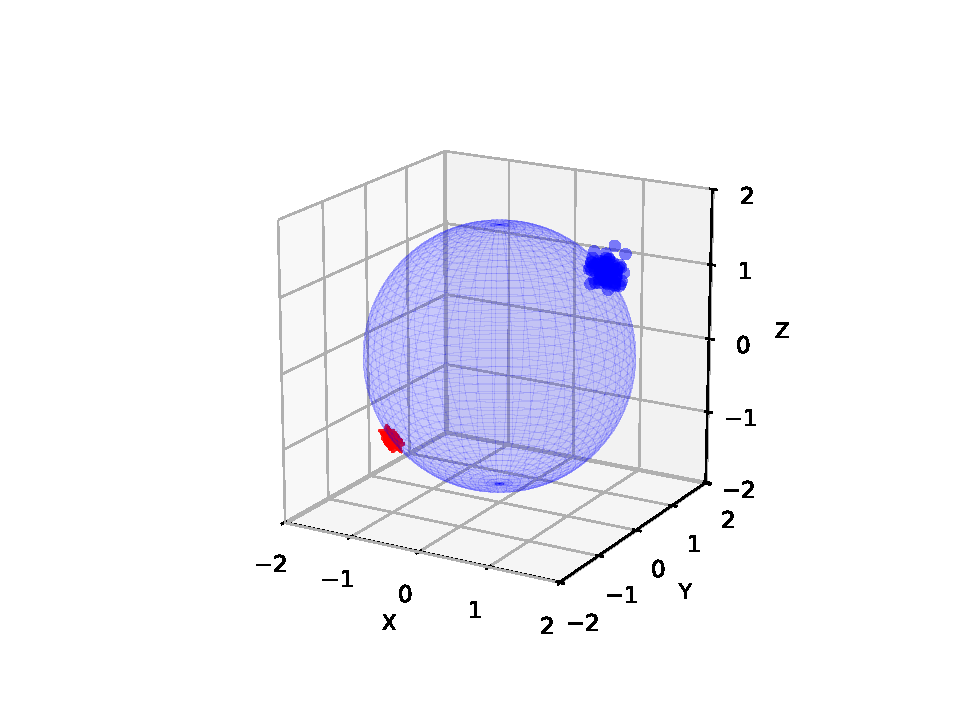
\includegraphics[clip,trim=20 40 20 70, width=1.0\columnwidth]{./figs/chap2/100_111.pdf}%  
  \caption{100 Starting Points Around Local Maximum \label{fig:sphere_100}}
\end{figure}


 \begin{figure}[H]
  \centering
  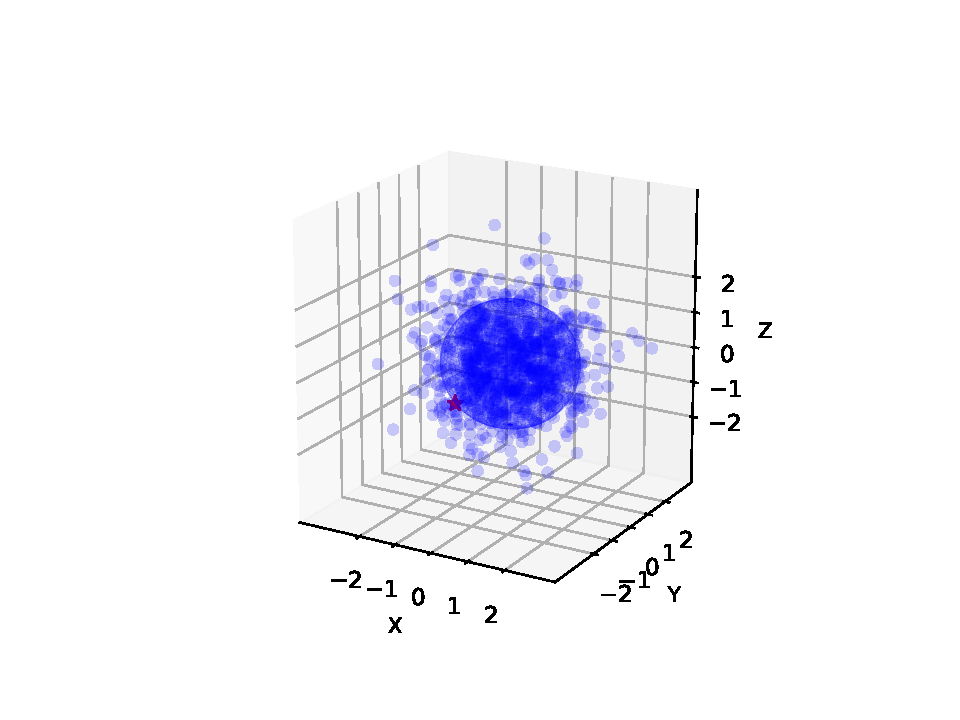
\includegraphics[clip,trim=80 40 20 70, width=1.1\columnwidth]{./figs/chap2/1000.pdf}%  
  \caption{1000 Random Standard Distributed Points \label{fig:sphere_1000}}
\end{figure}

 \begin{figure}[H]
  \centering
  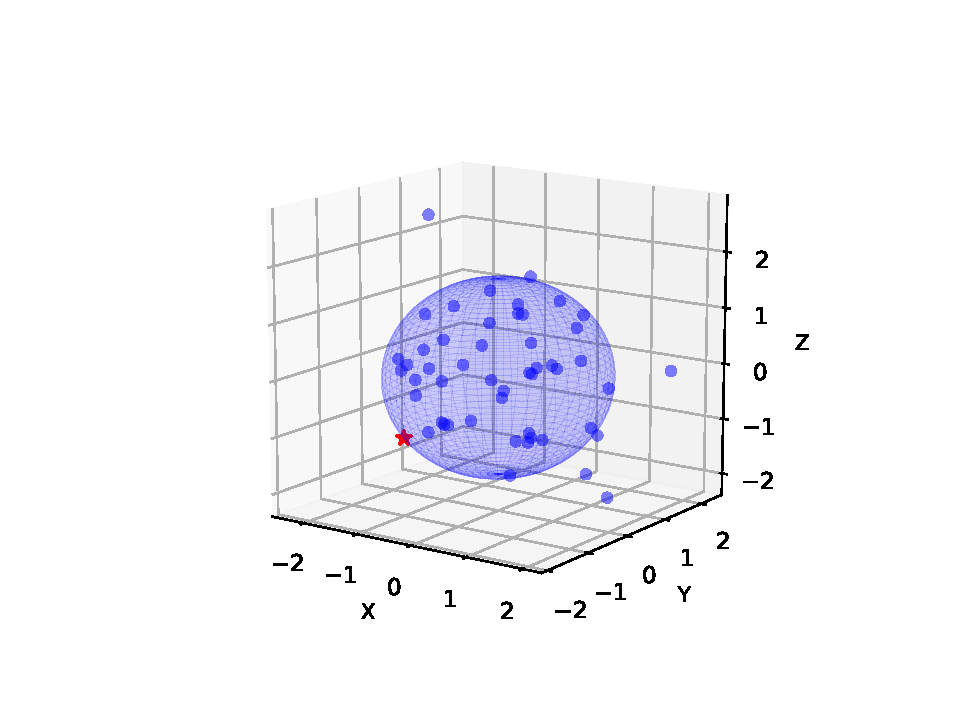
\includegraphics[clip,trim=50 50 20 75, width=1.0\columnwidth]{./figs/chap2/50.pdf}%  
  \caption{50 Random Standard Distributed Points \label{fig:sphere_50}}
\end{figure}

Figure~\ref{fig:sphere_1000} shows the distribution of 1000 starting points generated using the Standard 
Normal Distribution method. The starting points are semi-transparent blue circles, while the solution points are in solid red stars. The red star shown in the picture is actually 1000 solutions points overlaid on top of each other. 
Figure~\ref{fig:sphere_50} shows the same content but with 50 starting points. The test shows that the globalization of RSNK is working well.  


%%%%%%%%%%%%%%%%%%%%%%%%%%%%%%
\section{Application II: Non-convex Problem}
\subsection{Problem Description}
We consider the following simple nonconvex optimization problem :
\begin{equation*}
\begin{aligned}
&\underset{x \in R^{100}} {\text{min}}  
& &\phantom{-} \frac{1}{2}x^T \mat{Q} x \\
  & {\text{subject to}}
& &-1 \leq x_i \leq 1 \qquad \forall i = 1,2,\ldots,100 \\
\end{aligned}
\end{equation*}
where the pattern of $\mat{Q} = \textsf{diag}(1,-1,1,\ldots,1,-1)$ is randomly generated. 

This problem is challenging for Newton-based optimization algorithms, which 
tends to locate stationery points where $F(q) = 0$ but cannot differentiate between 
a minimizer or a maximizer. As the objective function can be separated into 
individual dimensions, it is easy to see that the minimizer for this problem has the pattern
corresponding to $\mat{Q}$: 
\begin{equation}\label{eq:pattern}
  x^{*} = \begin{bmatrix} 0 & \pm 1 & 0 & \cdots & 0 & \pm 1 \end{bmatrix}^{T}.
\end{equation}
where
\begin{equation}\label{eq:pattern2}
  \begin{gathered}
  x_i=0  \text{~if~}  \mat{Q}_{ii} = 1  \\
  x_i = \pm 1  \text{~if~}  \mat{Q}_{ii} = -1
  \end{gathered}
\end{equation}
We would like to see 
the ability of the algorithm to bypass the wrong solutions in individual dimensions, e.g. $x_i = 0$ 
when $\mat{Q}_{ii} = -1$ and $x_i = \pm 1$ when $\mat{Q}_{ii} = 1$.
Note that when $\mat{Q}_{ii} = 1$, the upper and lower bound $x_i = \pm 1$ are 
individual maximums where the gradient of the Lagrangian is zero in that dimension. 

\subsection{Results - Nonconvexity}
We ran the optimization algorithm on 1000 random cases. For each case, 
the arrangement of $1$ and $-1$ in $\mat{Q}$ is uniformly randomly generated; 
 the initial point $x_0$ is also generated randomly with uniform probability in the domain
  $\Omega = \{ x \in \mathbb{R}^{100} \; | \; -2 \leq x_i \leq 2 \}$.  We call a solution successful if 
  its pattern is exact as \eqref{eq:pattern2}.  Table~\ref{tab:success} lists the success rate for different 
  combinations of $\epsilon_{\text{krylov}}$ and $\epsilon_F$. 
 
\begin{table}[H]
  \begin{center}
    \caption{Success Rate with Different Parameters \label{tab:success}}
  \begin{tabular}{| c |  c |  c |  c | c | c | c | c |}
  \hline
 & \multicolumn{7}{  c  | }{ $\epsilon_{\text{krylov}}$  } \\  \hline
 &   & 1e-1  & 1e-2    & 1e-3    &  1e-4    &  1e-5   & 1e-6  \\  
\multirow{2}{*}{$\tau$ and $\epsilon_F$ } &  1e-1 & 51\%  &90.0\% &94.2\% &94.6\% &93.9\% & 93.8\%  \\
	               					      &   1e-2 & 47.2\%  &93.1\% &94.4\% &93.9\% &94.2\% &  94.5\%\\
    \hline
  \end{tabular}
  \end{center}
\end{table}

As can be seen from Table~\ref{tab:success}, the robustness of the algorithm for handling non-convexity 
is obviously impacted by the tolerances. It shows that $\epsilon_{\text{krylov}}$ has to be below $1e-2$ 
for effective non-convexity handling ability, and the predictor and corrector linear solve tolerance $\epsilon_F$ 
plays a smaller role than $\epsilon_{\text{krylov}}$.   
  
 \begin{figure}[tbp]
  \centering
  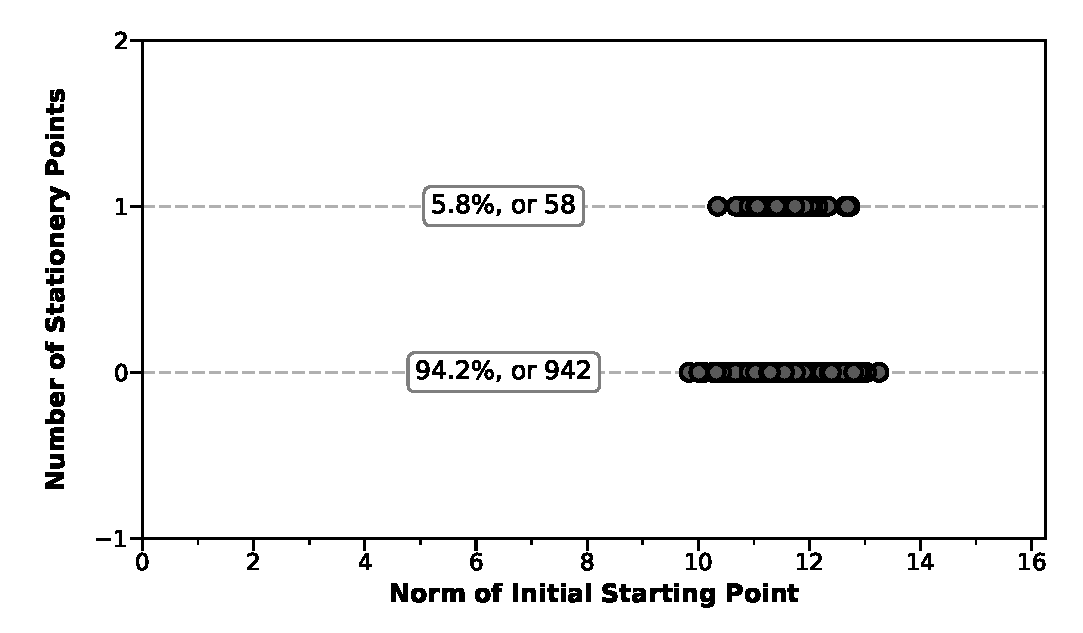
\includegraphics[clip,width=0.7\columnwidth]{./figs/chap4_test/nonconvex_1000_random.eps}%
  \caption{Success Minimizers. \label{fig:nonconvex}}
\end{figure}

Figure ~\ref{fig:nonconvex} shows one sample statistical results for the random study using 
$\epsilon_{\text{krylov}}=10^{-5}$ and $\tau = 10^{-2}$. The plot shows that $94.2\%$ of the $1000$ random cases 
successfully converge to the minimizer, while the rest $5.8\%$ of the $1000$ cases failed in one dimension.    
  
The results show that the optimization method can start from infeasible points, and can handle certain 
amount of nonconvexity. The preconditioner is not used here.  Admittedly, this nonconvex test problem is rather simple, with no complexities like bad-scaling, ill-conditioning included. However, the focus is solely to see whether the added regularization from the homotopy term can help 
Newton's method bypass local maximization points.  Further work is needed to determine when the problem demands 
tighter tolerances and how to detect and handle nonnegative curvature.  

 \subsection{Results - Convergence Plots} 
 
A typical optimization convergence plot is provided in Figure~\ref{fig:nc_converg}. Figure~\ref{fig:ncmu} 
shows the absolute optimality, complementarity and feasibility at each Homotopy iteration of different $\mu$. 
Note that for simplicity, only the Predictor points are displayed when $\mu \geq \epsilon_{\mu}$, 
while the Corrector points are displayed at $\mu < \epsilon_{\mu}$.
Figure~\ref{fig:nccpu} shows convergence plot w.r.t CPU time, 
which is used more often later when the performance of the new method is benchmarked with other 
optimization packages.

\begin{figure}[tbp]
  \centering
  \subfloat[Convergence vs. $\mu$ \label{fig:ncmu}]{
   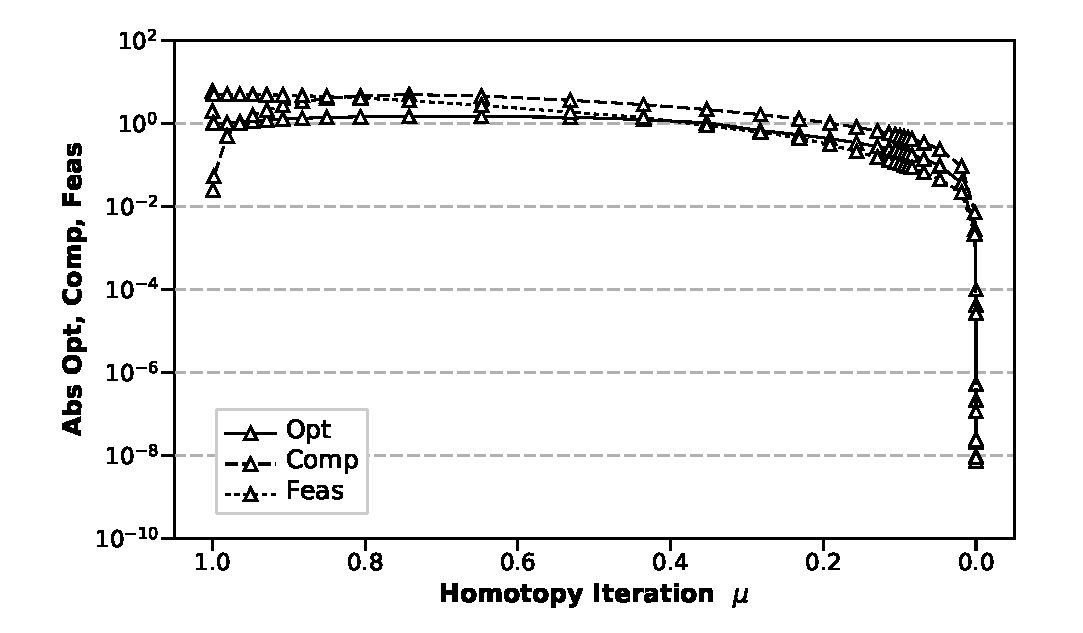
\includegraphics[clip,width=0.7\linewidth]{./figs/chap4_test/nonconvex_mu.eps} }
   \hspace{1em}
   \subfloat[Convergence vs. CPU time \label{fig:nccpu}]{
   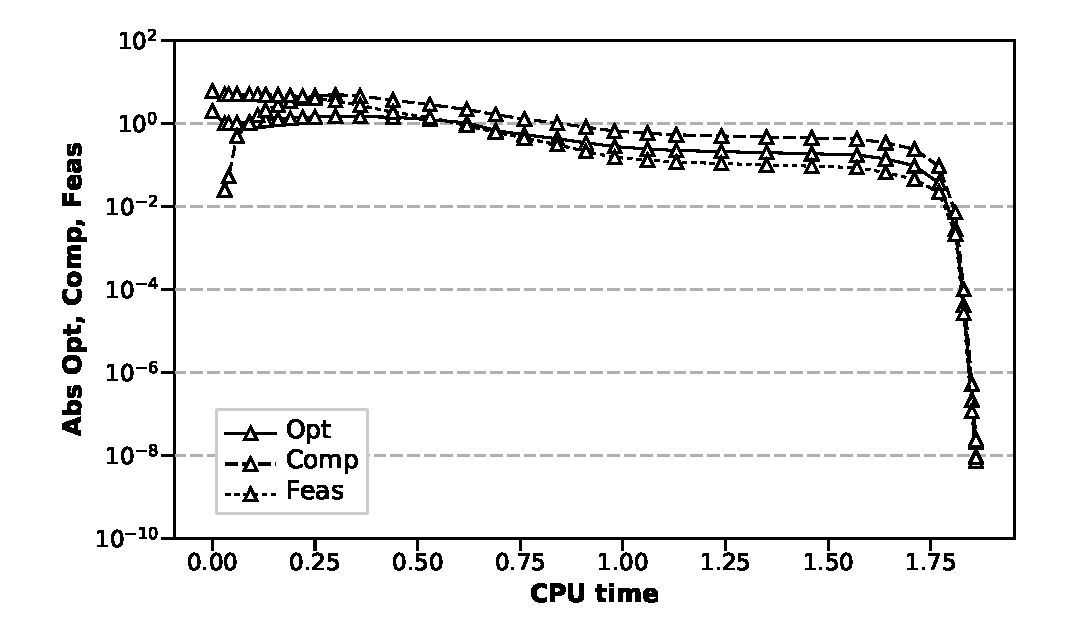
\includegraphics[clip,width=0.7\linewidth]{./figs/chap4_test/nonconvex_cpu.eps} }
   \caption{Typical Convergence Plots in $1000$ Random Cases \label{fig:nc_converg}}
\end{figure}

%\begin{remark}
% The parameters $\alpha_0$, $\delta_{\text{targ}}$, $\phi_{\text{targ}}$, and
%  $\Delta \mu_{\max}$ all play a role in the ability of Algorithm~\ref{alg:pc}
%  to handle nonconvex objectives.  If these parameters are set too agressively,
%  then the algorithm may move off the homotopy level-set and converge to a local
%  maximizer or saddle, even for the simple problem considered here.
%  \padd{I think this Remark should be removed now. As we've provided the influence of 
%  Krylov tolerance and inner tolerance on the success rate. }
%\end{remark}



%%%%%%%%%%%%%%%%%%%%%%%%%%%%%%%%%%%%%%%%%%%%%%%%%%%%%%%%%%%%%%%%%%% 
%                                                                 %
%                            CHAPTER FOUR                        %
%                                                                 %
%%%%%%%%%%%%%%%%%%%%%%%%%%%%%%%%%%%%%%%%%%%%%%%%%%%%%%%%%%%%%%%%%%% 
 
\chapter{CUTER TEST PROBLEMS}

In this chapter, we test the Homotopy RSNK optimization algorithm and the preconditioners 
on two constructed analytical problems to investigate the algorithm's non-convexity 
handling capacity and scalability performance. The first one is a constructed indefinite 
quadratic problem with bound constraints. The second one is a constructed convex 
quadratic problem with linear inequality constraints. The second problem is scalable with 
the problem dimension ranges from 100 to 500. A state-of-the-art optimization package 
SNOPT is benchmarked with on accuracy and scalability performance.   

\section{General Information for Test Problems}
\subsection{Optimization Environment - Kona}\label{sec:kona_mv}
The previously introduced Homotopy RSNK method and the preconditioners are part of 
our in-house optimization package, Kona~\cite{dener:scitech2016}. Kona is a matrix-free, 
parallel agnostic optimization package aiming for solving large-scale PDE-constrained 
optimization problems.  It has implemented several optimization 
algorithms including an unconstrained 
reduced-space quasi-Newton method, an unconstrained reduced-space 
Newton-CG method, an equality constrained reduced-space Newton-Krylov 
based on FLECS~\cite{hicken:flecs2014}, and a composite-step RSNK.    
It contains various types of tools for supporting the functions of the optimization algorithms, e.g. 
iterative matrix-free solvers like FGMRES, STCG, FLECS for the linear systems, 
globalization techniques including trust-region, backtracking line search and line search with 
the strong Wolfe conditions, and merit functions like augmented Lagrangian and $l_2$ 
merit function. Besides, it computes the matrix-vector product of the Hessian of the Lagrangian 
by solving two second-order adjoint systems. 

Architechturally, it separates the optimization algorithms with the optimization 
problem interface, allowing the development of new optimization algorithms independently with 
new problem solvers. From a user's perspective, one has to write a solver interface to Kona providing 
a series of function operations as listed in Table 4.1 in~\cite{dener_thesis_2017}. The solver interface 
functions the same as the objective/constraint function and the sensitivity function in SNOPT, or 
other popular optimization methods like fmincon in Matlab. During the optimization process, 
conventional optimizers will call those functions for evaluating the function values and sensitivities 
values at different design points, then make decisions on where to go for the next point. 
The sensitivities demanded are the total gradients. In presence of state variables for 
PDE-constrained optimization, total gradients are expensive as each one would require an adjoint solve, 
as explained in detail in Chapter~\ref{sec:pde_mot}. In contrast, the structure of the solver interface 
required by Kona is designed specially for PDE-constrained optimization problems by providing 
partial gradients instead of total gradients, and matrix-vector products with the system matrix of 
the PDE solvers, with the Jacobians of the constraints w.r.t. the state variables, and with 
the Jacobians of the constraints w.r.t. the design variables. These matrix-vector products 
with the Jacobians are used to assemble the matrix-vector products with the Lagrangian Hessian 
and the total constraint gradients, which in turn are used by the Krylov solvers to solve the linear systems.    

The Homotopy RSNK method developed in this work is placed together with the other unconstrained 
and equality constrained optimization methods, with the same interface and using the same 
vector and matrix operator modules. The preconditioners are likewise placed in the preconditioned folders. 
When testing different problems, the user will first write the solver interface, then setup the running script 
to execute the optimization. 

Although Homotopy RSNK's strength is in PDE-constrained optimization area in presence of 
state variables, it can still be used on problems without state variables, where the conventional 
optimization methods dominate.  For such problems, the total gradients are usually cheap to 
calculate and readily available. For instance, to solve a linear system involving the total constraint Jacobian, 
conventional optimization methods would ask to compute and 
store these total gradients for once, then find the solution by operating directly to the matrix entries.  
In contrast, when using the Homotopy RSNK method, it would ask to calculate the matrix-vector 
products several times in order to form the Krylov subspace. Each time the constraint Jacobian is 
calculated and multiplied with the incoming vector, then released from the memory space. 
So it's the memory cost of the storage of the matrix versus the computational cost of matrix-vector products 
for several times. For some problems, the matrix exists in the form of basic algebraic operations, saving the memory cost of storing the matrix even for once. 


\subsection{SNOPT}
SNOPT is short for Sparse Nonlinear OPTimizer~\cite{gill:2002}, a gradient-based sequential 
quadratic optimization method for solving large-scale nonlinear optimization problem 
with thousands of constraints and design variables. It uses an augmented Lagrangian 
merit function, and the Hessian of the Lagrangian is approximated
using a limited-memory quasi-Newton method. In this work, we use its Python interface 
pyOpt to compare its performance with that of the proposed Homotopy RSNK method. 
SNOPT uses major feasibility and major optimality to measure the progress of the 
optimization iteration. The feasibility measures the maximum nonlinear constraint violation, 
normalized by the size of the solution,
\begin{equation*}
\text{snopt feasibility} = \underset{i}{\text{max}}  \ \text{viol}_i / \lVert x \rVert 
\end{equation*}
where $\text{viol}_i$ is the violation of the $i$th nonlinear constraint~\cite{snopt_manual}. The feasibility tolerance 
$\epsilon_r$ is predefined, with a default value of $10^{-6}$. If it is known that some of the problem 
functions are of low accuracy, a larger value for the feasibility tolerance is appropriate. 

The optimality measures the maximum complementarity slackness for the design variables, 
and is calculated using the following formulas, 
\begin{equation*}
\text{snopt optimality} = \underset{j}{\text{max}}  \ \text{Comp}_j / \lVert \pi \rVert 
\end{equation*}
where $\text{Comp}_j$ measures the complementarity slackness for $j$th variable and is defined by:
\begin{equation*}
\text{Comp}_j = \begin{cases}
d_j \text{min} (x_j - l_j, 1)  \quad \text{if} \ d_j \geq 0 \\
-d_j \text{min} (u_j - x_j, 1) \quad \text{if} \ d_j < 0
\end{cases}
\end{equation*}
where $d_j = g_j - \pi^T a_j$ is the gradient of the Lagrangian, $g_j$ is the $j$th objective gradient, 
$a_j$ is the $j$th constraint Jacobian, $\pi$ is the dual variables. 

\subsection{Basic Settings for the Algorithm}
To measure the progress of the optimization iterations, we evaluate the infinite
norm of each row block in $F(x)$. Specifically, we will refer to optimality,
complementarity, and feasibility as defined below:
\begin{align*}\label{eq:optfeas}
\text{Optimality} &= \lVert   \nabla_x f(x) + \lambda^T \nabla_x g(x)  \rVert _{\infty} \\
\text{Complementarity} &=  \lVert   -\mat{S}\mat{\Lambda} e   \rVert _{\infty}   \\
\text{Feasibility} &= \begin{Vmatrix} h(x) \\ g(x) - s  \end{Vmatrix} _{\infty} 
\end{align*}

In the following tests, the convergence plots display the above metrics versus
computational cost.  Note that the absolute values of the above metrics are used, 
as the initial complementarity products are zero because of zero initial multipliers, 
and the initial feasibility is zero when we use $s_0 = g(x_0)$ for the inequality-only 
structural problem. 

For simplicity, the convergence plots show only the
predictor points before $\mu$ reaches $\epsilon_\mu$, plus all the corrector
points at the last homotopy iteration when $\mu < \epsilon_{\mu}$.

Table \ref{tab:param} shows the parameters used in the test problems, including
the default values set in the algorithm and the recommended ranges.

\begin{table}[tbp]
  \begin{center}
    \caption{Parameters used in the test problems \label{tab:param}}
  \begin{tabular}{ l c c c c c}
    \textbf{Parameters} & $\textbf{Default}$  & $\textbf{Range}$ & $\textbf{Nonconvex}$ 
    & $ \textbf{Quadratic} $ & \textbf{Structural}  \\ \hline
    %\rule{0ex}{3ex}%
    \multicolumn{6}{ l }{Predictor-Corrector Algorithm} \\   %  $\delta_{\text{targ}}$ and $\phi_{\text{targ}}$. 
    \hline
    $K_{\max}$             	&  100     & $\geq$100         & 100 	 &  100       &    100     \\ 
     $J_{\max}$  		&   2         & $\geq$2         & 2             & 2           &      2        \\
    $\epsilon_F$ 	           		&  1e-6     & [1e-8, 1e-3]   & 1e-7 	 & 1e-7       &    1e-4    \\ 
       $\tau$    		&   0.1      & [0.1,0.5]	        & 0.1          & 0.1	 &     0.1    \\
    $\epsilon_H$    		&   0.1      & [0.1,0.5]	        & 0.1          & 0.1	 &     0.1    \\
    $\epsilon_{\mu} $   & 1e-9     & [1e-10, 1e-6]  &   1e-9  & 1e-9  & 1e-6  \\   
    \textbf{$\alpha_0$}             &  0.05     & $\geq$0.01         & 0.05	 & [40,60,80,100,120]  &  0.05  \\
    $\delta_{\text{targ}}$      &  1.0	& [1.0,10]          & 10		 & 10    &   1.0    \\
    $\phi^{\circ}_{\text{targ}}$   & 10.0	& [5.0,50] 	       & 10		 & 20    &   10     \\
    $\zeta_{\max}$ 		        &  50		& [10,50]	       & 50		 & 50    	 &   50     \\
    $\zeta_{\min}$ 		        &  0.5	& 0.5		       & 0.001	 & 0.001    &   0.5   \\
    $\Delta \mu_{\max}$		        &  -5e-4	& [-5e-4, -5e-1]  & -5e-4	 & -5e-4     &  -5e-4  \\  
    $\Delta \mu_{\min}$		        &  -0.9	& -0.9 	       & -0.9		 & -0.9       &  -0.9    \\
    $s_0$                           & $\mathbf{e}$     &   $>$ 0    &    5$\mathbf{e}$    &  10$\mathbf{e}$   &  $g(x_0)$  \\ 
    $\tau_s$                      & 1e-6    & 1e-6    &  1e-6    &  1e-6    & 1e-6   \\
    \hline
    \multicolumn{6}{ l }{Preconditioner} \\ 
    \hline    
    $\mathbf{{n_{\mat{\Sigma}}}}$    & 5	       & $\geq$2		&  -	         &  2          &  [20,80,320]  \\
    $\beta$				& 1.0	       & $>$0        & -         &  -      &  0.1  \\
    $N_{\text{bfgs}}$		& 10	       & [1, 20]		& - 		 &  10	& -  \\
    $\mu_e$			& -1	       & [0, 1] 		& -	         &  -	        & 1e-3  \\
    $\Sigma_e$			& 1 	       & [0, 1]                 & -		& -		& 1e-3  \\
    \hline
    \multicolumn{6}{ l }{Krylov Iterative Solver} \\ 
    \hline       
    $n_k$		& 20        & [10,30]              & 20		 &  20       &  20  \\
    $\epsilon_{\text{krylov}}$		& 1e-2     & [0, 0.1]           	&1e-2	 &  1e-2    &  1e-4  \\
    \hline
  \end{tabular}
  \end{center}
\end{table}

\section{CUTEr Problem Description}\label{sec:cuter1}
The \textbf{CUTEr} Test Problem Set~\cite{cuter_opt, cuter_gould} is a huge collection of test problems to test new optimization codes and develop new algorithms. The problem set ranges from small differentiable unconstrained problem to large scale dense and sparse problems with both equality and inequality constraints, nonlinear systems, and network problems etc.  Some of the test problems exhibit numerical difficulties observable in practice like bad scaling in objective and constraint functions, ill-conditioned problems, multiple local solutions, non-regular solutions where the constraint qualification is not satisfied etc. A number of optimization packages have interfaced with CUTEr~\cite{cuter_interface} like Ipopt, Knitro, Minos, SNOPT etc.  

The problems are written in Standard Input Format (SIF)~\cite{Conn1992}. A decoder works to translate the problems written in SIF to data files in Fortran77, which would provide tools to access the function values, Jacobians, and sometimes Hessians to the optimization packages. It is important for a developing optimization algorithm to test on a good, quality, and suitable subset of problems in CUTEr/CUTEst to validate its accuracy and robustness. 

\subsection{A quick introduction to CUTEr test problems}\label{sec:cuternm}
CUTEr provides access to the objective function and the constraint function, together with the gradients for the test problems. The objective value is a real scalar: 
\begin{equation*}
y = f(x) 
\end{equation*}
where  $x \in \mathbb{R}^n, y \in \mathbb{R}$. $x_i$ is the i-th component of x. 

The constraints include bound constraints on the variable and other types of constraints. The variable $x$ are subject to simple bounds:
\begin{equation*}
\text{bl}_i \leq x_i \leq \text{bu}_i  
\end{equation*}
where $\text{bl}_i$ and $\text{bu}_i$ are the lower and upper bound on $x_i$. When there is no lower or upper bound on $x_i$, then $\text{bl}_i = -1e20$ or $\text{bu}_i = 1e20$. 

Besides bound constraints, all the other constraints are gathered in a single vector-valued function $c(x) \in \mathbb{R}^m$, and constrained in the form:    
\begin{equation*}
\text{cl}_i \leq c_i(x) \leq \text{cu}_i  
\end{equation*}
where either $\text{cl}_i$ or $\text{cu}_i$ is always infinite. This means that the inequality constraint must take just one of the form below for a certain problem:
\begin{equation*}
c_i(x) \geq 0   \quad  \text{or}  \quad  c_i(x) \leq 0
\end{equation*}

For equality constraints $\text{cl}_i$ and $\text{cu}_i$ are both equal to 0. There is also a bool vector $\text{Equatn} \in \mathbb{R}^m$ indicating whether a constraint is an equality constraint or not. 

It is possible to order CUTEr to place equality constraints before inequality constraints, or linear constraints before nonlinear constraints by reordering the components of $c(x)$. Likewise, components of $x$ can be reordered such that nonlinear variables appear before linear ones. 

In addition, CUTEr also outputs the Lagrangian function value, the gradient of the objective function and the Lagrangian, the Jacobian matrix and the Hessian matrix of the constraints. 

\subsection{Kona-CUTEr Interface}
By using a python interface to CUTEr~\cite{cuter_python}, one can access the test problems in Python environment and build the Kona-CUTEr interface. As described in~\cite{dener:scitech2016}, a Kona solver interface essentially asks for matrix-vector products with the system matrix for PDE solvers, and matrix-vector products with constraint Jacobians for equality and inequality constraints separately. As CUTEr test problems do not possess state vectors, and not governed by physics system, the matrix-vector products with the system matrix for PDE solvers are not needed. For the constraint Jacobian products, the explicit Jacobian matrices from CUTEr can be readily used to calculate their products with an arbitrary incoming vector. 

As discussed in chapter \ref{sec:kona_mv}, Kona might not be able to solve CUTEr problems as fast as conventional optimization methods like SNOPT, because the total Jacobian matrix are readily available in CUTEr problems and there is no state variables.  Nonetheless, CUTEr problems are still valuable to validate Kona's accuracy, and capability to overcome other numerical difficulties, and to handle non-convex problems. 

\subsection{Problem Classification}
Each problem in CUTEr is classified following the Hock and Schittkowski scheme~\cite{cuterScheme} by the string: 
\begin{equation*}
X \ X \ X \ r \ - \ X \ X \ - \ n \ - \ m
\end{equation*}

The first character defines the problem objective function type, with the following options: 
\textbf{U}: undefined, \textbf{C}: constant, \textbf{L}: linear, \textbf{Q}: quadratic, \textbf{S}: sum of squares, \textbf{O}: none of the above. 

The second character defines the constraint function type, with the options: 
\textbf{U}: unconstrained, \textbf{X}: fixed variables, \textbf{B}: bounds on the variables, \textbf{N}: adjacency matrix of a linear network, \textbf{L}: linear, \textbf{Q}: quadratic, \textbf{O}: more general constraints. 

The third character shows the smoothness of the problem, with the option of \textbf{R} indicating the problem is regular, and its first and second derivatives exist and continuous everywhere; and \textbf{I}: the problem is irregular. The third character \textbf{r} holds an integer among 0, 1 and 2, indicating the highest derivatives provided analytically.

The first character after the hyphen indicates the origin of the problem, with the option of \textbf{A}: the problem is academic, mainly used by researchers to test algorithms; \textbf{M}: the problem is a modeling exercise, with the solution not used in practical application; \textbf{R}: the solution of the problem has been used in real application.  

The next character shows whether the problem contains internal variables, with the option of \textbf{Y} and \textbf{N}. 

The last two characters \textbf{n} and \textbf{m} indicate the number of variables and constraints (fixed variables and bound constraints excluded) in the problem respectively, with the option of \textbf{V}: an integer chosen by the user, or a constant integer giving the fixed numbers. 

\section{Results}
As the CUTEr test problem set contains a huge collection of problems with assorted features, due to limited time and resources, only a subset of the problems are considered here. Users can select subsets of the problems that belong to a certain category as described in Section~\ref{sec:cuter1} by using Python CUTEr interface. Problems with the following features are selected:
\begin{equation*}
Q \ L \ R \ 2 \ - \ A \ X \ - \ [1,500] \ - \ [1,500]
\end{equation*}
that is, problems with quadratic objective function (convex, non convex, or indefinite), linear constraint function, with second order derivatives and continuous everywhere, from academic area, used by researchers to test algorithms, finally the number of design variables in $[1,500]$ and the number of constraints in $[1,500]$.  Table~\ref{tab:cuter} lists the results on the selected subset of the Cuter problems. The first column 'Name'  are the name of the problems as in \cite{cuter_probs}, where the ascii files are also available that contains information on the problem including problem origin, authors, classifications, SIF problem cards, and sometimes the solutions. The second column 'n, m' are the number of design variable $x$ and constraints as described in~\ref{sec:cuternm}. The third column 'n,  $m_{\text{eq}}$,  $m_{\text{ineq}}$' are the number of $x$, equality constraints and inequality constraints interpreted in Kona's way. The fourth column describes the key word for the origin or origin of the problem. The fifth column lists the major parameters used in the Homotopy RSNK algorithm, the initial step size $\textbf{$\alpha_0$}$, the nominal distance  $\delta_{\text{targ}}$  and nominal angle $\phi^{\circ}_{\text{targ}}$ as defined in Section~\ref{sec:step}, and the rank of the SVD approximation in Lanczos method used in the preconditioner~\ref{eq:svd}. The sixth column is the optimized objective function value using Kona, while the seventh column is that using SNOPT. The last column is the optimized objective function value as shown in the ascii file of~\cite{cuter_probs}. Note that some problems do not provide solutions, thus 'N/A' is used. 

\begin{landscape}
\begin{longtable}{l | l |  l  |  >{\footnotesize}p{3.5cm} | l | c | c | c  }      %\toprule      % |  >{\centering}m{3.5cm}
\caption{Subsets of Cuter Problem Results}\label{tab:cuter} \\
 \hline 
Name   &                 n,   m       &  n,  $m_{\text{eq}}$,  $m_{\text{ineq}}$        &     Origin      &\textbf{$\alpha_0$},  $\delta_{\text{targ}}$, $\phi^{\circ}_{\text{targ}}$,  $\mathbf{{n_{\mat{\Sigma}}}}$      & $ f_{\text{kona}} $   & $ f_{\text{snopt}} $ &$ f^*$    \\ \hline
AUG2D    &           24,  9         &  24,   9,  18       &    2-D Laplace   & 0.05,1,5,30   &  0.124999           &     0.1250    &      N/A                \\ \hline
AUG2D    &          220, 100   & 220, 100, 200  &                      &   0.05,1,5,30         &   110.7987          &    110.7991      &    N/A           \\ \hline
AUG2DC  &       24, 9      &   24, 9, 18       &       &     0.05,1,5,30        &    2.973213        & 2.973214    &   N/A     \\ \hline
AUG2DC  &      220, 100   &  220, 100, 200   &     &   0.05,1,5,30    & 184.2388    &   184.2394     &    N/A      \\ \hline
AUG3D  &      156, 27    & 156, 27, 54   & 3-D Laplace  &  0.05,1,5,30   & 0.08333   &   0.083333   &  N/A         \\ \hline
AUG3DC  &  156, 27  &  156, 27, 54   &    & 0.05,1,5,30 &   35.84226   &   35.84276      & N/A      \\ \hline
AVGASA  &       8, 10   &   8, 0, 26   &            LP problem     &   0.05,1,5,30       &           -4.63092    &    -4.79278   &   N/A     \\ \hline
AVGASB  &    8, 10  &   8, 0, 26   &   LP problem      & 0.05,1,5,30   &   -4.482206   &   -4.666351     &   N/A    \\ \hline
ALLINQP  & 10, 5   &  10, 1, 21   & banded QP  &  0.05,10,20,30 & 0.346667  & -0.183256     &  N/A \\  \hline     %\midrule
BLOCKQP2   & 25, 11   & 25,  10, 71   &    non-convex  & 0.05,1,5,5  & -6.201652   & -2.507e+14    &  -6.2017   \\ \hline
BLOCKQP3   & 25, 11   & 25,  10, 71  &  	  & 0.05,1,5,2 & 2.330508     &  2.330508   &            -2.4987e-1   \\ \hline
BLOCKQP4  & 25, 11    & 25, 10, 71  &    & 0.05,1,5,5     & -2.928928   & -5.73e+14   &    -2.499e-1   \\ \hline
BDRY2   & 25, 18   & 25, 18, 86   &  AMPL  & 0.05,1,5,3  & 0.544932  & 0.548110  & N/A    \\ \hline   
BIGGSC4  & 4, 7   & 4, 0, 21   & & 0.05,1,5,2  & -24.4999   &  -24.375  &    -24.5 \\ \hline 
CVXQP1  & 10, 5 & 10, 5, 30  & convex   & 0.05,1,5,2 & 181.0401 & 165.8738  & N/A   \\ \hline
DEGENQP & 10, 1005 & 10,5,2030  & degenerate convex  & 0.05,1,5,10  & 8.80e-06 & -5.55e-17  & N/A \\ \hline
DTOC3   & 29, 18  & 29,18,40 & discrete time control & 0.05,1,5,10  &  224.5904 & 8.20189  & 224.5904 \\ \hline 
GENHS28 & 10, 8  & 10, 8, 16  & Hock and Schittkowski &   0.05,1,5,2   & 0.927173  & 0.927174  & 0.0   \\ \hline
GMNCASE1 &  175, 300   & 175, 0, 300  &   optimized control   & 0.5, 5, 5, 100   &   0.267087  & 0.266973             &    0.266733   \\ \hline
GMNCASE4 & 175, 350 & 175, 0, 350  &  optimized control &  0.5, 5, 5, 100      & 5.6273e3 &  5.9469e3 &    5.9468e3 \\ \hline 
HS268   & 5,5  & 5, 0, 5  &  Schittkowski   &  0.05,50,5,3    & 2.09e-4   & -3.6e-12      &    N/A    \\ \hline 
HS21    &  2,1 & 2,0,5   & Hock and  Schittkowski  &  0.5,5,10,1   & -99.3434  & -99.9900  & -99.96    \\ \hline 
HS35   &  3,1  & 3,0,4  &             &  0.05,1,5,1    & 0.111111  & 0.111111   &   0.111111   \\ \hline 
HS35I   &  3,1  & 3,0,7  &             &   0.05,1,5,1      & 0.111111  & 0.111111   &   0.111111   \\ \hline 
HS44   & 4,6   & 4,0,10   &  	 & 0.05,1,20,3      &  -13.000 & -4.01e+14 & -13.0    \\ \hline
HS44NEW & 4,6  & 4,0,10  &     &   0.05,1,20,3    & -13     & -3.20e+14   & -13.0    \\ \hline
HS51    &  5,3   & 5,3,6    &  & 0.05,1,20,3      & 4.46e-19   & 5.86E-14     & 0.0    \\ \hline
HS52    &  5,3  & 5,3,6   & & 0.05,1,20,3      & 5.326634   & 5.326647   & 5.326643   \\ \hline
HS53    &  5,3  & 5,3,16    &   &  0.05,1,5,3  & 4.093023   & 4.093023   & 4.093023  \\ \hline
HS118  & 15,17  & 15,0,59  & & 0.05,50,5,3   & 664.8205  & -1748.638  & 664.8204    \\ \hline
HS268  & 5,5  & 5,0,5  & & 0.05,50,5,3     & 3.839e-4 & -3E-12  & N/A   \\ \hline
HATFLDH  & 4, 7 &  4, 0, 21  & & 0.05,1,5,2  &  -24.5002  & -24.375 & 24.5   \\ \hline
LOTSCHD  & 12,7  &  12, 7, 26 & eco. lot scheduling &  0.05,1,5,4   & 44.2890 & 165.6553  & N/A  \\ \hline
MOSARQP1 & 36, 10 & 36, 0, 46 &convex quadratic & 0.05,1,5,4     &  -24.14365 & -52.04917 & -24.13768 \\ \hline
MOSARQP2 &36, 10 & 36, 0, 46 &     & 0.05,1,5,4   & -35.69815  & -55.16234  & -35.6981 \\ \hline
POWELL20 & 10,10  & 10,0,10 & degenerate convex & 0.05,1,5,2    & 57.8125 & 57.8125  & N/A  \\\hline
RDW2D52F & 18,1  & 18,1,36 & optimal control &  0.05,10,20,5 &  0.053016 & 0.020779 & N/A \\\hline
STCQP1  & 17, 8  &  17, 8, 50 & convex   &    0.05,1,5,5  & 494.4054  & 494.5208  & 4.95E+02 \\\hline
SOSQP1 &  20, 11 & 20, 11, 62 & non-convex & 0.05,1,5,2    & 5.9e-07 & -4E-16   & 0.0 \\\hline
SOSQP2 & 20,11  &  20, 11, 62 &    & 0.05,1,5,5	& -3.99779  & -4.04565  & -3.99781    \\\hline
S268   &   5,5   & 5,0,5  &   & 0.05,10,20,10  &   2.274e-3  &  -3.64E-12  & N/A  \\\hline
YAO   &  22,20  & 22, 0, 25 &   &  0.05,1,5,10 & 2.398829  & 3.715e-3 & 2.39883  \\\hline
ZECEVIC2 & 2,2 & 2,0,6  & &  0.05,1,5,2 & -4.1249  & -4.125  & N/A  \\\hline
\end{longtable}   % \midrule
\end{landscape}


As can be seen, for most problems, the proposed Homotopy RSNK method and the preconditioner can deliver accurate solutions.  However, even with a small number of numerical tests, several valuable insights could be drawn: 
\begin{enumerate}
\item While the current Homotopy RSNK optimization algorithm works as a general optimization method, irrelevant of the problem types and feature, it struggles on problems with any hint of ill-conditioning, such as degenerate problems where the constraint qualifications are not satisfied, badly scaled objective and constraint functions. 
\item As CUTEr test problems do not involve the state variables and thus adjoint variables, the Homotopy RSNK's core strength of using second-order adjoints to approximate Hessian vector products is not applicable. In contrast, SNOPT can readily make good use of the explicit Jacobians 
provided by the pyCUTEr tool, while Kona is only using the explicit matrices to calculate the products in order to form the Krylov subspace. Consequently, SNOPT is faster than Kona when solving the CUTEr problems on average.   
\item The proposed matrix-free preconditioner is not general and is specifically designed for PDE-constrained optimization problems as introduced at the beginning of this thesis.  For bound-only constraints, it does not work that well. Because the constraint Jacobians are Identity matrix, the Krylov subspace built from it is only 1-rank, making the Lanczos method's SVD approximation very insufficient.  
\item If the product of the constraint Jacobian with a vector of ones is always zero, then it will make the preconditioner crash. Because the Krylov subspace would be linearly dependent, making the Lanczos methods fail. Problems whose constraint Jacobian has the non-zero entries of e.g. $[-1, -3, 3, 1]$ on each row belong to this category, like the LISWET problems 
\item For non-convex problems, sometimes the proposed Homotopy RSNK can work, and sometimes not. So more effort is needed to increase the robustness of the algorithm. 
\end{enumerate} 




%%%%%%%%%%%%%%%%%%%%%%%%%%%%%%%%%%%%%%%%%%%%%%%%%%%%%%%%%%%%%%%%%%% 
%                                                                 %
%                            CHAPTER FOUR                        %
%                                                                 %
%%%%%%%%%%%%%%%%%%%%%%%%%%%%%%%%%%%%%%%%%%%%%%%%%%%%%%%%%%%%%%%%%%% 
 
\chapter{CUTER TEST PROBLEMS}

This chapter starts with introducing two optimization packages, Kona and SNOPT, then 
basic parameter settings for the proposed algorithm. The second section 
is on introducing CUTEr, the problem test sets for optimization, with descriptions of the 
CUTEr problem formulations,  the Kona-CUTEr interface, and the CUTEr problem classifications. 
The last section presents the results of a subset of the CUTEr problems tested by Kona and SNOPT, 
followed by a short discussion. 

%two constructed analytical problems to investigate the algorithm's non-convexity 
%handling capacity and scalability performance. The first one is a constructed indefinite 
%quadratic problem with bound constraints. The second one is a constructed convex 
%quadratic problem with linear inequality constraints. The second problem is scalable with 
%the problem dimension ranges from 100 to 500. A state-of-the-art optimization package 
%SNOPT is benchmarked with on accuracy and scalability performance.   

\section{General Information for Test Problems}
\subsection{Optimization Environment - Kona}\label{sec:kona_mv}
The proposed globalized RSNK method and the preconditioners are part of 
our in-house optimization package, Kona~\cite{dener:scitech2016}. Kona is a matrix-free, 
parallel agnostic optimization package aiming for solving large-scale PDE-constrained 
optimization problems.  It has implemented several optimization 
algorithms including an unconstrained 
reduced-space quasi-Newton method, an unconstrained reduced-space 
Newton-CG method, an equality constrained reduced-space Newton-Krylov 
based on FLECS~\cite{hicken:flecs2014}, and a composite-step RSNK.    
It contains various types of tools for supporting the functions of the optimization algorithms:  
iterative matrix-free solvers like FGMRES, STCG, FLECS for the linear systems, 
globalization techniques like the trust-region, the backtracking line search and the line search with 
the strong Wolfe conditions,   and merit functions like the augmented Lagrangian and the $l_2$ 
merit function. In addition, it computes the matrix-vector product of the Lagrangian Hessian 
by solving two second-order adjoint systems. 

Architecturally, it separates the optimization algorithms with the optimization 
problem interface, allowing the development of new optimization algorithms independently with 
new problem solvers. From a user's perspective, one has to write a solver interface to Kona providing 
a series of function operations as listed in Table 4.1 in~\cite{dener_thesis_2017}. This solver interface 
has the same function as the user interface in SNOPT, or other popular optimization methods like fmincon in Matlab, 
providing the objective, constraint, and the sensitivity functions. During the optimization process, 
conventional optimizers will call those functions to evaluate the function values and sensitivities 
values at different design points, then make decisions on where to go for the next point. 
The sensitivities demanded are the total gradients. In the presence of state variables for 
PDE-constrained optimization, total gradients are expensive as each one would require an adjoint solve, 
as explained in detail in Chapter~\ref{sec:pde_mot}. In contrast, the solver interface 
required by Kona is designed specially for PDE-constrained optimization problems by providing 
partial instead of total gradients for the constraints, matrix-vector products with the system matrix of 
the PDE solvers, matrix-vector products with the constraint Jacobians w.r.t. the state variables, and the design variables. 
These matrix-vector products 
with the Jacobians are used to assemble the matrix-vector products with the Lagrangian Hessian 
and the total constraint gradients, which in turn are used by the Krylov solvers to solve the linear systems.    

The globalized RSNK method developed in this work is in the same place with the other unconstrained 
and equality constrained optimization methods, with the same interface and using the same supporting 
modules. To test the algorithm on different problems, the user have to write the solver interface, 
then setup the running script to execute the optimization. 

Although the globalized RSNK's strength is in PDE-constrained optimization area with 
state variables, it can still be used on problems without the state variables, where the conventional 
optimization methods dominate.  For such problems, the total gradients are usually cheap to 
calculate and readily available. For instance, to solve a linear system involving the total constraint Jacobian, 
conventional optimization methods would ask to compute and 
store these total gradients for once, then find the solution using direct linear algebra methods. 

In contrast, the globalized RSNK method would ask to calculate the matrix-vector 
products with the linear system matrix several times in order to form the Krylov subspace. Each time the constraint Jacobian is 
calculated and multiplied with an incoming vector. 
So it's the memory cost of the storage of the matrix versus the computational cost of matrix-vector products 
for several times. 
%For some problems, the matrix exists in the form of basic algebraic operations, saving the memory cost of storing the matrix even for once. 


\subsection{SNOPT}
SNOPT is short for Sparse Nonlinear OPTimizer~\cite{gill:2002}, a gradient-based sequential 
quadratic optimization method for solving large-scale nonlinear optimization problem 
with thousands of constraints and design variables. It uses an augmented Lagrangian 
merit function, and the Hessian of the Lagrangian is approximated
using a limited-memory quasi-Newton method. In this work, we use its Python interface 
pyOpt to compare its performance with that of the proposed method. 
SNOPT uses major feasibility and major optimality to measure the progress of the 
optimization iterations. The feasibility measures the maximum nonlinear constraint violation, 
normalized by the size of the solution,
\begin{equation*}
\text{snopt feasibility} = \underset{i}{\text{max}}  \ \text{viol}_i / \lVert x \rVert 
\end{equation*}
where $\text{viol}_i$ is the violation of the $i$th nonlinear constraint~\cite{snopt_manual}. The feasibility tolerance 
$\epsilon_r$ is predefined, with a default value of $10^{-6}$. If it is known that some of the problem 
functions are of low accuracy, a larger value for the feasibility tolerance is appropriate. 

The optimality measures the maximum complementarity slackness for the design variables, 
and is calculated using the following formulas, 
\begin{equation*}
\text{snopt optimality} = \underset{j}{\text{max}}  \ \text{Comp}_j / \lVert \pi \rVert 
\end{equation*}
where $\text{Comp}_j$ measures the complementarity slackness for $j$th variable and is defined by:
\begin{equation*}
\text{Comp}_j = \begin{cases}
d_j \text{min} (x_j - l_j, 1)  \quad \text{if} \ d_j \geq 0 \\
-d_j \text{min} (u_j - x_j, 1) \quad \text{if} \ d_j < 0
\end{cases}
\end{equation*}
where $d_j = g_j - \pi^T a_j$ is the gradient of the Lagrangian, $g_j$ is the $j$th objective gradient, 
$a_j$ is the $j$th constraint Jacobian, $\pi$ is the dual variables. 

\subsection{Basic Settings for the Algorithm}
To measure the progress of the optimization iterations, we evaluate the infinite
norm of each row block in $F(x)$. Specifically, we will refer to optimality,
complementarity, and feasibility as defined below:
\begin{align*}\label{eq:optfeas}
\text{Optimality} &= \lVert   \nabla_x f(x) + \lambda^T \nabla_x g(x)  \rVert _{\infty} \\
\text{Complementarity} &=  \lVert   -\mat{S}\mat{\Lambda} e   \rVert _{\infty}   \\
\text{Feasibility} &= \begin{Vmatrix} h(x) \\ g(x) - s  \end{Vmatrix} _{\infty} 
\end{align*}

In the following tests, the convergence plots display the above metrics versus
computational cost.  Note that the absolute values of the above metrics are used, 
as the initial complementarity products are zero because of zero initial multipliers, 
and the initial feasibility is zero when we use $s_0 = g(x_0)$ for the inequality-only 
structural problem. 

For simplicity, the convergence plots show only the
predictor points before $\mu$ reaches $\epsilon_\mu$, plus all the corrector
points at the last homotopy iteration when $\mu < \epsilon_{\mu}$.

Table \ref{tab:param} shows the parameters used in the test problems, including
the default values set in the algorithm and the recommended ranges.

\begin{landscape}
\begin{longtable}{ l c c c c c c c }
%  \begin{center}
    \caption{Parameters used in the test problems \label{tab:param}} \\
    \textbf{Parameters} & $\textbf{Default}$     & $\textbf{Range}$ &  $\textbf{Sphere}$    &   $\textbf{Non-convex}$ 
    & $ \textbf{Quadratic} $   & \textbf{Structural}    &  \textbf{ASO} \\ \hline
    %\rule{0ex}{3ex}%
    \multicolumn{8}{ l }{Predictor-Corrector Algorithm} \\   %  $\delta_{\text{targ}}$ and $\phi_{\text{targ}}$. 
    \hline
    $K_{\max}$             	&  100     & $\geq$100   & 500      & 100 	 &  100       &    100  & 100    \\ 
     $J_{\max}$  		&   2         & $\geq$2         & 2    & 2          & 2           &      2     & 2   \\
    $\epsilon_F$ 	           		&  1e-6     & [1e-8, 1e-3]    & 1e-7   & 1e-7 	 & 1e-7       &    1e-4   & 1e-3  \\ 
       $\tau$    		&   0.1      & [0.1,0.5]	    & 0.1    & 0.1          & 0.1	 &     0.1   & 0.1  \\
    $\epsilon_H$    		&   0.1      & [0.1,0.5]	    & 0.1       & 0.1          & 0.1	 &     0.1   & 0.1    \\
   % $\epsilon_{\mu} $   & 1e-9     & [1e-10, 1e-6]   &   &   1e-9  & 1e-9  & 1e-6  &  \\   
    \textbf{$\alpha_0$}             &  0.05     & $\geq$0.01    & 0.05      & 0.05	 & [40,60,80,100,120]  &  0.05  & 0.05 \\
    $\delta_{\text{targ}}$      &  1.0	& [1.0,10]       & 1	    & 10		 & 10    &   1.0   & 10	  \\
    $\phi^{\circ}_{\text{targ}}$   & 10.0	& [5.0,50] 	     & 10     & 10		 & 20    &   10    & 20    \\
    $\zeta_{\max}$ 		        &  50		& [10,50]	& 50       & 50		 & 50    	 &   50   & 50  \\
    $\zeta_{\min}$ 		        &  0.5	& 0.5		& 0.001       & 0.001	 & 0.001    &   0.5  & 0.001 \\
    $\Delta \mu_{\max}$		        &  -5e-4	& [-5e-4, -5e-1] & -5e-4 & -5e-4	 & -5e-4     &  -5e-4 & -5e-4 \\  
    $\Delta \mu_{\min}$		        &  -0.9	& -0.9 	& -0.9	       & -0.9		 & -0.9       &  -0.9  & -0.9	  \\
    $s_0$                           & $\mathbf{e}$     &   $>$ 0  & $g(x_0)$  &    5$\mathbf{e}$    &  10$\mathbf{e}$   &  $g(x_0)$  & $g(x_0)$  \\ 
    $\tau_s$                      & 1e-6    & 1e-6    &  1e-6 &  1e-6   &  1e-6    & 1e-6  &  1e-6 \\
    \hline
    \multicolumn{8}{ l }{Preconditioner} \\ 
    \hline    
    $\mathbf{{n_{\mat{\Sigma}}}}$    & 5	       & $\geq$2	  & -    &  -	         &  2       &  [20,80,320]   & 20 \\
    $\beta$				& 1.0	       & $>$0        & -      & -    &  -      &  0.1 & -  \\
    $N_{\text{bfgs}}$		& 10	       & [1, 20]		& - 	&  -   	 &  10	& -     &  20    \\
    $\mu_e$			& -1	       & [0, 1] 	& -	& -	         &  -	        & 1e-3  & 1e-3\\
    $\Sigma_e$			& 1 	       & [0, 1]      & -           & -		& -		& 1e-3 & - \\
    \hline
    \multicolumn{8}{ l }{Krylov Iterative Solver} \\ 
    \hline       
    $n_k$		& 20        & [10,30]              & 20	 & 20	 &  20       &  20   & 20  \\
    $\epsilon_{\text{krylov}}$		& 1e-2     & [0, 0.1]    &1e-2       	&1e-2	 &  1e-2    &  1e-4  &1e-2\\
    \hline
%  \end{center}
\end{longtable}    
\end{landscape}

\newpage
\section{CUTEr Problem Description}\label{sec:cuter1}
The \textbf{CUTEr} Test Problem Set~\cite{cuter_opt, cuter_gould} is a huge collection of test problems to test new optimization codes and develop new algorithms. The problem set ranges from small differentiable unconstrained problem to large scale dense and sparse problems with both equality and inequality constraints, nonlinear systems, and network problems etc.  Some of the test problems exhibit numerical difficulties observable in practice like bad scaling in objective and constraint functions, ill-conditioned problems, multiple local solutions, non-regular solutions where the constraint qualification is not satisfied etc. A number of optimization packages have interfaced with CUTEr~\cite{cuter_interface} like Ipopt, Knitro, Minos, SNOPT etc.  

The problems are written in Standard Input Format (SIF)~\cite{Conn1992}. A decoder works to translate the problems written in SIF to data files in Fortran77, which would provide tools to access the function values, Jacobians, and sometimes Hessians to the optimization packages. It is important for a developing optimization algorithm to test on a good, quality, and suitable subset of problems in CUTEr/CUTEst to validate its accuracy and robustness. 

\subsection{A quick introduction to CUTEr test problems}\label{sec:cuternm}
CUTEr provides access to the objective function and the constraint function, together with the gradients for the test problems. The objective value is a real scalar: 
\begin{equation*}
y = f(x) 
\end{equation*}
where  $x \in \mathbb{R}^n, y \in \mathbb{R}$. $x_i$ is the i-th component of x. 

The constraints include bound constraints on the variable and other types of constraints. The variable $x$ are subject to simple bounds:
\begin{equation*}
\text{bl}_i \leq x_i \leq \text{bu}_i  
\end{equation*}
where $\text{bl}_i$ and $\text{bu}_i$ are the lower and upper bound on $x_i$. When there is no lower or upper bound on $x_i$, then $\text{bl}_i = -1e20$ or $\text{bu}_i = 1e20$. 

Besides bound constraints, all the other constraints are gathered in a single vector-valued function $c(x) \in \mathbb{R}^m$, and constrained in the form:    
\begin{equation*}
\text{cl}_i \leq c_i(x) \leq \text{cu}_i  
\end{equation*}
where either $\text{cl}_i$ or $\text{cu}_i$ is always infinite. This means that the inequality constraint must take just one of the form below for a certain problem:
\begin{equation*}
c_i(x) \geq 0   \quad  \text{or}  \quad  c_i(x) \leq 0
\end{equation*}

For equality constraints $\text{cl}_i$ and $\text{cu}_i$ are both equal to 0. There is also a bool vector $\text{Equatn} \in \mathbb{R}^m$ indicating whether a constraint is an equality constraint or not. 

It is possible to order CUTEr to place equality constraints before inequality constraints, or linear constraints before nonlinear constraints by reordering the components of $c(x)$. Likewise, components of $x$ can be reordered such that nonlinear variables appear before linear ones. 

In addition, CUTEr also outputs the Lagrangian function value, the gradient of the objective function and the Lagrangian, the Jacobian matrix and the Hessian matrix of the constraints. 

\subsection{Kona-CUTEr Interface}
By using a python interface to CUTEr~\cite{cuter_python}, one can access the test problems in Python environment and build the Kona-CUTEr interface. As described in~\cite{dener:scitech2016}, a Kona solver interface essentially asks for matrix-vector products with the system matrix for PDE solvers, and matrix-vector products with constraint Jacobians for equality and inequality constraints separately. As CUTEr test problems do not possess state vectors, and not governed by physics system, the matrix-vector products with the system matrix for PDE solvers are not needed. For the constraint Jacobian products, the explicit Jacobian matrices from CUTEr can be readily used to calculate their products with an arbitrary incoming vector. 

As discussed in chapter \ref{sec:kona_mv}, Kona might not be able to solve CUTEr problems as fast as conventional optimization methods like SNOPT, because the total Jacobian matrix are readily available in CUTEr problems and there is no state variables.  Nonetheless, CUTEr problems are still valuable to validate Kona's accuracy, and capability to overcome other numerical difficulties, and to handle non-convex problems. 

\subsection{Problem Classification}
Each problem in CUTEr is classified following the Hock and Schittkowski scheme~\cite{cuterScheme} by the string: 
\begin{equation*}
X \ X \ X \ r \ - \ X \ X \ - \ n \ - \ m
\end{equation*}

The first character defines the problem objective function type, with the following options: 
\textbf{U}: undefined, \textbf{C}: constant, \textbf{L}: linear, \textbf{Q}: quadratic, \textbf{S}: sum of squares, \textbf{O}: none of the above. 

The second character defines the constraint function type, with the options: 
\textbf{U}: unconstrained, \textbf{X}: fixed variables, \textbf{B}: bounds on the variables, \textbf{N}: adjacency matrix of a linear network, \textbf{L}: linear, \textbf{Q}: quadratic, \textbf{O}: more general constraints. 

The third character shows the smoothness of the problem, with the option of \textbf{R} indicating the problem is regular, and its first and second derivatives exist and continuous everywhere; and \textbf{I}: the problem is irregular. The third character \textbf{r} holds an integer among 0, 1 and 2, indicating the highest derivatives provided analytically.

The first character after the hyphen indicates the origin of the problem, with the option of \textbf{A}: the problem is academic, mainly used by researchers to test algorithms; \textbf{M}: the problem is a modeling exercise, with the solution not used in practical application; \textbf{R}: the solution of the problem has been used in real application.  

The next character shows whether the problem contains internal variables, with the option of \textbf{Y} and \textbf{N}. 

The last two characters \textbf{n} and \textbf{m} indicate the number of variables and constraints (fixed variables and bound constraints excluded) in the problem respectively, with the option of \textbf{V}: an integer chosen by the user, or a constant integer giving the fixed numbers. 

\section{Results}
As the CUTEr test problem set contains a huge collection of problems with assorted features, due to limited time and resources, only a subset of the problems are considered here. Several criteria is used to deselect certain problems from being tested by Kona, 
\begin{itemize}
\item Objective functions with the following type: \textbf{U},  \textbf{C}, and \textbf{L}
\item Constraint functions with the following type: \textbf{U},  \textbf{X}
\item Irregular problems 
\item Large number of design and constraints, more than a few hundreds
\item Problems with no correct solutions provided
\end{itemize}


%Users can select subsets of the problems that belong to a certain category as described in Section~\ref{sec:cuter1} by using Python CUTEr interface. Problems with the following features are selected:
%\begin{equation*}
%Q \ L \ R \ 2 \ - \ A \ X \ - \ [1,500] \ - \ [1,500]
%\end{equation*}
%that is, problems with quadratic objective function (convex, non convex, or indefinite), linear constraint function, with second order derivatives and continuous everywhere, from academic area, used by researchers to test algorithms, finally the number of design variables in $[1,500]$ and the number of constraints in $[1,500]$.  

Table~\ref{tab:cuter} lists the results on the selected subset of the Cuter problems. The first column 'Name'  are the name of the problems as in \cite{cuter_probs}, where the ascii files are also available that contains information on the problem including problem origin, authors, classifications, SIF problem cards, and sometimes the solutions. The second column 'n, m' are the number of design variable $x$ and constraints as described in~\ref{sec:cuternm}. The third column 'n,  $m_{\text{eq}}$,  $m_{\text{ineq}}$' are the number of $x$, equality constraints and inequality constraints interpreted in Kona's way. The fourth column describes the key word for the origin or origin of the problem. The fifth column lists the major parameters used in the Homotopy RSNK algorithm, the initial step size $\textbf{$\alpha_0$}$, the nominal distance  $\delta_{\text{targ}}$  and nominal angle $\phi^{\circ}_{\text{targ}}$ as defined in Section~\ref{sec:step}, and the rank of the SVD approximation in Lanczos method used in the preconditioner~\ref{eq:svd}. The sixth column is the optimized objective function value using Kona, while the seventh column is that using SNOPT. The last column is the optimized objective function value as shown in the ascii file of~\cite{cuter_probs}. 

\begin{landscape}
\begin{longtable}{l | l |  l  |  >{\footnotesize}p{3cm} | l | l | l | l  }      %\toprule      % |  >{\centering}m{3.5cm}
\caption{Subsets of Cuter Problem Results}\label{tab:cuter} \\
 \hline 
Name   &                 n,   m       &  n,  $m_{\text{eq}}$,  $m_{\text{ineq}}$        &     Origin      &\textbf{$\alpha_0$},  $\delta_{\text{targ}}$, $\phi^{\circ}_{\text{targ}}$,  $\mathbf{{n_{\mat{\Sigma}}}}$      & $ f_{\text{kona}} $   & $ f_{\text{snopt}} $ &$ f^*$    \\ \hline
AIRPORT   &  84, 42  &  84, 0, 210  &    &  0.05, 20, 20, 40 & 47952.976  & 47952.702  & 47952.696   \\ \hline
BIGGSC4   & 4,7  &  4, 0, 21  &    & 0.05, 1, 5, 2  &  -24.49999  & -24.375   & -24.5    \\ \hline
BLOCKQP1 &  25, 11 &  25, 10, 71  &     & 0.05, 1, 5, 2 & 2.403846   & 2.4038461  &  -6.4988    \\ \hline
BLOCKQP2 &  25, 11 &  25, 10, 71  &     & 0.05, 1, 5, 2 & -6.20165    & -2.5e+14  & -6.2017    \\ \hline
%BLOCKQP3 &  25, 11 &  25, 10, 71  &     &  0.05, 1, 5, 2  &  2.330508  & 2.330508   & -2.4987e-1     \\ \hline
%BLOCKQP4 &  25, 11 &  25, 10, 71  &     &  0.05, 1, 5, 2  &  -2.928928   & -5.7e+14   &  -0.60    \\ \hline
%BLOCKQP5 &  25, 11 &  25, 10, 71  &     &  0.05, 1, 5, 2 & 2.330508  &   2.330508   &  -2.4987e-1     \\ \hline
BLOWEYA  &  22, 12 &  22, 12, 46  &      &   0.05, 1, 5, 10  & -4.56931  & -4.56931   & -4.56932   \\ \hline
% BLOWEYB &  22, 12  & 22, 12, 46  &    &  0.05, 1, 5, 10  & -3.05613 &  -3.05613  & -4.93517e2  \\ \hline
% BLOWEYC &  22, 12  & 22, 12, 46  &    &  0.05, 1, 5, 10  &-3.06104 & -3.06104 & -2.388E+02 \\ \hline
BT1    & 2, 1   &  2, 1, 2  & &  0.05, 10, 20, -    &  -0.99999  & -0.99999   & -1   \\ \hline
BT2    & 3, 1   & 3, 1, 2  & & 0.05, 10, 20, -   & 0.032568  &  0.032568  & 0.0325682  \\ \hline
BT3    & 5, 3   & 5, 3, 6 & & 0.05, 10, 20, -   &  4.093013  &  4.093023  & 4.093011 \\ \hline
BT4   &   3, 2  &   3, 2, 4 & & 0.05, 10, 20, -   & -45.5106  &  -45.5105  & -45.5105  \\ \hline
BT5   &  3, 2   & 3, 2, 4  & non-convex& 0.05, 10, 20, -  & 961.7152  &  961.7152  & 961.7152    \\ \hline
BT6  & 5, 2  & 5, 2, 4  &  & 0.05, 10, 20, -  & 0.277045  & 0.277045  & 0.277045   \\ \hline
BT7  & 5,3   & 5,3,6   & & 0.05, 1, 10, -   & 306.4957 & 360.3797  & 306.4964  \\ \hline
BT8  & 5,2   & 5,2,4   & & 0.05, 1, 10, -  & 1.000000  & 1.000000  & 1   \\ \hline
BT11 & 5,3  & 5,3,6  & & 0.05, 1, 10, -  &  0.824892 &  0.824892 & 0.824892   \\ \hline
BT12  &   5,3  & 5,3,6 &&  0.05, 1, 10, - & 6.188113 &  6.188119 & 6.188119   \\ \hline
CHAIN & 102, 51 & 102, 51, 106 & &     0.05, 10,20,50 & 5.07047 & -25473973 & 5.07226  \\ \hline
CHANDHEQ & 10, 10 &  10, 10, 30 & &  0.05, 10,20,10 & 0  & 0  & 0   \\ \hline
DIPIGRI & 7,4 & 7,0,4  & & 0.05,10,20, 7  &  680.6301 &  680.6301 & 680.63   \\ \hline
DTOC1L & 58, 36 & 58, 36, 80 & DTOC & 0.05,10,20,30 &0.0735945   &0.0307271  & 0.0735931 \\ \hline
DTOC1NA & 58, 36 & 58, 36, 80 &non-convex  & 0.05,10,20,30&  0.0753143   &0.0320512  & 0.0753126 \\ \hline
DTOC1NB & 58, 36 & 58, 36, 80 &non-convex   & 0.05,10,20,30 &0.0984835   &0.0524561  & 0.0984812 \\ \hline
DTOC1NC & 58, 36 & 58, 36, 80 & non-convex  & 0.05,10,20,30 &0.3123065    & 0.2703142   &  0.3123101 \\ \hline
DTOC1ND & 58, 36 & 58, 36, 80 & non-convex  & 0.05,10,20,30& 0.4155301   &  0.3845229   &  0.4142563 \\ \hline
DTOC2 & 58, 36 & 58, 36, 80 & non-convex  & 0.05,10,20,30 &     0.4859889   &  1.5e-09  &  0.4859839 \\ \hline
DTOC3 & 29, 18 &  29, 18, 40 & convex  & 0.05,10,20,30      &     224.59038   &  8.2e-13  &  224.59038 \\ \hline
DTOC4 & 29, 18 &  29, 18, 40 &non-convex  & 0.05,10,20,30&      3.7508222  &   1.6e-13  &  3.7507839 \\ \hline
DTOC5 & 19, 9 &  19, 9, 20 &convex  & 0.05,10,20,30 &  1.451900  &   4.4e-13  & 1.4518939 \\ \hline
DTOC6 & 19, 9 &  19, 9, 20 &convex  &  0.05,10,20,30 & 19.80411 &  9.740196 & 19.80411 \\ \hline
% DUAL1 & 85, 1 & 85, 1, 170 &   pc linalg error &  0.05,10,20,2 & 0.0633427 & 0.0339766 &    3.5E-02 \\ \hline
DUAL2 & 96, 1 & 96, 1, 192 &    &  0.05,10,20,2 &  3.37546E-2 & 3.36831E-2 &    3.37337E-2 \\ \hline
DUAL3 & 111, 1 &  111, 1, 222 &  & 0.05,10,20,1 &1.35542E-1  &    1.35544E-1  &   1.35756E-1\\ \hline
EQC & 9,3  & 9, 0, 21 & Quality Control & 0.05,10,20,5 & -4789.377 & -4789.377 & 1138.416 \\ \hline
GILBERT & 2,1 & 2,1,1 &  & 0.05,1,10,2  & 0.251624        &  0.251624     &  0.251626 \\ \hline
GILBERT & 5,1 & 5,1,1 &  & 0.05,1,10,2  & 1.339713        &  1.339713    &  1.339710 \\ \hline
GILBERT & 10,1 & 10,1,1 &  & 0.05,1,10,2  & 3.345201       &  3.345201    &  3.345196 \\ \hline
GMNCASE1 &  175, 300   & 175, 0, 300  &   optimized control   & 0.5, 5, 5, 100   &   0.267087  & 0.266973             &    0.266733   \\ \hline
GMNCASE4 & 175, 350 & 175, 0, 350  &  optimized control &  0.05, 10, 20, 170      & 5.9132e3 &  5.9469e3 &   5.9468e3 \\ \hline 
HS100  & 7,4 & 7, 0, 4 & &0.05,10,20,- &  680.6300 & 680.6300 & 680.6300  \\ \hline
HS100LNP & 7,2 & 7, 2, 0 & & 0.05,10,20,-  &  680.6300 & 680.6300 & 680.6300 \\ \hline
HS104 &  8,5 & 8,0,22 & &  0.05,10,20,3 & 3.951162  &     3.951163 &  3.951163    \\ \hline
HS11  & 2,1 & 2,0,1 & & 0.05,10,20,1     & -8.498464 &     -8.498465 & -8.49846   \\ \hline
HS112 & 10,3 & 10,3,10 & & 0.05,1,5,3 & -47.7611 &  -47.7611 & -47.7075   \\ \hline
HS113 & 10,8 & 10, 0, 8 & & 0.05,10,20,1 & 24.30621 & 24.30621 & 24.30621   \\ \hline
HS118 & 15, 17 & 15, 0, 59 & &  0.05,10,20,- & 664.7021 & -1748.637  & 664.8204  \\ \hline
HS12 & 2,1 & 2, 0, 1 & &   0.05,10,20,5 & -30 & -30 & -30   \\ \hline
HS14 & 2,2 & 2,1,3 & &   0.05,10,20,1  &   1.393465 &  1.393461               & 1.423224\\ \hline
HS15 & 2,2 & 2,0,3 & &   0.05,10,20,1 &    306.5000 & 6.8e-17 & 306.5 \\ \hline
HS16 & 2,2 & 2,0,5 & &   0.05,10,20,1    & 0.25 & 3.98 &    0.25 \\ \hline
HS21    &  2,1 & 2,0,5   & Schittkowski  &  0.5,5,10,1   & -99.3434  & -99.9900  & -99.96    \\ \hline 
HS35   &  3,1  & 3,0,4  &             &  0.05,1,5,1    & 0.111111  & 0.111111   &   0.111111   \\ \hline 
HS35I   &  3,1  & 3,0,7  &             &   0.05,1,5,1      & 0.111111  & 0.111111   &   0.111111   \\ \hline 
HS44   & 4,6   & 4,0,10   &  	 & 0.05,1,20,3      &  -13.000 & -4.01e+14 & -13.0    \\ \hline
HS44NEW & 4,6  & 4,0,10  &     &   0.05,1,20,3    & -13     & -3.20e+14   & -13.0    \\ \hline
HS51    &  5,3   & 5,3,6    &  & 0.05,1,20,3      & 4.46e-19   & 5.86E-14     & 0.0    \\ \hline
HS52    &  5,3  & 5,3,6   & & 0.05,1,20,3      & 5.326634   & 5.326647   & 5.326643   \\ \hline
HS53    &  5,3  & 5,3,16    &   &  0.05,1,5,3  & 4.093023   & 4.093023   & 4.093023  \\ \hline
HS118  & 15,17  & 15,0,59  & & 0.05,50,5,3   & 664.8205  & -1748.638  &664.8204    \\ \hline
HATFLDH  & 4, 7 &  4, 0, 21  & & 0.05,1,5,2  &  -24.5002  & -24.375 & 24.5   \\ \hline

MOSARQP1 & 36, 10 & 36, 0, 46 &convex quadratic & 0.05,1,5,4 &  -24.1436 & -52.0492 & -24.1377 \\ \hline
MOSARQP2 &36, 10 & 36, 0, 46 &  &0.05,1,5,4  & -35.6982  &-55.1623  & -35.6981 \\ \hline
STCQP1  & 17, 8  &  17, 8, 50 & convex quadratic  & 0.05,1,5,5& 494.4054  & 494.5208  & 494.5209 \\\hline
SOSQP1 &  20, 11 & 20, 11, 62 & non-convex  &  0.05,1,5,2 &5.9e-07 & -4E-16   & 0.0 \\\hline
SOSQP2 & 20,11  &  20, 11, 62 &  &0.05,1,5,5	&  -3.99779  & -4.045649  & -3.99781    \\\hline
YAO   &  22,20  & 22, 0, 25 & & 0.05,1,5,10& 2.398829  & 0.0037148 & 2.39883  \\\hline
\end{longtable}   % \midrule
\end{landscape}

%AIRPORT & 84, 42  & 84, 0, 210 & SQR2-MN-84-42  & 0.05,20,20,40 & 47952.97672  & 47953.7026  &    \\ \hline 
%AUG2D    &           24,  9         &  24,   9,  18       &    2-D Laplace   & 0.05,1,5,30   &  0.124999           &     0.1250    &      N/A                \\ \hline
%AUG2D    &          220, 100   & 220, 100, 200  &                      &   0.05,1,5,30         &   110.7987          &    110.7991      &    N/A           \\ \hline
%AUG2DC  &       24, 9      &   24, 9, 18       &       &     0.05,1,5,30        &    2.973213        & 2.973214    &   N/A     \\ \hline
%AUG2DC  &      220, 100   &  220, 100, 200   &     &   0.05,1,5,30    & 184.2388    &   184.2394     &    N/A      \\ \hline
%AUG3D  &      156, 27    & 156, 27, 54   & 3-D Laplace  &  0.05,1,5,30   & 0.08333   &   0.083333   &  N/A         \\ \hline
%AUG3DC  &  156, 27  &  156, 27, 54   &    & 0.05,1,5,30 &   35.84226   &   35.84276      & N/A      \\ \hline
% AVGASA  &       8, 10   &   8, 0, 26   &   \cellcolor{blue}         LP, Integer Variable    &   0.05,1,5,30       &           -4.63092    &    -4.79278   &   N/A     \\ \hline
% AVGASB  &    8, 10  &   8, 0, 26   &   \cellcolor{blue}    LP, Integer Variable   & 0.05,1,5,30   &   -4.482206   &   -4.666351     &   N/A    \\ \hline
%ALLINQP  & 10, 5   &  10, 1, 21   & banded QP  &  0.05,10,20,30 & \cellcolor{blue}0.346667  & \cellcolor{blue}-0.183256     &  N/A \\  \hline     %\midrule
%BLOCKQP2   & 25, 11   & 25,  10, 71   &    non-convex quadratic & 0.05,1,5,5  & -6.201652   &  \cellcolor{yellow}  -2.507e+14    &  \cellcolor{yellow}  -6.2017   \\ \hline
%BLOCKQP3   & 25, 11   & 25,  10, 71  & non-convex quadratic  	  & 0.05,1,5,2 & \cellcolor{blue} 2.330508     &  \cellcolor{blue}2.330508   &            \cellcolor{blue}-2.4987e-1   \\ \hline
%BLOCKQP4  & 25, 11    & 25, 10, 71  &    & 0.05,1,5,5     &\cellcolor{blue} -2.928928   & \cellcolor{blue}-5.73e+14   &    \cellcolor{blue} -0.6   \\ \hline
%BDRY2   & 25, 18   & 25, 18, 86   &  AMPL  & 0.05,1,5,3  & 0.547854  & 0.548110  & N/A    \\ \hline   
%BIGGSC4  & 4, 7   & 4, 0, 21   & & 0.05,1,5,2  & -24.4999   &  -24.375  &    -24.5 \\ \hline 
%CVXQP1  & 10, 5 & 10, 5, 30  & convex   & 0.05,1,5,2 & \cellcolor{blue}181.0401 & \cellcolor{blue}165.8738  & N/A   \\ \hline
%DEGENQP & 10, 1005 & 10,5,2030  & degenerate  $N^3$ cons & 0.05,1,5,10  & 8.80e-06 & -5.55e-17  & N/A \\ \hline
%DTOC3   & 29, 18  & 29,18,40 & discrete time control & 0.05,1,5,10  &  224.5904 & \cellcolor{yellow}8.2e-13  &\cellcolor{yellow} 224.5904 \\ \hline 
%GENHS28 & 10, 8  & 10, 8, 16  & Hock and Schittkowski &   0.05,1,5,2   & 0.927173  & 0.927174  & 0.0   \\ \hline
%GMNCASE1 &  175, 300   & 175, 0, 300  &   optimized control   & 0.5, 5, 5, 100   &   0.267087  & 0.266973             &    0.266733   \\ \hline
%GMNCASE4 & 175, 350 & 175, 0, 350  &  optimized control &  0.05, 10, 20, 170      & 5.9132e3 &  5.9469e3 &   5.9468e3 \\ \hline 
%HS268   & 5,5  & 5, 0, 5  &  Schittkowski   &  0.05,50,5,3    & 2.09e-4   & -3.6e-12      &    N/A    \\ \hline 
%HS21    &  2,1 & 2,0,5   & Hock and  Schittkowski  &  0.5,5,10,1   & -99.3434  & -99.9900  & -99.96    \\ \hline 
%HS35   &  3,1  & 3,0,4  &             &  0.05,1,5,1    & 0.111111  & 0.111111   &   0.111111   \\ \hline 
%HS35I   &  3,1  & 3,0,7  &             &   0.05,1,5,1      & 0.111111  & 0.111111   &   0.111111   \\ \hline 
%HS44   & 4,6   & 4,0,10   &  	 & 0.05,1,20,3      &  -13.000 &\cellcolor{yellow} -4.01e+14 & \cellcolor{yellow}-13.0    \\ \hline
%HS44NEW & 4,6  & 4,0,10  &     &   0.05,1,20,3    & -13     &\cellcolor{yellow} -3.20e+14   &\cellcolor{yellow} -13.0    \\ \hline
%HS51    &  5,3   & 5,3,6    &  & 0.05,1,20,3      & 4.46e-19   & 5.86E-14     & 0.0    \\ \hline
%HS52    &  5,3  & 5,3,6   & & 0.05,1,20,3      & 5.326634   & 5.326647   & 5.326643   \\ \hline
%HS53    &  5,3  & 5,3,16    &   &  0.05,1,5,3  & 4.093023   & 4.093023   & 4.093023  \\ \hline
%HS118  & 15,17  & 15,0,59  & & 0.05,50,5,3   & 664.8205  &\cellcolor{yellow} -1748.638  & \cellcolor{yellow}664.8204    \\ \hline
%HS268  & 5,5  & 5,0,5  & & 0.05,50,5,3     & \cellcolor{blue} 3.839e-4 & \cellcolor{blue}-3E-12  & N/A   \\ \hline
%HATFLDH  & 4, 7 &  4, 0, 21  & & 0.05,1,5,2  &  -24.5002  & -24.375 & 24.5   \\ \hline
%LOTSCHD  & 12,7  &  12, 7, 26 & eco. lot scheduling &  0.05,10,20,10   &  \cellcolor{blue}2398.416 &  \cellcolor{blue}165.6553  & N/A  \\ \hline
%MOSARQP1 & 36, 10 & 36, 0, 46 &convex quadratic & 0.05,1,5,4     &  -24.13771 &  \cellcolor{yellow}-52.04917 & \cellcolor{yellow} -24.13768 \\ \hline
% MOSARQP2 &36, 10 & 36, 0, 46 &     & 0.05,1,5,4   & -35.69815  & \cellcolor{yellow}-55.16234  & \cellcolor{yellow}-35.6981 \\ \hline
%POWELL20 & 10,10  & 10,0,10 & degenerate convex & 0.05,1,5,2    & 57.8125 & 57.8125  & N/A  \\\hline
%RDW2D52F & 18,1  & 18,1,36 & optimal control &  0.05,10,20,5 &  \cellcolor{blue}0.053016 & \cellcolor{blue} 0.020779 & N/A \\\hline
%STCQP1  & 17, 8  &  17, 8, 50 & convex   &    0.05,1,5,5  & 494.4054  & 494.5208  & 4.95E+02 \\\hline
%SOSQP1 &  20, 11 & 20, 11, 62 & non-convex & 0.05,1,5,2    & 5.9e-07 & -4E-16   & 0.0 \\\hline
%SOSQP2 & 20,11  &  20, 11, 62 &    & 0.05,1,5,5	& -3.99779  & -4.04565  & -3.99781    \\\hline
% S268   &   5,5   & 5,0,5  &Schittkowski   & 0.05,10,20,10  &    \cellcolor{blue}2.274e-3  &  \cellcolor{blue} -3.64E-12  & N/A  \\\hline
%YAO   &  22,20  & 22, 0, 25 &   &  0.05,1,5,10 & 2.398829  & \cellcolor{yellow}3.715e-3 & \cellcolor{yellow}2.39883  \\\hline
%ZECEVIC2 & 2,2 & 2,0,6  & &  0.05,1,5,2 & -4.1249  & -4.125  & N/A  \\\hline

Table~\ref{tab:cuter} shows that the globalized RSNK algorithm and the preconditioners proposed in this thesis can deliver accurate solutions. They even succeed in a few cases where SNOPT failed. Nonetheless, several points are worth noting:
\begin{enumerate}
\item As a majority of CUTEr test problems do not involve state variables, except for a small sets of optimal control problems, the globalized RSNK algorithm loses its edge in saving the computing and storing costs for the constraint Jacobians. Therefore, on average, the globalized RSNK takes longer time than SNOPT to solve the CUTEr problems. 
\item The parameters \textbf{$\alpha_0$},  $\delta_{\text{targ}}$, $\phi^{\circ}_{\text{targ}}$,  $\mathbf{{n_{\mat{\Sigma}}}}$ play important roles in the convergence speed of the new algorithm. So in some cases the parameters have to changed manually to get convergence. In contrast, the parameters for SNOPT are not changed throughout. 
\item The globalized RSNK algorithm is based on the constraint qualification assumption, therefore, it will fail for problems with redundant constraints.    
\item If the null space of the inequality constraint Jacobian happen to be the range space of  a vector of ones, then the preconditioner will crash. Kona will start with calculating the Jacobian vector product with an incoming vector - a scaled vector of ones. For the problems whose inequality constraint Jacobian have certain structure, e.g. $[-1, -3, 3, 1]$ on each row like the LISWET problems, the matrix vector product will be zero, causing the Lanczos method to crash. 
\end{enumerate} 




%%%%%%%%%%%%%%%%%%%%%%%%%%%%%%%%%%%%%%%%%%%%%%%%%%%%%%%%%%%%%%%%%%% 
%                                                                 %
%                           BIBLIOGRAPHY                          %
%                                                                 %
%%%%%%%%%%%%%%%%%%%%%%%%%%%%%%%%%%%%%%%%%%%%%%%%%%%%%%%%%%%%%%%%%%% 

\specialhead{REFERENCES}
%\bibliographystyle{unsrt} % specify bibliography style
\bibliographystyle{IEEEtran_rpi}
\begin{singlespace}
\bibliography{mengp2}  % Prints the bibliography here, using "myrefs.bib"
\end{singlespace}

%This method produces a numbered bibliography where the numbers
%correspond to the \cite commands in the text. See the LaTeX manual.
%
% epstopdf

%\specialhead{REFERENCES}
%\begin{singlespace}
%\begin{thebibliography}{99}
%\bibitem{thisbook} This is the first item in the Bibliography.
%\bibitem{anotherbook} The second item in the Bibliography.
%\bibitem{yetanotherbook} Another item in the Bibliography.
%\end{thebibliography}
%\end{singlespace}

% Note that, if you wish, you can use BibTeX to create your bibliography
% from a database. See section 5.6.2 of Memo RPI.110 for information. 
%%% Local Variables: 
%%% mode: latex
%%% TeX-master: t
%%% End: 

%Just remember that to create the bibliography, 
%you must run LATEX, then BibTEX, then run LATEX twice more.
   
%%%%%%%%%%%%%%%%%%%%%%%%%%%%%%%%%%%%%%%%%%%%%%%%%%%%%%%%%%%%%%%%%%%
%                                                                 %
%                            APPENDICES                           %
%                                                                 %
%%%%%%%%%%%%%%%%%%%%%%%%%%%%%%%%%%%%%%%%%%%%%%%%%%%%%%%%%%%%%%%%%%%
 
\appendix    % This command is used only once!
%\addcontentsline{toc}{chapter}{APPENDICES}             %toc entry  or:
\addtocontents{toc}{\parindent0pt\vskip12pt APPENDICES} %toc entry, no page #

% \chapter{PARAMETERS FOR THE RSNK ALGORITHM}

\chapter{SUPPLEMENTS ON THE CUTER PROBLEMS AND PARAMETERS TABLE}

\section{Brief Overview of the CUTEr Test Problems}\label{sec:cuternm}
For each test problem, CUTEr provides access to the objective function and the constraint functions, as well as their derivatives.
% The objective value is a real scalar: 
%\begin{equation*}
%y = f(x) 
%\end{equation*}
%where  $x \in \mathbb{R}^n, y \in \mathbb{R}$. $x_i$ is the i-th component of x. 

The constraints include bound constraints on the variable and other types of constraints. The variable $x$ are subject to simple bounds:
\begin{equation*}
\text{bl}_i \leq x_i \leq \text{bu}_i  
\end{equation*}
where $\text{bl}_i$ and $\text{bu}_i$ are the lower and upper bound on $x_i$. When there is no lower or upper bound on $x_i$, then $\text{bl}_i = -10^{20}$ or $\text{bu}_i = 10^{20}$. 

With the exception of the bound constraints, all remaining 
constraints are gathered in a single vector-valued function $c(x) \in \mathbb{R}^m$, which is then bounded as follows:   
\begin{equation*}
\text{cl}_i \leq c_i(x) \leq \text{cu}_i  
\end{equation*}
where one of $\text{cl}_i$ or $\text{cu}_i$ is always around $10^{20}$. This means that the inequality constraint must take just one of 
the following two forms on a given problem:
\begin{equation*}
c_i(x) \geq 0   \quad  \text{or}  \quad  c_i(x) \leq 0.
\end{equation*}
For equality constraints $\text{cl}_i$ and $\text{cu}_i$ are both equal to 0. There is also a bool vector, $\text{Equatn} \in \mathbb{R}^m$, indicating whether a constraint is an equality constraint or not. 

It is possible to instruct CUTEr to order equality constraints before inequality constraints, or linear constraints before nonlinear constraints, by reordering the components of $c(x)$. Likewise, components of $x$ can be reordered such that nonlinear variables appear before linear ones. 

In addition, CUTEr can also output 
the Lagrangian function value, the gradient of the objective function and the Lagrangian, the Jacobian matrix and the Hessian matrix of the constraints. 

\section{Kona-CUTEr Interface}\label{sec:konacut}
By using a Python interface to CUTEr~\cite{cuter_python}, one can access the test problems in Python environment and build the Kona-CUTEr interface. As described in~\cite{dener:scitech2016}, a Kona solver interface essentially asks for matrix-vector products with the PDE-Jacobian (if any),  
 and matrix-vector and vector-matrix products with the Jacobians of the equality and inequality constraints. 
The explicit Jacobian matrices from CUTEr can be readily used to calculate their product with an arbitrary incoming vector for Kona.  CUTEr problems are still valuable to verify Kona's accuracy, as well as its capability to overcome other numerical difficulties, including non-convex problems. 

%As discussed in chapter \ref{sec:kona_mv}, Kona might not be able to solve CUTEr problems as fast as conventional optimization methods like SNOPT, because the Jacobians are explicitly available in CUTEr problems.  


\section{Problem Classification}\label{sec:cuter_clas}
Each problem in CUTEr is classified following the Hock and Schittkowski scheme~\cite{cuterScheme} by the string: 
\begin{equation*}
X \ X \ X \ r \ - \ X \ X \ - \ n \ - \ m
\end{equation*}

The first character defines the problem objective function type, with the following options: 
\begin{itemize}  \itemsep -8pt 
\item \textbf{U}: undefined,
\item  \textbf{C}: constant, 
\item \textbf{L}: linear, 
\item \textbf{Q}: quadratic, 
\item  \textbf{S}: sum of squares, 
\item  \textbf{O}: none of the above. 
\end{itemize}

The second character defines the constraint function type, with the options: 
\begin{itemize}  \itemsep -8pt 
\item  \textbf{U}: unconstrained,
\item  \textbf{X}: fixed variables, 
\item  \textbf{B}: bounds on the variables,
\item  \textbf{N}: adjacency matrix of a linear network,
\item  \textbf{L}: linear, 
\item  \textbf{Q}: quadratic,
\item  \textbf{O}: more general constraints. 
\end{itemize}

The third character shows the smoothness of the problem, with the option of:
\begin{itemize}  \itemsep -8pt 
\item \textbf{R}: the problem is regular, and its first and second derivatives exist and continuous everywhere,
\item \textbf{I}: the problem is irregular.
\end{itemize}

The third character \textbf{r} holds an integer among 0, 1 and 2, indicating the highest derivatives provided analytically.

The first character after the hyphen indicates the origin of the problem, with the option of:
\begin{itemize}  \itemsep -8pt 
\item  \textbf{A}: the problem is academic, mainly used by researchers to test algorithms; 
\item  \textbf{M}: the problem is a modeling exercise, with the solution not used in practical application; 
\item  \textbf{R}: the solution of the problem has been used in a real application.  
\end{itemize}

The next character has an option of: 
\begin{itemize}  \itemsep -8pt 
\item \textbf{Y}: the problem contains internal variables, 
\item \textbf{N}: the problem does not contain internal variables. 
\end{itemize}

The last two characters have the following options:
\begin{itemize}  \itemsep -8pt 
\item \textbf{n} - \textbf{m}: the number of variables and constraints (fixed variables and bound constraints excluded), 
\item \textbf{V} - \textbf{V}: an integer chosen by the user among the given list of fixed numbers.
\end{itemize}

\section{Parameter Table}
\begin{landscape}     % ADD CUTER PROBLEM SETTNGS!  refer to this table for all problems involved!!
\begin{longtable}{ l c c c c c c c c}  %$\alpha_0=0.05,  \delta_{\text{targ}}=10, \phi^{\circ}_{\text{targ}}=20, n_{\mat{\Sigma}}=20 $ \\
%  \begin{center}
    \caption{Parameters used in the test problems \label{tab:param}} \\
    \textbf{Parameters} & $\textbf{Default}$     & $\textbf{Range}$ &  $\textbf{Sphere}$    &   $\textbf{Nonconvex}$ 
    & $ \textbf{Quadratic} $   & \textbf{CUTEr}   & \textbf{Structural}    &  \textbf{ASO} \\ \hline
    %\rule{0ex}{3ex}%
    \multicolumn{9}{ l }{Predictor-Corrector Algorithm} \\   %  $\delta_{\text{targ}}$ and $\phi_{\text{targ}}$. 
    \hline    
    $K_{\max}$             	&  100     & $\geq$100   & 500      & 100 	 &  100    & 500   &    100  & 100    \\ 
     $J_{\max}$  		&   2         & $\geq$2         & 2    & 2          & 2           &    2  & 2     & 2   \\
    $\epsilon_F$ 	           		&  1e-6     & [1e-8, 1e-3]    & 1e-7   & 1e-7 	 & 1e-7    &  1e-7  &    1e-4   & 1e-3  \\ 
       $\tau$    		&   0.1      & [0.1,0.5]	    & 0.1    & 0.1          & 0.1    &  0.1	   &     0.1   & 0.1  \\
    $\epsilon_H$    		&   0.1      & [0.1,0.5]	    & 0.1       & 0.1          & 0.1	& 0.1  &     0.1   & 0.1    \\
   % $\epsilon_{\mu} $   & 1e-9     & [1e-10, 1e-6]   &   &   1e-9  & 1e-9  & 1e-6  &  \\   
    \textbf{$\alpha_0$}             &  0.05     & $\geq$0.01    & 0.05      & 0.05	 & [40,60,80,100,120]  &   *\footnote{*: provided in Table~\ref{tab:cuter}} & 0.05  & 0.05 \\
    $\delta_{\text{targ}}$      &  1.0	& [1.0,10]       & 1	    & 10		 & 10    & *   & 1.0   & 10	  \\
    $\phi^{\circ}_{\text{targ}}$   & 10.0	& [5.0,50] 	     & 10     & 10		 & 20            &  *  &   10    & 20    \\
    $\zeta_{\max}$ 		        &  50		& [10,50]	& 50       & 50		 & 50    & 50	 &   50   & 50  \\
    $\zeta_{\min}$ 		        &  0.5	& 0.5		& 0.001       & 0.001	 & 0.001    &  0.001  &   0.5  & 0.001 \\
    $\Delta \mu_{\max}$		        &  -5e-4	& [-5e-4, -5e-1] & -5e-4 & -5e-4	 & -5e-4     & -5e-4   &  -5e-4 & -5e-4 \\  
    $\Delta \mu_{\min}$		        &  -0.9	& -0.9 	& -0.9	       & -0.9		 & -0.9  & -0.9     &  -0.9  & -0.9	  \\
    $s_0$                           & $\mathbf{e}$\footnote{ $\mathbf{e} = [1, 1, ..., 1]$ } &   $>$ 0  & $g(x_0)$  &    5$\mathbf{e}$    &  10$\mathbf{e}$ &10$\mathbf{e}$   &  $g(x_0)$  & $g(x_0)$  \\ 
    $\tau_s$                      & 1e-6    & 1e-6    &  1e-6 &  1e-6   &  1e-6  &1e-6   & 1e-6  &  1e-6 \\
    \hline
    \multicolumn{3}{ l }{Preconditioner}  & none & none & & & &  \\ 
    \hline    
    $n_{\mat{\Sigma}}$    & 5	       & $\geq$2	  & -    &  -	         &  2     &  *   &  [20,80,320]   & 20 \\
    $\beta$				& 1.0	       & $>$0        & -      & -    &  -  & -   &  0.1 & -  \\
    $N_{\text{bfgs}}$		& 10	       & [1, 20]		& - 	&  -   	 &  10   & 10 	& -     &  20    \\
    $\mu_e$			& -1	       & [0, 1] 	& -	& -	         &  -	    & -    & 1e-3  & 1e-3\\
    $\Sigma_e$			& 1 	       & [0, 1]      & -           & -		& -	& -	& 1e-3 & - \\
    \hline
    \multicolumn{8}{ l }{Krylov Iterative Solver} \\ 
    \hline       
    $n_k$		& 20        & [10,30]              & 20	 & 20	 &  20    &20   &  20   & 20  \\
    $\epsilon_{\text{krylov}}$		& 1e-2     & [0, 0.1]    &1e-2       	&1e-2	 &  1e-2   & 1e-2 &  1e-4  &1e-2\\
    \hline
%  \end{center}
\end{longtable}    
\end{landscape}


 
%\include{99-appendix}
\end{document}

